% This LaTeX document needs to be compiled with XeLaTeX.
\documentclass[
  10
]{article}
\usepackage[margin=2cm,includehead=true,includefoot=true,centering,]{geometry}
\usepackage{xcolor}
\usepackage{ucharclasses}
\usepackage{hyperref}
\usepackage{amsmath,amssymb}
\usepackage{amsfonts}
\usepackage[version=4]{mhchem}
\usepackage{stmaryrd}
\usepackage{bbold}
\usepackage{polyglossia}
\usepackage{fontspec}
\usepackage{ctex}
\usepackage[export]{adjustbox}
\usepackage{tabularx}
\usepackage{booktabs}

\usepackage{setspace}
\setstretch{1.2}

\makeatletter
\@ifundefined{KOMAClassName}{% if non-KOMA class
  \IfFileExists{parskip.sty}{%
    \usepackage{parskip}
  }{% else
    \setlength{\parindent}{0pt}
    \setlength{\parskip}{6pt plus 2pt minus 1pt}}
}{% if KOMA class
  \KOMAoptions{parskip=half}}
\makeatother
\usepackage{color}
\usepackage{fancyvrb}
\newcommand{\VerbBar}{|}
\newcommand{\VERB}{\Verb[commandchars=\\\{\}]}
\DefineVerbatimEnvironment{Highlighting}{Verbatim}{commandchars=\\\{\}}
% Add ',fontsize=\small' for more characters per line
\newenvironment{Shaded}{}{}
\newcommand{\AlertTok}[1]{\textcolor[rgb]{1.00,0.00,0.00}{\textbf{#1}}}
\newcommand{\AnnotationTok}[1]{\textcolor[rgb]{0.38,0.63,0.69}{\textbf{\textit{#1}}}}
\newcommand{\AttributeTok}[1]{\textcolor[rgb]{0.49,0.56,0.16}{#1}}
\newcommand{\BaseNTok}[1]{\textcolor[rgb]{0.25,0.63,0.44}{#1}}
\newcommand{\BuiltInTok}[1]{\textcolor[rgb]{0.00,0.50,0.00}{#1}}
\newcommand{\CharTok}[1]{\textcolor[rgb]{0.25,0.44,0.63}{#1}}
\newcommand{\CommentTok}[1]{\textcolor[rgb]{0.38,0.63,0.69}{\textit{#1}}}
\newcommand{\CommentVarTok}[1]{\textcolor[rgb]{0.38,0.63,0.69}{\textbf{\textit{#1}}}}
\newcommand{\ConstantTok}[1]{\textcolor[rgb]{0.53,0.00,0.00}{#1}}
\newcommand{\ControlFlowTok}[1]{\textcolor[rgb]{0.00,0.44,0.13}{\textbf{#1}}}
\newcommand{\DataTypeTok}[1]{\textcolor[rgb]{0.56,0.13,0.00}{#1}}
\newcommand{\DecValTok}[1]{\textcolor[rgb]{0.25,0.63,0.44}{#1}}
\newcommand{\DocumentationTok}[1]{\textcolor[rgb]{0.73,0.13,0.13}{\textit{#1}}}
\newcommand{\ErrorTok}[1]{\textcolor[rgb]{1.00,0.00,0.00}{\textbf{#1}}}
\newcommand{\ExtensionTok}[1]{#1}
\newcommand{\FloatTok}[1]{\textcolor[rgb]{0.25,0.63,0.44}{#1}}
\newcommand{\FunctionTok}[1]{\textcolor[rgb]{0.02,0.16,0.49}{#1}}
\newcommand{\ImportTok}[1]{\textcolor[rgb]{0.00,0.50,0.00}{\textbf{#1}}}
\newcommand{\InformationTok}[1]{\textcolor[rgb]{0.38,0.63,0.69}{\textbf{\textit{#1}}}}
\newcommand{\KeywordTok}[1]{\textcolor[rgb]{0.00,0.44,0.13}{\textbf{#1}}}
\newcommand{\NormalTok}[1]{#1}
\newcommand{\OperatorTok}[1]{\textcolor[rgb]{0.40,0.40,0.40}{#1}}
\newcommand{\OtherTok}[1]{\textcolor[rgb]{0.00,0.44,0.13}{#1}}
\newcommand{\PreprocessorTok}[1]{\textcolor[rgb]{0.74,0.48,0.00}{#1}}
\newcommand{\RegionMarkerTok}[1]{#1}
\newcommand{\SpecialCharTok}[1]{\textcolor[rgb]{0.25,0.44,0.63}{#1}}
\newcommand{\SpecialStringTok}[1]{\textcolor[rgb]{0.73,0.40,0.53}{#1}}
\newcommand{\StringTok}[1]{\textcolor[rgb]{0.25,0.44,0.63}{#1}}
\newcommand{\VariableTok}[1]{\textcolor[rgb]{0.10,0.09,0.49}{#1}}
\newcommand{\VerbatimStringTok}[1]{\textcolor[rgb]{0.25,0.44,0.63}{#1}}
\newcommand{\WarningTok}[1]{\textcolor[rgb]{0.38,0.63,0.69}{\textbf{\textit{#1}}}}
\usepackage{longtable,booktabs,array}
\newcounter{none} % for unnumbered tables
\usepackage{multirow}
\usepackage{calc} % for calculating minipage widths
% Correct order of tables after \paragraph or \subparagraph
\usepackage{etoolbox}
\makeatletter
\patchcmd\longtable{\par}{\if@noskipsec\mbox{}\fi\par}{}{}
\makeatother
% Allow footnotes in longtable head/foot
\IfFileExists{footnotehyper.sty}{\usepackage{footnotehyper}}{\usepackage{footnote}}
\makesavenoteenv{longtable}
\usepackage{graphicx}
\makeatletter
\newsavebox\pandoc@box
\newcommand*\pandocbounded[1]{% scales image to fit in text height/width
  \sbox\pandoc@box{#1}%
  \Gscale@div\@tempa{\textheight}{\dimexpr\ht\pandoc@box+\dp\pandoc@box\relax}%
  \Gscale@div\@tempb{\linewidth}{\wd\pandoc@box}%
  \ifdim\@tempb\p@<\@tempa\p@\let\@tempa\@tempb\fi% select the smaller of both
  \ifdim\@tempa\p@<\p@\scalebox{\@tempa}{\usebox\pandoc@box}%
  \else\usebox{\pandoc@box}%
  \fi%
}
% Set default figure placement to htbp
\def\fps@figure{htbp}
\makeatother
\setlength{\emergencystretch}{3em} % prevent overfull lines
\providecommand{\tightlist}{%
  \setlength{\itemsep}{0pt}\setlength{\parskip}{0pt}}


\hypersetup{colorlinks=true, linkcolor=blue, filecolor=magenta, urlcolor=cyan,}
\urlstyle{same}

\usepackage{colortbl}
\definecolor{table-row-color}{HTML}{999999}
\definecolor{table-rule-color}{HTML}{999999}
%\arrayrulecolor{black!40}
\arrayrulecolor{table-rule-color}     % color of \toprule, \midrule, \bottomrule
\setlength{\aboverulesep}{0pt}
\setlength{\belowrulesep}{0pt}


\setotherlanguages{english}
\IfFontExistsTF{Source Han Serif CN}
{\newfontfamily\chinesefont{Source Han Serif CN}}
{\IfFontExistsTF{Noto Serif CJK SC}
  {\newfontfamily\chinesefont{Noto Serif CJK SC}}
  {\IfFontExistsTF{SimSun}
    {\newfontfamily\chinesefont{SimSun}}
    {\IfFontExistsTF{FangSong}
      {\newfontfamily\chinesefont{FangSong}}
      {\newfontfamily\chinesefont{Arial Unicode MS}}
}}}
\IfFontExistsTF{Times New Roman}
{\newfontfamily\englishfont{Times New Roman}}
{\IfFontExistsTF{Liberation Serif}
  {\newfontfamily\englishfont{Liberation Serif}}
  {\IfFontExistsTF{DejaVu Serif}
    {\newfontfamily\englishfont{DejaVu Serif}}
    {\newfontfamily\englishfont{Arial}}
}}


\author{}
\date{}

\begin{document}


\section{DeepSeek-V4:}\label{deepseek-v4}

\section{Towards Highly Efficient Million-Token Context
Intelligence}\label{towards-highly-efficient-million-token-context-intelligence}

DeepSeek-AIresearch@deepseek.com

\section{Abstract}\label{abstract}

We present a preview version of DeepSeek-V4 series, including two strong
Mixture-of-Experts (MoE) language models --- DeepSeek-V4-Pro with 1.6T
parameters (49B activated) andDeepSeek-V4-Flash with 284B parameters
(13B activated) --- both supporting a context length ofone million
tokens. DeepSeek-V4 series incorporate several key upgrades in
architecture and op-timization: (1) a hybrid attention architecture that
combines Compressed Sparse Attention (CSA)and Heavily Compressed
Attention (HCA) to improve long-context efficiency; (2)
Manifold-Constrained Hyper-Connections (mHC) that enhance conventional
residual connections; (3)and the Muon optimizer for faster convergence
and greater training stability. We pre-trainboth models on more than 32T
diverse and high-quality tokens, followed by a
comprehensivepost-training pipeline that unlocks and further enhances
their capabilities. DeepSeek-V4-Pro-Max, the maximum reasoning effort
mode of DeepSeek-V4-Pro, redefines the state-of-the-art foropen models,
outperforming its predecessors in core tasks. Meanwhile, DeepSeek-V4
series arehighly efficient in long-context scenarios. In the
one-million-token context setting, DeepSeek-V4-Pro requires only
\(2 7 \%\) of single-token inference FLOPs and \(1 0 \%\) of KV cache
comparedwith DeepSeek-V3.2. This enables us to routinely support
one-million-token contexts, therebymaking long-horizon tasks and further
test-time scaling more feasible. The model checkpointsare available at
https://huggingface.co/collections/deepseek-ai/deepseek-v4.

\pandocbounded{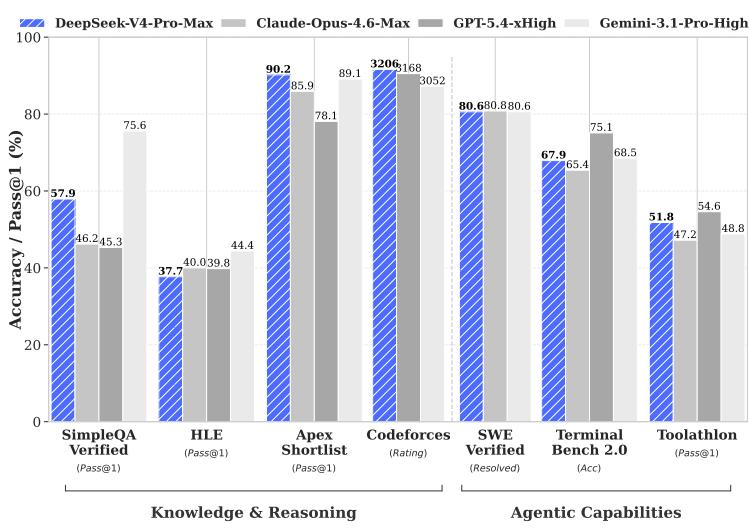
\includegraphics[keepaspectratio,alt={image}]{images/9ec06f82ba5dfc971283ebd43ceab8ad077c79dca8612398cb54c1daad3a6c69.jpg}}

\pandocbounded{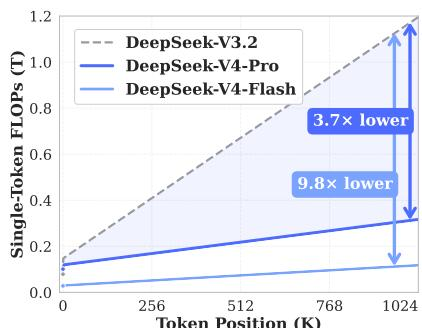
\includegraphics[keepaspectratio,alt={image}]{images/81b4091e91553eeaa965616c3c476f3a8ae0f1178b488cbade31a9dfb172be0a.jpg}}

\pandocbounded{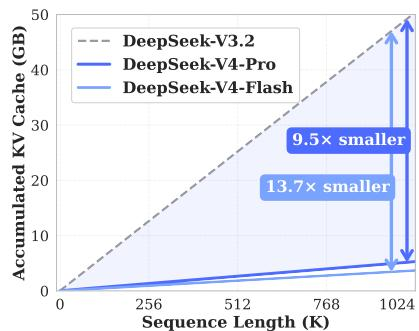
\includegraphics[keepaspectratio,alt={image}]{images/5c45e48fab463d34caba4b8f3b31d2222efefa82337895e12a0d75e9c2321833.jpg}}

Figure 1 \textbar{} Left: benchmark performance of DeepSeek-V4-Pro-Max
and its counterparts. Right:inference FLOPs and KV cache size of
DeepSeek-V4 series and DeepSeek-V3.2.

\section{Contents}\label{contents}

\section{1 Introduction 4}\label{introduction-4}

\section{2 Architecture 6}\label{architecture-6}

2.1 Designs Inherited from DeepSeek-V3 . 7

2.2 Manifold-Constrained Hyper-Connections 7

2.3 Hybrid Attention with CSA and HCA 9

2.3.1 Compressed Sparse Attention . . 9

2.3.2 Heavily Compressed Attention . 11

2.3.3 Other Details 12

2.3.4 Efficiency Discussion . 13

\section{2.4 Muon Optimizer 14}\label{muon-optimizer-14}

\section{3 General Infrastructures 15}\label{general-infrastructures-15}

3.1 Fine-Grained Communication-Computation Overlap in Expert Parallelism
. . . . 15

3.2 Flexible and Efficient Kernel Development with TileLang . . 16

3.3 High-Performance Batch-Invariant and Deterministic Kernel Libraries
. . . 18

3.4 FP4 Quantization-Aware Training . . . 19

3.5 Training Framework 20

3.5.1 Efficient Implementation of Muon 20

3.5.2 Cost-Effective and Memory-Efficient Implementation of mHC 21

3.5.3 Contextual Parallelism for Long-Context Attention 21

3.5.4 Extended Automatic Differentiation for Flexible Activation
Checkpointing 21

3.6 Inference Framework . 22

3.6.1 KV Cache Structure and Management . . 22

3.6.2 On-Disk KV Cache Storage . . 23

\section{4 Pre-Training 24}\label{pre-training-24}

4.1 Data Construction . 24

4.2 Pre-Training Setups . . . 25

4.2.1 Model Setups 25

4.2.2 Training Setups . . 25

4.2.3 Mitigating Training Instability 26

4.3 Evaluations 27

4.3.1 Evaluation Benchmarks 27

4.3.2 Evaluation Results 28

\section{5 Post-Training 29}\label{post-training-29}

5.1 Post-Training Pipeline 29

5.1.1 Specialist Training 29

5.1.2 On-Policy Distillation 32

5.2 RL and OPD Infrastructures 34

5.2.1 FP4 Quantization Integration . 34

5.2.2 Efficient Teacher Scheduling for Full-Vocabulary OPD 34

5.2.3 Preemptible and Fault-Tolerant Rollout Service 34

5.2.4 Scaling RL Framework for Million-Token Context . . 35

5.2.5 Sandbox Infrastructure for Agentic AI . . 35

5.3 Standard Benchmark Evaluation 36

5.3.1 Evaluation Setup . . 36

5.3.2 Evaluation Results 38

5.4 Performance on Real-World Tasks 41

5.4.1 Chinese Writing . . . 41

5.4.2 Search 42

5.4.3 White-Collar Task . 42

5.4.4 Code Agent . 44

\section{6 Conclusion, Limitations, and Future Directions
44}\label{conclusion-limitations-and-future-directions-44}

\section{A Author List and Acknowledgment
54}\label{a-author-list-and-acknowledgment-54}

A.1 Author List . 54

A.2 Acknowledgment . . 55

\section{B Evaluation Details 5 5}\label{b-evaluation-details-5-5}

\section{1. Introduction}\label{introduction}

The emergence of reasoning models (DeepSeek-AI, 2025; OpenAI, 2024c) has
established anew paradigm of test-time scaling, driving substantial
performance gains for Large LanguageModels (LLMs). However, this scaling
paradigm is fundamentally constrained by the quadraticcomputational
complexity of the vanilla attention mechanism (Vaswani et al., 2017),
whichcreates a prohibitive bottleneck for ultra-long contexts and
reasoning processes. Concurrently,the emergence of long-horizon
scenarios and tasks --- from complex agentic workflows tomassive
cross-document analysis --- has also made efficient support for
ultra-long contextscritical for future progress. While recent
open-source efforts (Bai et al., 2025a; DeepSeek-AI,2024; MiniMax, 2025;
Qwen, 2025) have advanced general capabilities, this core
architecturalinefficiency in handling ultra-long sequences remains a key
impediment, limiting further gainsfrom test-time scaling and hindering
further exploration into long-horizon scenarios and tasks.

In order to break the efficiency barrier in ultra-long contexts, we
develop the DeepSeek-V4series, including the preview versions of
DeepSeek-V4-Pro with 1.6T parameters (49B activated)and
DeepSeek-V4-Flash with 284B parameters (13B activated). Through
architectural innova-tions, DeepSeek-V4 series achieve a dramatic leap
in computational efficiency for processingultra-long sequences. This
breakthrough enables efficient support for a context length of
onemillion tokens, ushering in a new era of million-length contexts for
next-generation LLMs. Webelieve our capability to efficiently handle
ultra-long sequences unlocks the next frontier oftest-time scaling,
paves the way for deeper research into long-horizon tasks, and
establishes anecessary foundation for exploring future paradigms like
online learning.

Compared with the DeepSeek-V3 architecture (DeepSeek-AI, 2024),
DeepSeek-V4 seriesretain the DeepSeekMoE framework (Dai et al., 2024)
and Multi-Token Prediction (MTP) strategy,while introducing several key
innovations in architecture and optimization. To enhance long-context
efficiency, we design a hybrid attention mechanism combining Compressed
SparseAttention (CSA) and Heavily Compressed Attention (HCA). CSA
compresses the KV cachesalong the sequence dimension and then performs
DeepSeek Sparse Attention (DSA) (DeepSeek-AI, 2025), whereas HCA applies
more aggressive compression to the KV caches but keepsdense attention.
To strengthen modeling capability, we incorporate
Manifold-ConstrainedHyper-Connections (mHC) (Xie et al., 2026) that
upgrade conventional residual connections.Additionally, we introduce the
Muon (Jordan et al., 2024; Liu et al., 2025) optimizer to thetraining of
DeepSeek-V4 series, leading to faster convergence and improved training
stability.

To enable efficient training and inference for DeepSeek-V4 series as
well as productive de-velopment, we introduce several infrastructure
optimizations. First, we design and implementa single fused kernel for
MoE modules that fully overlaps computation, communication, andmemory
access. Second, we employ TileLang (Wang et al., 2026), a
Domain-Specific Language(DSL) to balance development productivity and
runtime efficiency. Third, we provide efficientbatch-invariant and
deterministic kernel libraries to ensure bitwise reproducibility across
train-ing and inference. Fourth, we incorporate FP4 quantization-aware
training for MoE expertweights and the indexer QK path to reduce memory
and computation. Fifth, for the trainingframework, we extend the
autograd framework with tensor-level checkpointing for
fine-grainedrecomputation control; and we enhance training efficiency
with a hybrid ZeRO strategy for theMuon optimizer, cost-effective mHC
implementations via recomputation and fused kernels, andtwo-stage
contextual parallelism to manage compressed attention. Finally, for the
inferenceframework, we design a heterogeneous KV cache structure with
on-disk storage strategies toenable efficient shared-prefix reuse.

By employing hybrid CSA and HCA, along with precision optimizations on
computationand storage, DeepSeek-V4 series achieve significantly lower
inference FLOPs and a substantiallyreduced KV cache size compared with
DeepSeek-V3.2, especially in long-context settings. Theright part of
Figure 1 demonstrates the estimated single-token inference FLOPs and
accumulatedKV cache size of DeepSeek-V3.2 and DeepSeek-V4 series. In the
scenario of 1M-token context,even DeepSeek-V4-Pro, which has a larger
number of activated parameters, attains only \(2 7 \%\)of the
single-token FLOPs (measured in equivalent FP8 FLOPs) and \(1 0 \%\) of
the KV cachesize relative to DeepSeek-V3.2. Furthermore,
DeepSeek-V4-Flash, with its smaller number ofactivated parameters,
pushes efficiency even further: in the 1M-token context setting, it
achievesonly \(1 0 \%\) of the single-token FLOPs and \(7 \%\) of the KV
cache size compared with DeepSeek-V3.2.Additionally, for DeepSeek-V4
series, the routed expert parameters utilize FP4 precision. Whilethe
peak FLOPs for \(\mathrm { F P 4 } \times \mathrm { F P 8 }\) operations
are currently the same as \(\mathrm { F P 8 } \times \mathrm { F P 8 }\)
on existinghardware, they can theoretically be implemented to be 1/3
more efficient on future hardware,which will further enhance the
efficiency of DeepSeek-V4 series.

During pre-training, we train DeepSeek-V4-Flash on 32T tokens and
DeepSeek-V4-Pro on 33Ttokens, respectively. After pre-training, these
two models can natively and efficiently support1M-length contexts. In
our internal evaluations, DeepSeek-V4-Flash-Base already
surpassesDeepSeek-V3.2-Base across a majority of benchmarks with its
more parameter-efficient design.DeepSeek-V4-Pro-Base further extends
this advantage to set a new performance standard amongDeepSeek
foundation models, achieving comprehensive superiority across reasoning,
coding,long-context, and world knowledge tasks.

The post-training pipeline of DeepSeek-V4 series features a two-stage
paradigm: the inde-pendent cultivation of domain-specific experts,
followed by unified model consolidation viaon-policy distillation (Lu
and Lab, 2025). Initially, for each target domain --- such as
mathematics,coding, agent, and instruction following --- a separate
expert model is trained independently.The base model first undergoes
Supervised Fine-Tuning (SFT) on high-quality, domain-specificdata to
establish foundational capabilities. Subsequently, Reinforcement
Learning (RL) is ap-plied using Group Relative Policy Optimization
(GRPO) (DeepSeek-AI, 2025), which furtheroptimizes the model for
domain-aligned behaviors guided by reward models tailored to
specificsuccess criteria. This phase yields a diverse set of specialized
experts, each excelling in itsrespective field. Finally, to integrate
these distinct proficiencies, a single unified model is trainedthrough
on-policy distillation, wherein the unified model acts as the student
learning to optimizethe reverse KL loss with teacher models.

\section{Summary of Core Evaluation
Results}\label{summary-of-core-evaluation-results}

• Knowledge: In assessments of broad world knowledge,
DeepSeek-V4-Pro-Max, the maxi-mum reasoning effort mode of
DeepSeek-V4-Pro, significantly outperforms leading open-source models on
the SimpleQA (OpenAI, 2024d) and Chinese-SimpleQA (He et al.,
2024)benchmarks. Regarding educational knowledge --- evaluated via
MMLU-Pro (Wang et al.,2024b), HLE (Phan et al., 2025), and GPQA (Rein et
al., 2023) --- DeepSeek-V4-Pro-Maxshows a marginal lead over its
open-source counterparts. DeepSeek-V4-Pro-Max hassignificantly closed
the gap with the leading proprietary model, Gemini-3.1-Pro, despitestill
trailing it in these knowledge-based evaluations.

• Reasoning: Through the expansion of reasoning tokens,
DeepSeek-V4-Pro-Max demon-strates superior performance relative to
GPT-5.2 and Gemini-3.0-Pro on standard reasoningbenchmarks.
Nevertheless, its performance falls marginally short of GPT-5.4 and
Gemini-3.1-Pro, suggesting a developmental trajectory that trails
state-of-the-art frontier models byapproximately 3 to 6 months.
Furthermore, DeepSeek-V4-Flash-Max achieves comparable

\pandocbounded{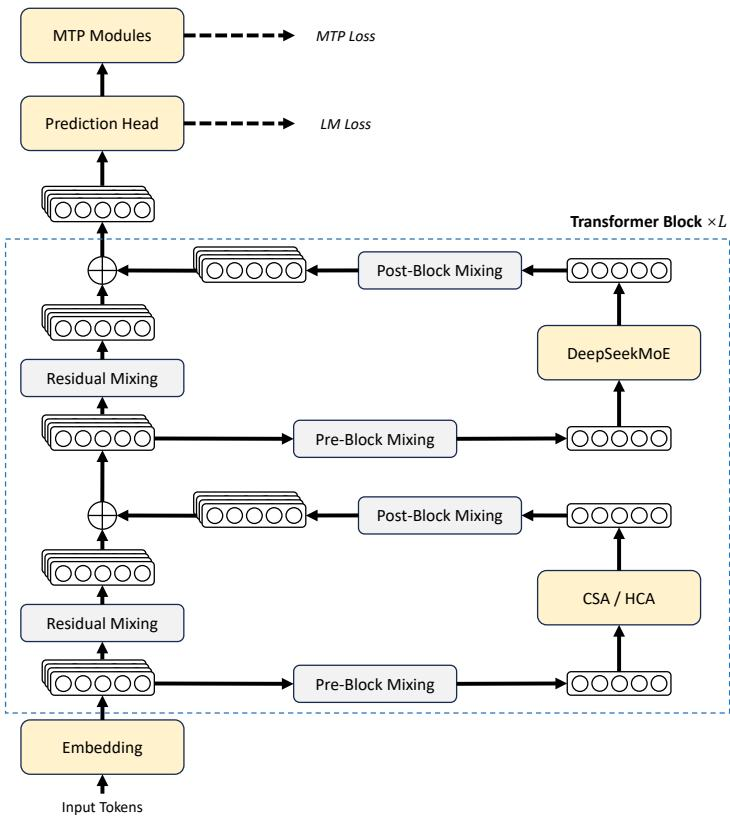
\includegraphics[keepaspectratio,alt={image}]{images/2c5ffc992a56d87715c81c76ccc8e01e6186c02cf3a03d4a75ca416f22237b79.jpg}}

Figure 2 \textbar{} Overall architecture of DeepSeek-V4 series. We use
hybrid CSA (Compressed SparseAttention) and HCA (Heavily Compressed
Attention) for attention layers, DeepSeekMoE forfeed-forward layers, and
strengthen conventional residual connections with mHC.

performance to GPT-5.2 and Gemini-3.0-Pro, establishing itself as a
highly cost-effectivearchitecture for complex reasoning tasks.

• Agent: On public benchmarks, DeepSeek-V4-Pro-Max is on par with
leading open-sourcemodels, such as Kimi-K2.6 and GLM-5.1, but slightly
worse than frontier closed models.In our internal evaluation,
DeepSeek-V4-Pro-Max outperforms Claude Sonnet 4.5 andapproaches the
level of Opus 4.5.

• Long-Context: DeepSeek-V4-Pro-Max delivers strong results on synthetic
and real usecases with a 1-million-token context window, surpassing even
Gemini-3.1-Pro on academicbenchmarks.

• DeepSeek-V4-Pro v.s. DeepSeek-V4-Flash: DeepSeek-V4-Flash-Max exhibits
lower per-formance in knowledge evaluations due to its smaller parameter
scale. However, itachieves comparable results on reasoning tasks when
allocated a larger thinking bud-get. In agent evaluations, while
DeepSeek-V4-Flash-Max matches the performance ofDeepSeek-V4-Pro-Max on
several benchmarks, it still trails its larger counterpart on
morecomplex, high-difficulty tasks.

\section{2. Architecture}\label{architecture}

Overall, DeepSeek-V4 series retain the Transformer (Vaswani et al.,
2017) architecture and Multi-Token Prediction (MTP) modules
(DeepSeek-AI, 2024; Gloeckle et al., 2024), while introducingseveral key
upgrades over DeepSeek-V3: (1) firstly, we introduce the
Manifold-ConstrainedHyper-Connections (mHC) (Xie et al., 2026) to
strengthen conventional residual connections;

\begin{enumerate}
\def\labelenumi{(\arabic{enumi})}
\setcounter{enumi}{1}
\tightlist
\item
  secondly, we design a hybrid attention architecture, which greatly
  improves long-contextefficiency through Compressed Sparse Attention
  and Heavily Compressed Attention. (3) thirdly,we employ Muon (Jordan
  et al., 2024; Liu et al., 2025) as the optimizer. For the
  Mixture-of-Experts (MoE) components, we still adopt the DeepSeekMoE
  (Dai et al., 2024) architecture, withonly minor adjustments from
  DeepSeek-V3. The Multi-Token Prediction (MTP) (DeepSeek-AI,2024;
  Gloeckle et al., 2024; Li et al., 2024; Qi et al., 2020) configuration
  remains identical tothat of DeepSeek-V3. All other unspecified details
  follow the settings established in DeepSeek-V3 (DeepSeek-AI, 2024).
  Figure 2 illustrates the overall architecture of DeepSeek-V4, and
  thedetails are described below.
\end{enumerate}

\section{2.1. Designs Inherited from
DeepSeek-V3}\label{designs-inherited-from-deepseek-v3}

Mixture-of-Experts. As previous DeepSeek-series models (DeepSeek-AI,
2024; DeepSeek-AI,2024), DeepSeek-V4 series also adopt the DeepSeekMoE
paradigm (Dai et al., 2024) for Feed-Forward Networks (FFNs), which sets
fine-grained routed experts and shared experts. Differentfrom
DeepSeek-V3, we change the activation function that computes the
affinity scores fromSigmoid(·) into Sqrt(Softplus(·)). For load
balancing, we also employ the auxiliary-loss-freestrategy (DeepSeek-AI,
2024; Wang et al., 2024a), augmented by a slight sequence-wise
balanceloss that prevents extreme imbalance within individual sequences.
For DeepSeek-V4, we removethe constraint on the number of routing target
nodes, and carefully redesign the parallelismstrategy to maintain
training efficiency. Furthermore, compared with DeepSeek-V3, we
replacethe dense FFN layers in the initial several Transformer blocks
with MoE layers that employHash routing (Roller et al., 2021). The Hash
routing strategy determines the target experts ofeach token according to
a predefined hash function with regard to the input token ID.

Multi-Token Prediction. As DeepSeek-V3, DeepSeek-V4 series also set MTP
modules andobjectives. Given that the MTP strategy has been validated in
DeepSeek-V3, we adopt the samestrategy for DeepSeek-V4 series without
modification.

\section{2.2. Manifold-Constrained
Hyper-Connections}\label{manifold-constrained-hyper-connections}

As shown in Figure 2, DeepSeek-V4 series incorporate
Manifold-Constrained Hyper-Connections(mHC) (Xie et al., 2026) to
strengthen the conventional residual connections between
adjacentTransformer blocks. Compared with naive Hyper-Connections (HC)
(Zhu et al., 2025), the coreidea of mHC is to constrain the residual
mapping onto a specific manifold, and thus enhance thestability of
signal propagation across layers while preserving model expressivity.
This subsectionbriefly introduces the standard HC and describes how we
design mHC for stable training.

Standard Hyper-Connections. The standard HC expands the width of the
residual streamby a factor of \(n _ { \mathrm { h c } }\) .
Specifically, the shape of the residual stream is expanded from
\(\mathbb { R } ^ { d }\) to
\(\mathbb { R } ^ { n _ { \mathrm { h c } } \times d }\) ,where \(d\) is
the hidden size of the actual layer input. Let
\(X _ { l } = [ \mathbf { x } _ { l , 1 } ; \ldots ; \mathbf { x } _ { l , n _ { \mathrm { h c } } } ] ^ { T } \in \mathbb { R } ^ { n _ { \mathrm { h c } } \times d }\)
be theresidual state before the ??-th layer. HC introduces three linear
mappings: an input
mapping\(A _ { l } \in \mathbb { R } ^ { 1 \times n _ { \mathrm { h c } } }\)
, a residual transformation
\(B _ { l } \in \mathbb { R } ^ { n _ { \mathrm { h c } } \times n _ { \mathrm { h c } } }\)
, and an output mapping
\(\bar { C _ { l } } \bar { \in } \mathbb { R } ^ { n _ { \mathrm { h c } } \times \bar { 1 } }\)
. Theupdate of the residual state is then formulated as:

\[
X _ {l + 1} = B _ {l} X _ {l} + C _ {l} \mathcal {F} _ {l} \left(A _ {l} X _ {l}\right), \tag {1}
\]

where \(\mathcal { F } _ { l }\) denotes the ??-th layer (e.g., an MoE
layer), whose input and output shapes are both\(\mathbb { R } ^ { d }\)
. Note that the actual layer input
\(A _ { l } X _ { l } \in \mathbb { R } ^ { d }\) is also \(d\)
-dimensional, so the expanded residual

width does not influence the design of the inner layers. HC decouples
the residual width fromthe actual hidden size, offering a complementary
scaling axis with minimal computationaloverhead, as
\(n _ { \mathrm { h c } }\) is typically much smaller than the hidden
size ??. However, even though HChas demonstrated potential in improving
model performance, we find that the training willfrequently exhibit
numerical instability when stacking multiple layers, which hinders the
scalingof HC.

Manifold-Constrained Residual Mapping. The core innovation of mHC is to
constrain theresidual mapping matrix \(B _ { l }\) to the manifold of
doubly stochastic matrices (the Birkhoff polytope)\(M _ { ☉ }\) , and
thus enhance the stability of signal propagation across layers:

\[
B _ {l} \in \mathcal {M} := \{M \in \mathbb {R} ^ {n \times n} \mid M \mathbf {1} _ {n} = \mathbf {1} _ {n}, \mathbf {1} _ {n} ^ {T} M = \mathbf {1} _ {n} ^ {T}, M \geqslant 0 \}. \tag {2}
\]

This constraint ensures that the spectral norm of the mapping matrix
\(\| B _ { l } \| _ { 2 }\) is bounded by 1, sothe residual
transformation is non-expansive, which increases the numerical stability
during boththe forward pass and backpropagation. Besides, the set M is
closed under multiplication, whichguarantees stability in the scenarios
of deep stacks of mHC. In addition, the input
transformation\(A _ { l }\) and output transformation \(C _ { l }\) are
also constrained to be non-negative and bounded via aSigmoid function to
avoid the risk of signal cancellation.

Dynamic Parameterization. The parameters of three linear mappings are
dynamically gen-erated, which are decomposed into a dynamic
(input-dependent) component and a static(input-independent) component.
Given the input
\(\bar { X _ { l } } \in \mathbb { R } ^ { n _ { \mathrm { h c } } \times d } .\)
, it is first flattened and normal-ized:
\(\hat { X } _ { l } = \bar { \mathrm { R M S N o r m } } ( \mathrm { v e c } ( X _ { l } ) ) \in \mathbb { R } ^ { 1 \times n _ { \mathrm { h c } } d }\)
. Then, we follow the conventional HC to generate theunconstrained raw
parameters
\(\tilde { A } _ { l } \in \mathbb { R } ^ { 1 \times n _ { \mathrm { h c } } }\)
,
\(\tilde { B } _ { l } \in \mathbb { R } ^ { n _ { \mathrm { h c } } \times n _ { \mathrm { h c } } }\)
, and
\(\tilde { C } _ { l } \in \mathbb { R } ^ { n _ { \mathrm { h c } } \times 1 }\)
:

\[
\tilde {A} _ {l} = \alpha_ {l} ^ {\text {p r e}} \cdot \left(\hat {X} _ {l} W _ {l} ^ {\text {p r e}}\right) + S _ {l} ^ {\text {p r e}}, \tag {3}
\]

\[
\tilde {B} _ {l} = \alpha_ {l} ^ {\mathrm {r e s}} \cdot \operatorname {M a t} \left(\hat {X} _ {l} W _ {l} ^ {\mathrm {r e s}}\right) + S _ {l} ^ {\mathrm {r e s}}, \tag {4}
\]

\[
\tilde {C} _ {l} = \alpha_ {l} ^ {\text {p o s t}} \cdot \left(\hat {X} _ {l} W _ {l} ^ {\text {p o s t}}\right) ^ {T} + S _ {l} ^ {\text {p o s t}}, \tag {5}
\]

where
\(W _ { l } ^ { \mathrm { p r e } } , W _ { l } ^ { \mathrm { p o s t } } \in \mathbb { R } ^ { n _ { \mathrm { h c } } d \times n _ { \mathrm { h c } } }\)
and
\(W _ { l } ^ { \mathrm { r e s } } \in \mathbb { R } ^ { n _ { \mathrm { h c } } d \times n _ { \mathrm { h c } } ^ { 2 } }\)
are learnable parameters for generating thedynamic components;
\(\mathrm { { M a t } ( \cdot ) }\) reshapes a vector of size
\(1 \times n _ { \mathrm { h c } } ^ { 2 }\) into a matrix of size
\(n _ { \mathrm { h c } } \times n _ { \mathrm { h c } } ;\)\(S _ { l } ^ { \mathrm { p r e } } \in \mathbb { R } ^ { 1 \times n _ { \mathrm { h c } } } , S _ { l } ^ { \mathrm { p o s t } } \in \mathbb { R } ^ { n _ { \mathrm { h c } } \times 1 } ,\)
, and
\(S _ { l } ^ { \mathrm { r e s } } \in \mathbb { R } ^ { n _ { \mathrm { h c } } \times n _ { \mathrm { h c } } }\)
are learnable static biases; and
\(\alpha _ { l } ^ { \mathrm { p r e } } , \alpha _ { l } ^ { \mathrm { r e s } } , \alpha _ { l } ^ { \mathrm { p o s t } } \in \mathbb { R }\)are
learnable gating factors initialized to small values.

Applying Parameter Constraints. After obtaining the unconstrained raw
parameters
\(\tilde { A } _ { l } , \tilde { B } _ { l } , \tilde { C } _ { l } ,\)we
then apply constraints described earlier to them to enhance the
numerical stability. To bespecific, for the input and output mappings,
we employ a Sigmoid function \(\sigma ( \cdot )\) to ensure
theirnon-negativity and boundedness:

\[
A _ {l} = \sigma (\tilde {A} _ {l}), \tag {6}
\]

\[
C _ {l} = 2 \sigma (\tilde {C} _ {l}). \tag {7}
\]

As for the residual mapping \({ \tilde { B } } _ { l } ,\) we project it
onto the manifold of doubly stochastic matrices \(\mathcal { M }\) .This
is achieved by the Sinkhorn-Knopp algorithm, which first applies an
exponential functionto \(\tilde { B } _ { l }\) to ensure positivity,
getting \(M ^ { ( 0 ) } = \exp ( \tilde { B } _ { l } ) ,\) , and then
iteratively performs column and rownormalization:

\[
M ^ {(t)} = \mathcal {T} _ {r} \left(\mathcal {T} _ {c} \left(M ^ {(t - 1)}\right)\right), \tag {8}
\]

where \(\mathcal { T } _ { r }\) and \(\mathcal { T } _ { c }\) denote
row and column normalization, respectively. This iteration converges toa
constrained doubly stochastic matrix
\(B _ { l } = M ^ { ( t _ { \operatorname* { m a x } } ) }\) . We choose
\(t _ { \mathrm { m a x } } = 2 0\) as a practical value.

\pandocbounded{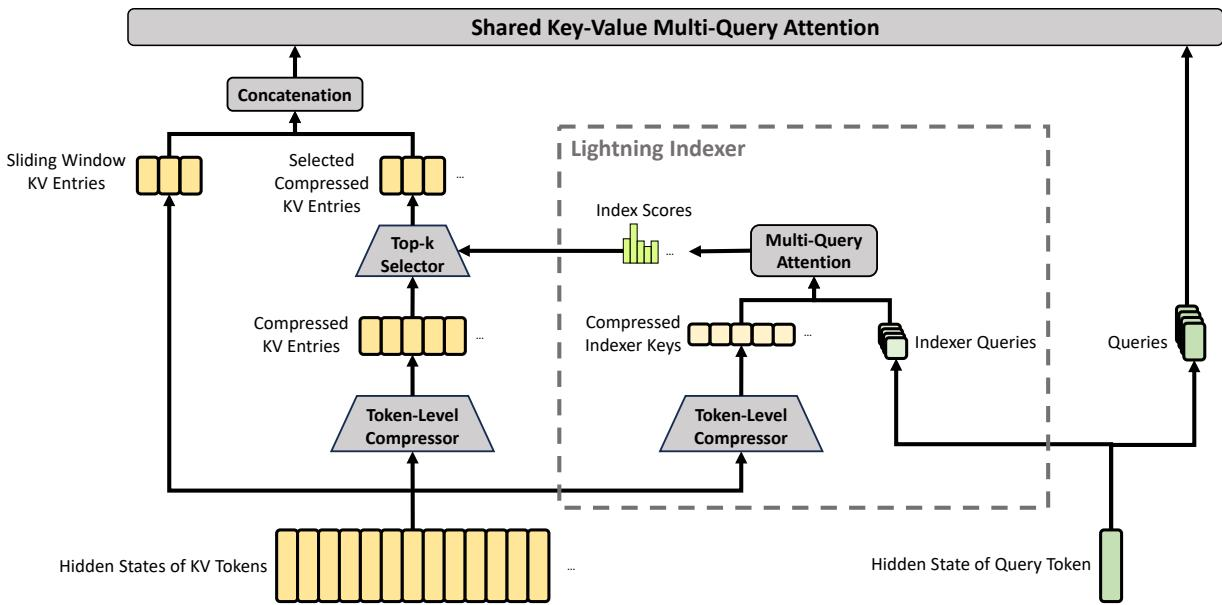
\includegraphics[keepaspectratio,alt={image}]{images/cff2b362b699adbc334a2f504449cbfbb7010bb6f736884475dc536b11b1d80b.jpg}}

Figure 3 \textbar{} Core architectures of CSA. It compresses the number
of KV entries to \(\textstyle { \frac { 1 } { m } }\) times, andthen
applies DeepSeek Sparse Attention for further acceleration.
Additionally, a small set ofsliding window KV entries is combined with
the selected compressed KV entries to enhancelocal fine-grained
dependencies.

\section{2.3. Hybrid Attention with CSA and
HCA}\label{hybrid-attention-with-csa-and-hca}

As the context length reaches extreme scales, the attention mechanism
emerges as the dominantcomputational bottleneck in a model. For
DeepSeek-V4, we design two efficient attentionarchitectures ---
Compressed Sparse Attention (CSA) and Heavily Compressed Attention
(HCA)--- and employ their interleaved hybrid configuration, which
substantially reduces the compu-tational cost of attention in long-text
scenarios. CSA integrates both compression and sparseattention
strategies: it first compresses the Key-Value (KV) cache of every ??
tokens into oneentry, and then applies DeepSeek Sparse Attention (DSA)
(DeepSeek-AI, 2025) where each querytoken attends to only \(k\)
compressed KV entries. HCA aims for extreme compression by
consol-idating the KV cache of every
\(m ^ { \prime } \left( \gg m \right)\) tokens into a single entry. The
hybrid architecture ofCSA and HCA remarkably improves the long-context
efficiency of DeepSeek-V4 series, makingone-million-token context
feasible in practice. This subsection describes the core techniquesof
our hybrid attention architecture, and we also provide an open-source
implementation1 tospecify more details unambiguously.

\section{2.3.1. Compressed Sparse
Attention}\label{compressed-sparse-attention}

The core architecture of CSA is illustrated in Figure 3, which first
compresses the KV cache of each\(m\) tokens into one entry, and then
applies DeepSeek Sparse Attention for further acceleration.

Compressed Key-Value Entries. Let
\(H \in \mathbb { R } ^ { n \times d }\) be a sequence of input hidden
states, where\(n\) is the sequence length and \(d\) is the hidden size.
CSA first computes two series of KV
entries\(C ^ { a } , C ^ { b } \in \mathbb { R } ^ { \bar { n } \times c }\)
and their corresponding compression weights
\(Z ^ { a } , { \bar { Z } } ^ { b } \in \mathbb { R } ^ { n \times c }\)
, where \(c\) is the head

dimension:

\[
C ^ {a} = H \cdot W ^ {a K V}, \quad C ^ {b} = H \cdot W ^ {b K V}, \tag {9}
\]

\[
Z ^ {a} = H \cdot W ^ {a Z}, \quad Z ^ {b} = H \cdot W ^ {b Z}, \tag {10}
\]

where
\(W ^ { a K V } , W ^ { b K V } , W ^ { a Z } , W ^ { b Z } \in \mathbb { R } ^ { d \times c }\)
are trainable parameters. Next, each ?? KV entries in \(C ^ { a }\)
and\(C ^ { b }\) will be compressed into one entry according to their
compression weights and learnablepositional biases \(B ^ { a }\)
\(\mathbf { \Phi } ^ { a } , B ^ { b } \in \mathbb { R } ^ { m \times c }\)
, producing
\(C ^ { \mathsf { C o m p } } \in \mathbb { R } ^ { \frac { n } { m } \times c }\)
. Each compressed entry
\(C _ { i } ^ { \mathrm { C o m p } } \in \mathbb { R } ^ { c }\)
iscomputed by

\[
\left[ S _ {m i: m (i + 1) - 1} ^ {a}; S _ {m (i - 1): m i - 1} ^ {b} \right] = \operatorname {S o f t m a x} _ {\text {r o w}} \left(\left[ Z _ {m i: m (i + 1) - 1} ^ {a} + B ^ {a}; Z _ {m (i - 1): m i - 1} ^ {b} + B ^ {b} \right]\right), \tag {11}
\]

\[
C _ {i} ^ {\text {C o m p}} = \sum_ {j = m i} ^ {m (i + 1) - 1} S _ {j} ^ {a} \odot C _ {j} ^ {a} + \sum_ {j = m (i - 1)} ^ {m i - 1} S _ {j} ^ {b} \odot C _ {j} ^ {b}, \tag {12}
\]

where \(\odot\) denotes the Hadamard product; Softmaxrow(·) denotes the
softmax operation alongthe row dimension, which performs normalization
across the total of \(2 m\) elements from both\(Z ^ { a }\) and
\(Z ^ { b }\) . When \(i = 0\) ,
\(Z _ { m ( i - 1 ) : m i - 1 } ^ { b }\) is padded with negative
infinity and \(C _ { m ( i - 1 ) : m i - 1 } ^ { b }\) is paddedwith
zeros. Note that each \(C _ { i } ^ { \mathrm { C o m p } }\) is derived
from 2?? KV entries, but the indexes of \(C ^ { b }\) used
for\(C _ { i } ^ { \mathrm { C o m p } }\) and the indexes of
\(C ^ { a }\) used for ????−1
\(C _ { i - 1 } ^ { \mathsf { C o m p } }\) are overlapped. Therefore,
CSA in fact compressesthe sequence length to \(\frac { 1 } { m }\)
times.

Lightning Indexer for Sparse Selection. After obtaining the compressed
KV entries \(C ^ { \mathrm { C o m p } }\)CSA applies the DSA strategy
to select top-k compressed KV entries for core attention. First,CSA
performs the same compression operation used for
\(C ^ { \mathrm { C o m p } }\) to get compressed indexer
keys\(K ^ { \mathrm { I C o m i p } } \in \mathbb { R } ^ { \frac { n } { m } \times c ^ { I } } .\)
, where \(c ^ { I }\) is the indexer head dimension. Then, for a query
token \(t ,\) we producethe indexer queries
\(\{ \mathbf { q } _ { t , 1 } ^ { I } ; \mathbf { q } _ { t , 2 } ^ { I } ; . . . ; \mathbf { q } _ { t , n _ { h } ^ { I } } ^ { I } \}\)
in a low-rank manner:

\[
\mathbf {c} _ {t} ^ {Q} = \mathbf {h} _ {t} \cdot W ^ {D Q}, \tag {13}
\]

\[
[ \mathbf {q} _ {t, 1} ^ {I}; \mathbf {q} _ {t, 2} ^ {I}; \dots ; \mathbf {q} _ {t, n _ {h} ^ {I}} ^ {I} ] = \mathbf {q} _ {t} ^ {I} = \mathbf {c} _ {t} ^ {Q} \cdot W ^ {I U Q}, \tag {14}
\]

where \(\mathbf { h } _ { t } \ \in \ \mathbb { R } ^ { d }\) is the
input hidden state of the query token ??;
\(\mathbf { c } _ { t } ^ { Q } \in \mathbb { R } ^ { d _ { c } }\) is
the compressedlatent vector for queries; \(d _ { c }\) denotes the query
compression dimension; \(n _ { h } ^ { I }\) denotes the numberof
indexer query heads;
\(W ^ { D Q } \in \mathbb { R } ^ { d \times d _ { c } }\) and
\(W ^ { I U Q } \in \mathbb { R } ^ { d _ { c } \times c ^ { I } n _ { h } ^ { I } }\)
are the down-projection and up-projection matrices for indexer queries,
respectively. Next, the index score \(I _ { t , s } \in \mathbb { R }\)
between thequery token ?? and a preceding compressed block ??
\(\textstyle { \bigl ( } s < \operatorname { F l o o r } ( { \frac { t } { m } } ) { \bigr ) }\)
is computed by

\[
\left[ w _ {t, 1} ^ {I}; w _ {t, 2} ^ {I}; \dots ; w _ {t, n _ {h} ^ {I}} ^ {I} \right] = \mathbf {w} _ {t} ^ {I} = \mathbf {h} _ {t} \cdot W ^ {w}, \tag {15}
\]

\[
I _ {t, s} = \sum_ {h = 1} ^ {n _ {h} ^ {I}} w _ {t, h} ^ {I} \cdot \operatorname {R e L U} \left(\mathbf {q} _ {t, h} ^ {I} \cdot K _ {s} ^ {\text {I C o m p}}\right), \tag {16}
\]

where \(W ^ { w } \in \mathbb { R } ^ { d \times n _ { h } ^ { I } }\)
is a learnable matrix;
\(\boldsymbol { w _ { t , h } ^ { I } } \in \mathbb { R }\) is the
weight of the \(h\) -th indexer head. For aquery token \(t ,\) given its
index scores \(I _ { t , : \prime }\) we employ a top-
\(\mathbf { \nabla } \cdot \mathbf { k }\) selector to selectively
retain a subsetof compressed KV entries
\(C _ { t } ^ { \mathsf { S p r s C o m p } }\) for subsequent core
attention:

\[
C _ {t} ^ {\text {S p r s C o m p}} = \left\{C _ {s} ^ {\text {C o m p}} \mid I _ {t, s} \in \operatorname {T o p - k} \left(I _ {t,:}\right) \right\}. \tag {17}
\]

\pandocbounded{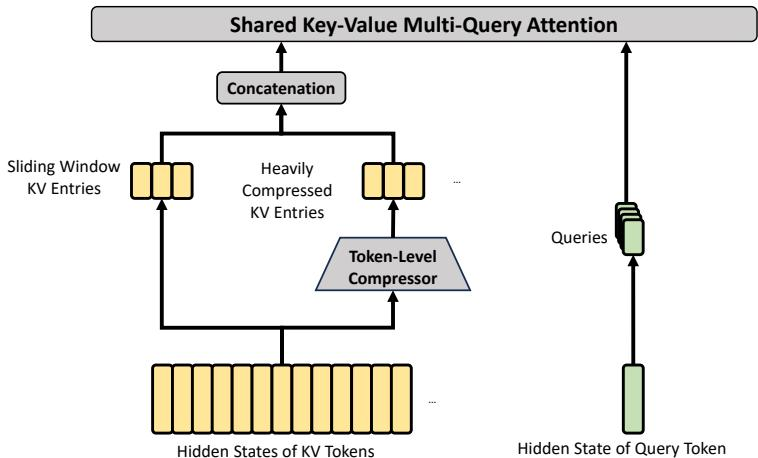
\includegraphics[keepaspectratio,alt={image}]{images/3be80607df218b3fca89c7c8159b93be4102ea887a2d41db75764756d19c0dc0.jpg}}

Figure 4 \textbar{} Core architectures of HCA. It performs heavier
compression, where the KV entries
of\(m ^ { \prime } \left( \gg m \right)\) tokens will be consolidated
into one. Also, we additionally introduce a small set ofsliding window
KV entries to enhance local fine-grained dependencies.

Shared Key-Value MQA. After selecting the sparse KV entries, CSA then
performs coreattention in a Multi-Query Attention (MQA) (Shazeer, 2019)
manner, where each compressedKV entry in
\(C _ { t } ^ { \mathsf { S p r s C o m p } }\) serves as both attention
key and value. To be specific, for a query token \(t ,\)we first produce
attention queries
\(\{ \mathbf { q } _ { t , 1 } ; \mathbf { q } _ { t , 2 } ; . . . ; \mathbf { q } _ { t , n _ { h } } \}\)
from the compressed latent vector \(\mathbf { c } _ { t } ^ { Q }\) :

\[
\left[ \mathbf {q} _ {t, 1}; \mathbf {q} _ {t, 2}; \dots ; \mathbf {q} _ {t, n _ {h}} \right] = \mathbf {q} _ {t} = \mathbf {c} _ {t} ^ {Q} \cdot W ^ {U Q}, \tag {18}
\]

where \(n _ { h }\) denotes the number of query heads;
\(W ^ { U Q } \in \mathbb { R } ^ { d _ { c } \times c n _ { h } }\) is
the up-projection matrices forqueries. Note that the latent query vector
\(\mathbf { c } _ { t } ^ { Q }\) is shared with that used for the
indexer queries.Next, we perform MQA on \{q??,??\} and CSprsComp?? :
\(\{ \pmb q _ { t , i } \}\)
\(C _ { t } ^ { \mathsf { S p r s C o m p } }\)

\[
\mathbf {o} _ {t, i} = \text {C o r e A t t n} \left(\text {q u e r y} = \mathbf {q} _ {t, i}, \text {k e y} = C _ {t} ^ {\text {S p r s C o m p}}, \text {v a l u e} = C _ {t} ^ {\text {S p r s C o m p}}\right), \tag {19}
\]

where \(\mathbf { o } _ { t , i } \in \mathbb { R } ^ { c }\) is the
core attention output of the ??-th head at the ??-th token; CoreAttn(·)
denotesthe core attention operation.

Grouped Output Projection. In the configuration of DeepSeek-V4,
\(c n _ { h }\) is quite large. Therefore,directly projecting the
outputs of the core attention operation
\(\left[ \mathbf { o } _ { t , 1 } ; \mathbf { o } _ { t , 2 } ; . . . ; \mathbf { o } _ { t , n _ { h } } \right] = \mathbf { o } _ { t } \in \mathbb { R } ^ { c n _ { h } }\)
to a\(d\) -dimensional hidden state will impose a substantial
computational burden. To mitigate thiscost, we design a grouped output
projection strategy. To be specific, we first split \(n _ { h }\)
outputsinto ?? groups, and then for each group of output
\({ \mathbf o } _ { t , i } ^ { G } \in \mathbb { R } ^ { c \frac { n _ { h } } { g } }\)
, we project it to a \(d _ { g }\) -dimensionalintermediate output
\({ \mathbf o } _ { t , i } ^ { G ^ { \prime } } \in \mathbb { R } ^ { d _ { g } }\)
, where \(d _ { g } \ < \ c \frac { n _ { h } } { g }\) . Finally, we
project the intermediate
output\([ \mathbf { o } _ { t , 1 } ^ { G ^ { \prime } } ; \mathbf { o } _ { t , 2 } ^ { G ^ { \prime } } ; . . . ; \mathbf { o } _ { t , g } ^ { G ^ { \prime } } ] \in \mathbb { R } ^ { d _ { g } g }\)
to the final attention output
\(\hat { \mathbf { o } } _ { t } \in \mathbb { R } ^ { d }\) .

\section{2.3.2. Heavily Compressed
Attention}\label{heavily-compressed-attention}

The core architecture of HCA is illustrated in Figure 4, which
compresses the KV cache in aheavier manner, but does not employ sparse
attention.

Compressed Key-Value Entries. By and large, the compression strategy of
HCA is similar tothat of CSA, but employs a larger compression rate
\(m ^ { \prime }\) \(( \gg m )\) ) and does not perform overlapped

compression. Let \(H \in \mathbb { R } ^ { n \times d }\) be a sequence
of input hidden states, HCA first computes theoriginal KV entries
\(C \in \mathbb { R } ^ { n \times c }\) and their corresponding
compression weights \(Z \in \mathbb { R } ^ { n \times c }\) :

\[
C = H \cdot W ^ {K V}, \tag {20}
\]

\[
Z = H \cdot W ^ {Z}, \tag {21}
\]

where \(W ^ { K V }\) , \(W ^ { Z } \in \mathbb { R } ^ { d \times c }\)
are trainable parameters. Next, each ??′ KV entries in \(C\) will be
compressedinto one according to the compression weights and learnable
positional biases
\(B \in \mathbb { R } ^ { m ^ { \prime } \times c }\)producing
\(C ^ { \mathsf { C o m p } } \in \mathbb { R } ^ { \frac { n } { m ^ { \prime } } \times c }\)
. Each compressed entry
\(C _ { i } ^ { \mathrm { C o m p } } \in \mathbb { R } ^ { c }\) is
computed by

\[
S _ {m ^ {\prime} i: m ^ {\prime} (i + 1) - 1} = \operatorname {S o f t m a x} _ {\text {r o w}} \left(Z _ {m ^ {\prime} i: m ^ {\prime} (i + 1) - 1} + B\right), \tag {22}
\]

\[
C _ {i} ^ {\text {C o m p}} = \sum_ {j = m ^ {\prime} i} ^ {m ^ {\prime} (i + 1) - 1} S _ {j} \odot C _ {j}. \tag {23}
\]

Through this compression operation, HCA compresses the sequence length
to \(\scriptstyle { \frac { 1 } { m ^ { \prime } } }\) times.

Shared Key-Value MQA and Grouped Output Projection. HCA also employs the
shared KVMQA and grouped output projection strategies as CSA does. After
the KV compression, for aquery token ??, HCA first produces attention
queries
\(\{ \mathbf { q } _ { t , 1 } ; \mathbf { q } _ { t , 2 } ; . . . ; \mathbf { q } _ { t , n _ { h } } \}\)
in a low-rank manner:

\[
\mathbf {c} _ {t} ^ {Q} = \mathbf {h} _ {t} \cdot W ^ {D Q}, \tag {24}
\]

\[
[ \mathbf {q} _ {t, 1}; \mathbf {q} _ {t, 2}; \dots ; \mathbf {q} _ {t, n _ {h}} ] = \mathbf {q} _ {t} = \mathbf {c} _ {t} ^ {Q} \cdot W ^ {U Q}, \tag {25}
\]

where \(\mathbf h _ { t } \in \mathbb R ^ { d }\) is the input hidden
state of the query token \(t ; n _ { h }\) denotes the number of
queryheads; \(W ^ { D Q } \in \mathbb { R } ^ { d \times d _ { c } }\)
and \(W ^ { U Q } \in \mathbb { R } ^ { d _ { c } \times c n _ { h } }\)
are the down-projection and up-projection matrices forqueries,
respectively. Next, we perform MQA on
\(\{ \mathbf { q } _ { t , i } \}\) and \(C ^ { \mathrm { C o m p } }\)
:

\[
\mathbf {o} _ {t, i} = \text {C o r e A t t n} \left(\text {q u e r y} = \mathbf {q} _ {t, i}, \text {k e y} = C ^ {\text {C o m p}}, \text {v a l u e} = C ^ {\text {C o m p}}\right), \tag {26}
\]

where \(\mathbf { o } _ { t , i } \in \mathbb { R } ^ { c }\) is the
core attention output of the ??-th head at the \(t\) -th token. Next, as
CSA does,HCA splits \(n _ { h }\) outputs into ?? groups, and for each
group of output
\({ \mathbf o } _ { t , i } ^ { G } \in \mathbb { R } ^ { c \frac { n _ { h } } { g } }\)
, HCA projects itto a \(d _ { g }\) -dimensional intermediate output
\({ \mathbf o } _ { t , i } ^ { G ^ { \prime } } \in \mathbb { R } ^ { d _ { g } }\)
, where \(d _ { g } < c \frac { n _ { h } } { g }\) . Finally, HCA
projects theintermediate output
\([ \mathbf { o } _ { t , 1 } ^ { G ^ { \prime } } ; \mathbf { o } _ { t , 2 } ^ { G ^ { \prime } } ; . . . ; \mathbf { o } _ { t , g } ^ { G ^ { \prime } } ] \in \mathbb { R } ^ { d _ { g } g }\)
to the final attention output \$ \{ \hat { \mathbf { o } } \} \_ \{ t \}
\in \mathbb { R } \^{} \{ d \}\$ .

\section{2.3.3. Other Details}\label{other-details}

In addition to the core architectures of CSA and HCA described above,
our hybrid attentionincorporates several other techniques. For writing
clarity, we omit these additional techniquesfrom the above introduction
and will briefly describe them in this subsection. Also, this
subsec-tion focuses only on the core ideas of them and may omit some
tiny details for simplicity. Weencourage the readers to refer to our
open-source implementation for unambiguous details.

Query and Key-Value Entry Normalization. For both CSA and HCA, we
perform an addi-tional RMSNorm operation on each head of the queries and
the only head of the compressed KVentries, just before the core
attention operation. This normalization avoids exploding attentionlogits
and may improve training stability.

Partial Rotary Positional Embedding. For both CSA and HCA, we partially
employ the RotaryPositional Embedding (RoPE) (Su et al., 2024) to the
attention queries, KV entries, and the coreattention outputs. To be
specific, for each query vector and KV entry vector used in CSA andHCA,
we apply RoPE to its last 64 dimensions. Since the KV entries serve as
both attentionkeys and values, the naive core attention outputs
\(\left\{ \mathbf { o } _ { t , i } \right\}\) will carry absolute
position embeddings,derived from the weighted sum of KV entries. As a
countermeasure, we also apply RoPE withposition \(- i\) on the last 64
dimensions of each \(\mathbf { o } _ { t , i }\) . In this way, the
output of the core attentionwill also carry relative position embeddings
--- the contribution of each KV entry to the coreattention outputs will
also be related to the distance between the query and the KV entry.

Additional Branch of Sliding Window Attention. In order to strictly
preserve causality inCSA and HCA, each query attends to only preceding
compressed KV blocks. Consequently, aquery cannot access information
from other tokens within its own compressed block. Meanwhile,recent
tokens usually possess greater relevance to the query token in language
modeling. Forthese reasons, we introduce a supplementary attention
branch to both CSA and HCA in a slidingwindow manner, for better
modeling of local dependencies. To be specific, for each query token,we
additionally produce \(n _ { \mathrm { w i n } }\) uncompressed KV
entries corresponding to the recent \(n _ { \mathrm { w i n } }\)
tokens.In the core attention of CSA and HCA, these KV entries in the
sliding window will be usedalong with the compressed KV entries.

Attention Sink. In the core attention of CSA and HCA, we employ the
trick of attentionsink (OpenAI, 2025; Xiao et al., 2024). To be
specific, we set a series of learnable sink
logits\(\{ z _ { 1 } ^ { \prime } , z _ { 2 } ^ { \prime } , . . . , z _ { n _ { h } } ^ { \prime } \}\)
. For the \(h \cdot\) -th attention head,
\(\mathrm { E x p } ( z _ { h } ^ { \prime } )\) will be added to the
denominator of theattention score:

\[
s _ {h, i, j} = \frac {\operatorname {E x p} \left(z _ {h , i , j}\right)}{\sum_ {k} \operatorname {E x p} \left(z _ {h , i , k}\right) + \operatorname {E x p} \left(z _ {h} ^ {\prime}\right)}, \tag {27}
\]

where \(s _ { h , i , j } , z _ { h , i , j } \in \mathbb { R }\) denote
the attention score and attention logit of the \(h\) -th attention
headbetween the ??-th query token and the \(j \cdot\) -th preceding
token or compressed block. This techniqueallows each query head to
adjust its total attention scores to be not equal to 1, and even to
benear 0.

\section{2.3.4. Efficiency Discussion}\label{efficiency-discussion}

Due to the employment of hybrid CSA and HCA, together with low-precision
computationand storage, the attention module of DeepSeek-V4 series
achieves remarkable efficiency in bothattention FLOPs and KV cache size,
especially in long-context scenarios. First, we adopt amixed storage
format for KV entries: BF16 precision is used for the rotary positional
embedding(RoPE) dimensions, while FP8 precision is applied to the
remaining dimensions. This hybridrepresentation reduces the KV cache
size by nearly half compared with pure BF16 storage.Second, attention
computation within the lightning indexer is performed in FP4
precision,which accelerates the attention operation under extremely long
contexts. Third, relative toDeepSeek-V3.2, a smaller attention top-k is
chosen in DeepSeek-V4 series, thereby improvingmodel efficiency on
short- and medium-length texts. Finally, and most importantly,
compressedattention and hybrid attention techniques substantially reduce
both the KV cache size and thecomputational FLOPs.

Taking BF16 GQA8 (Ainslie et al., 2023) with a head dimension of 128 as
the baseline --- oneof the common configurations of LLM attention ---
the KV cache size of DeepSeek-V4 series canbe dramatically reduced to
approximately \(2 \%\) times of that baseline in the 1M-context setting.

Algorithm 1 Muon Optimizer for DeepSeek-V4

Require: Learning rate \(\eta\) , momentum \(\mu\) , weight decay
\(\lambda\) , update rescaling factor \(\gamma\)\\
1: for each training step \(t\) do\\
2: for each logically independent weight
\(W \in \mathbb{R}^{n \times m}\) do\\
3: \(G_{t} = \nabla_{W} \mathcal{L}_{t}(W_{t-1})\)\\
4: \(M_{t} = \mu M_{t-1} + G_{t}\)\\
5: \(O_{t}' = \text{Hybrid NewtonSchulz}(\mu M_{t} + G_{t})\)\\
6: \(O_{t} = O_{t}' \cdot \sqrt{\max(n, m)} \cdot \gamma\)\\
7: \(W_{t} = W_{t-1} \cdot (1 - \eta \lambda) - \eta O_{t}\)\\
8: end for\\
9: end for

Moreover, even when compared with DeepSeek-V3.2 (DeepSeek-AI, 2025) ---
already an efficientbaseline --- DeepSeek-V4 series still exhibits
substantial advantages in efficiency. A comparisonof their inference
FLOPs and KV cache size is provided in the right part of Figure 1.

\section{2.4. Muon Optimizer}\label{muon-optimizer}

We employ the Muon (Jordan et al., 2024; Liu et al., 2025) optimizer for
the majority of modulesin DeepSeek-V4 series due to its faster
convergence and improved training stability. The fullalgorithm of our
Muon optimization is summarized in Algorithm 1.

Basic Configurations. We maintain the AdamW (Loshchilov and Hutter,
2017) optimizer forthe embedding module, the prediction head module, the
static biases and gating factors ofmHC modules, and the weights of all
RMSNorm modules. All other modules are updated withMuon. Following Liu
et al.~(2025), we also apply weight decay to Muon parameters, use
theNesterov (Jordan et al., 2024; Nesterov, 1983) trick, and rescale the
Root Mean Square (RMS) ofthe update matrix for reutilization of our
AdamW hyper-parameters. Different from them, weuse hybrid Newton-Schulz
iterations for orthogonalization.

Hybrid Newton-Schulz Iterations. For a given matrix ??, let its Singular
Value Decomposition(SVD) be \(M = U \Sigma V ^ { T }\) . The
Newton-Schulz iterations aim to approximately orthogonalize ?? to
be\(U V ^ { T }\) . Usually, \(M\) will be first normalized as
\(M _ { 0 } = M / | | \boldsymbol { M } | | _ { F }\) to ensure its
maximum singular valuedoes not exceed 1. Then, each Newton-Schulz
iteration performs the following operation:

\[
M _ {k} = a M _ {k - 1} + b \left(M _ {k - 1} M _ {k - 1} ^ {T}\right) M _ {k - 1} + c \left(M _ {k - 1} M _ {k - 1} ^ {T}\right) ^ {2} M _ {k - 1}. \tag {28}
\]

Our hybrid Newton-Schulz performs 10 iterations over two distinct
stages. During the first 8steps, we use coefficients
\(( a , b , c ) = ( 3 . 4 4 4 5 , - 4 . 7 7 5 0 , 2 . 0 3 1 5 )\) to
drive rapid convergence, bringingthe singular values close to 1. In the
final 2 steps, we switch to coefficients
\(( a , b , c ) = ( 2 , - 1 . 5 , 0 . 5 ) _ { . }\) ,which stabilize the
singular values precisely at 1.

Avoiding Exploding Attention Logits. The attention architecture of
DeepSeek-V4 series al-lows us to directly apply RMSNorm on the attention
queries and KV entries, which effectivelyprevents attention logits from
exploding. Consequently, we do not employ the QK-Clip tech-nique (Liu et
al., 2025) in our Muon optimizer.

\section{3. General Infrastructures}\label{general-infrastructures}

\section{3.1. Fine-Grained Communication-Computation Overlap in Expert
Parallelism}\label{fine-grained-communication-computation-overlap-in-expert-parallelism}

Mixture-of-Experts (MoE) can be accelerated via Expert Parallelism (EP).
However, EP re-quires complex inter-node communication and imposes
substantial demands on interconnectbandwidth and latency. To alleviate
the communication bottleneck in EP and achieve higherend-to-end
performance under lower interconnection bandwidth requirements, we
proposea fine-grained EP scheme that fuses communication and computation
into a single pipelinedkernel for communication-computation overlapping.

Communication Latency Can Be Hidden. The key insight of our EP scheme is
that thecommunication latency can be effectively hidden beneath
computation in MoE layers. As shownin Figure 5, in DeepSeek-V4 series,
each MoE layer can be decomposed mainly into four stages:two
communication-bound stages, Dispatch and Combine, and two
computation-bound stages,Linear-1 and Linear-2. Our profiling reveals
that within a single MoE layer, the total time ofcommunication is less
than that of the computation. Therefore, after fusing communication
andcomputation into a unified pipeline, computation remains the dominant
bottleneck, implyingthat the system can tolerate lower interconnect
bandwidth without degrading end-to-endperformance.

\begin{enumerate}
\def\labelenumi{(\alph{enumi})}
\tightlist
\item
  Naive Solution
\end{enumerate}

\pandocbounded{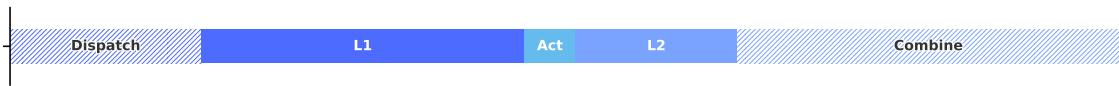
\includegraphics[keepaspectratio,alt={image}]{images/f2ac4523895a5705584644bf4da73ddd23ac322af58e6d2291935e790c9fe5bc.jpg}}

\begin{enumerate}
\def\labelenumi{(\alph{enumi})}
\setcounter{enumi}{1}
\tightlist
\item
  Comet
\end{enumerate}

\pandocbounded{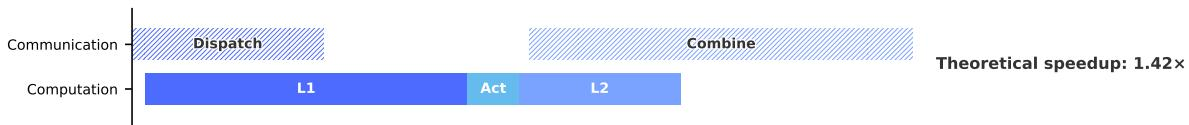
\includegraphics[keepaspectratio,alt={image}]{images/f525fd1a5cb552ce5b9a894259033d70ef4d8f2447ace4bc72cd0c1a8062d7ae.jpg}}

\begin{enumerate}
\def\labelenumi{(\alph{enumi})}
\setcounter{enumi}{2}
\tightlist
\item
  Ours
\end{enumerate}

\pandocbounded{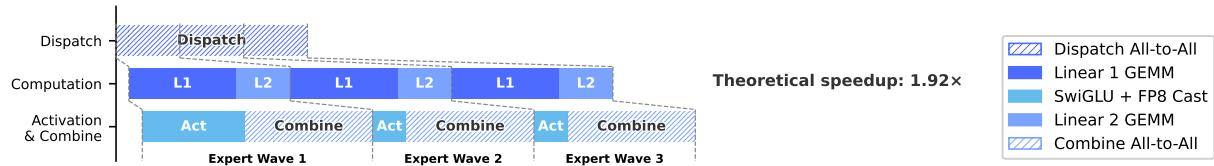
\includegraphics[keepaspectratio,alt={image}]{images/b626abcfe97688178c9180f4a61338b18821e9443ba872ab14ed8278c6d8f829.jpg}}

Figure 5 \textbar{} Illustration of our EP scheme with related works.
Comet (Zhang et al., 2025b) overlapsDispatch with Linear-1, and Linear-2
with Combine, separately. Our EP scheme achieves a finer-grained
overlapping by splitting and scheduling experts into waves. The
theoretical speedup isevaluated in the configuration of the
DeepSeek-V4-Flash architecture.

Fine-Grained EP Scheme. To further lower the interconnect bandwidth
requirement andamplify the benefits of overlapping, we introduce a
finer-grained expert partitioning scheme.Inspired by many related works
(Aimuyo et al., 2025; Zhang et al., 2025b), we split and schedulethe
experts into waves. Each wave consists of a small portion of experts. As
soon as all expertswithin the wave have completed their communication,
computation can commence immediatelywithout waiting for other experts.
In steady state, computation of current wave, token transfer forthe next
wave, and result sending of completed experts all proceed concurrently,
as demonstratedin Figure 5. This forms a fine-grained pipeline among
experts, keeping both computation andcommunication continuous throughout
the wave. The wave-based scheduling speeds up the

performance on extreme cases such as Reinforcement Learning (RL)
rollout, which usuallyencounters long-tail small batches.

Performance and Open-Sourced Mega-Kernel. We validated the fine-grained
EP schemeon both NVIDIA GPUs and HUAWEI Ascend NPUs platforms. Compared
against strongnon-fused baselines, it achieves
\(1 . 5 0 \sim 1 . 7 3 \times\) speedup for general inference workloads,
andup to \(1 . 9 6 \times\) for latency-sensitive scenarios such as RL
rollouts and high-speed agent serving.We have open-sourced the
CUDA-based mega-kernel implementation named MegaMoE2 as acomponent of
DeepGEMM.

Observations and Proposals. We share observations and lessons from
kernel developmentand offer some proposals to hardware vendors, in the
hope of aiding efficient hardware designand achieving better
software-hardware co-design:

• Computation-Communication Ratio. Full communication-computation
overlap hingeson the computation-communication ratio, rather than the
bandwidth solely. Denoting peakcompute throughput as ?? and interconnect
bandwidth as ??, communication can be fullyhidden when
\(C / B \leqslant V _ { \mathrm { c o m p } } / V _ { \mathrm { c o m m } } ,\)
where \(V _ { \mathrm { c o m p } }\) denotes the computation volume and
\(V _ { \mathrm { { c o m m } } }\)refers to the communication volume.
For DeepSeek-V4-Pro, where each token-expertpair requires 6ℎ?? FLOPs
(SwiGLU gate, up, and down projections) but only \(3 h\) bytes
ofcommunication (FP8 Dispatch \(^ +\) BF16 Combine), this simplifies to:

\[
\frac {C}{B} \leqslant 2 d = 6 1 4 4 \mathrm {F L O P s / B y t e}.
\]

That is, each GBps of interconnect bandwidth suffices to hide the
communication for 6.1TFLOP/s of compute. Once bandwidth meets this
threshold, it ceases to be the bottleneck,and devoting additional
silicon area to further bandwidth brings diminishing returns.We
encourage future hardware designs to target such balance points rather
than scalebandwidth unconditionally.

• Power Budget. Extreme kernel fusion drives compute, memory, and
network to highload simultaneously, making power throttling a key
performance limiter. We suggest thatfuture hardware designs provide
sufficient power headroom for such fully concurrentworkloads.

• Communication Primitives. We adopt a pull-based approach where each
GPU activelyreads data from remote GPUs, avoiding the high notification
latency that fine-grainedpush entails. Future hardware with
lower-latency cross-GPU signaling would make pushviable and enable more
natural communication patterns.

• Activation Function. We propose replacing SwiGLU with a low-cost
element-wise activa-tion that involves no exponential or division
operations. This lightens the post-GEMMprocessing directly, and under
the same parameter budget, removing the gate projectionenlarges the
intermediate dimension \(d\) , further relaxing the bandwidth
requirement.

\section{3.2. Flexible and Efficient Kernel Development with
TileLang}\label{flexible-and-efficient-kernel-development-with-tilelang}

In practice, our elaborate model architecture would have resulted in
hundreds of fine-grainedTorch ATen operators. We adopt TileLang (Wang et
al., 2026) to develop a set of fused kernelsto replace the vast majority
of them, delivering optimal performance with minimal effort. It

also allows us to quickly prototype operators like attention variants
during validation. Thesekernels play critical roles in model
architecture development, large-scale training, and ultimatelyproduction
deployment of inference services. As a Domain-Specific Language (DSL),
TileLangbalances development productivity with runtime efficiency,
enabling rapid development whilesupporting deep, iterative optimizations
within the same codebase. Additionally, we collab-orate closely with the
TileLang community to foster a more agile, efficient, and stable
kerneldevelopment workflow.

Reducing Invocation Overhead with Host Codegen. As accelerators continue
to grow inperformance, CPU-side orchestration overhead becomes
increasingly prominent. For small,highly optimized kernels, such fixed
host overhead can easily cap utilization and throughput.A common source
of this overhead is that host-side logic, such as runtime contract
checks, istypically written in Python for flexibility and thus incurs a
fixed per-invocation cost.

We mitigate this overhead with Host Codegen, which moves most host-side
logic into gen-erated host code. Specifically, we first co-generate the
device kernel and a lightweight hostlauncher at the IR (Intermediate
Representation) level, embedding the necessary metadata---suchas data
types, rank/shape constraints, and stride/layout assumptions---parsed
from the lan-guage frontend. The launcher is then lowered to the host
source code built on top of theTVM-FFI (Chen et al., 2018) framework,
whose compact calling convention and zero-copy tensorinterop together
minimize host-side overhead. At runtime, this generated host code
performsvalidation and argument marshaling, shifting all per-invocation
checks out of the Python exe-cution path. Our measurements show that
CPU-side validation overhead drops from tens orhundreds of microseconds
to less than one microsecond per invocation.

SMT-Solver-Assisted Formal Integer Analysis. TileLang kernels involve
complex tensorindex arithmetic that requires strong formal integer
analysis. During compilation passes suchas layout inference, memory
hazard detection, and bound analysis, the compiler must verifywhether
integer expressions satisfy specific properties to enable the
corresponding optimiza-tions. Therefore, stronger formal analysis
capabilities can unlock more advanced and complexoptimization
opportunities.

To this end, we integrate the Z3 SMT solver (De Moura and Bjørner, 2008)
into TileLang'salgebraic system, providing formal analysis capability
for most integer expressions in tensorprograms. We strike a balance
between computational overhead and formal expressiveness bytranslating
TileLang's integer expressions into Z3's quantifier-free non-linear
integer arithmetic(QF\_NIA). Based on Integer Linear Programming (ILP)
solvers, QF\_NIA seamlessly resolvesstandard linear integer expressions
common in kernels. Furthermore, its inherent non-linearreasoning
capacity effectively addresses advanced challenges like vectorization
over variabletensor shapes. Under reasonable resource limits, Z3
elevates overall optimization performancewhile restricting compilation
time overhead to just a few seconds. The impact is substantialacross
multiple passes, including vectorization, barrier insertion, and code
simplification.

Numerical Precision and Bitwise Reproducibility. In production settings,
numerical correct-ness and reproducibility are as critical as raw
throughput. We therefore prioritize accuracy bydefault: fast-math
optimizations are disabled at the compiler level, and
precision-affecting ap-proximations are provided only as explicit,
opt-in frontend operators (e.g., T.\_\_exp, T.\_\_log,and T.\_\_sin).
Conversely, when strict IEEE-754 semantics are required, TileLang
provides

IEEE-compliant intrinsics with explicit rounding modes (e.g.,
T.ieee\_fsqrt, T.ieee\_fdiv,and T.ieee\_add), enabling developers to
precisely specify numerical behavior.

We also target bitwise reproducibility for validating kernels against
hand-written CUDAbaselines. We align TileLang's algebraic simplification
and lowering rules with mainstreamCUDA toolchains (e.g., NVCC) to avoid
transformations that introduce unintended bit-leveldifferences. Layout
annotations (e.g., T.annotate\_layout) further allow users to pin
downlayout-dependent lowering decisions, keeping evaluation and
accumulation order consistentwith the reference CUDA implementation and
thus enabling bit-identical outputs when desired.

Our evaluation shows that these accuracy- and reproducibility-oriented
design choices donot sacrifice performance: under conservative defaults,
TileLang kernels remain competitive,while exposing knobs to selectively
relax numerical constraints for higher speed.

\section{3.3. High-Performance Batch-Invariant and Deterministic Kernel
Libraries}\label{high-performance-batch-invariant-and-deterministic-kernel-libraries}

To enable efficient training and inference, we develop a comprehensive
set of high-performancecomputational kernels. Beyond basic
functionalities and maximizing hardware utilization,another pivotal
design goal is to ensure training reproducibility and bitwise alignment
amongpre-training, post-training, and inference pipelines. Therefore, we
implement end-to-end,bitwise batch-invariant, and deterministic kernels
with minimal performance overhead. Thesekernels are helpful for
debugging, stability analysis, and consistent post-training behavior.

Batch Invariance. Batch invariance ensures that the output of any given
token remains bitwiseidentical, regardless of its position within a
batch. To implement batch invariance, the primarychallenges are listed
as follows:

• Attention. To achieve batch invariance, we cannot use the split-KV
method (Dao et al.,2023), which distributes the attention computation
for a single sequence across multipleStream Multiprocessors (SMs) to
balance the load of SMs. However, abandoning thistechnique will lead to
severe wave-quantization problems3, which can adversely affectGPU
utilization. To address this, we develop a dual-kernel strategy for
batch-invariantdecoding. The first kernel computes the attention output
for an entire sequence withina single SM, ensuring high throughput for
fully occupied waves. The second kernel, tominimize the latency of the
final partially-filled wave and thus alleviate wave-quantization,uses
multiple SMs for a single sequence. For the bitwise identity of these
two kernels,we carefully design the calculation path of the second
kernel to ensure its accumulationorder is the same as that of the first
kernel. Additionally, the second kernel utilizes dis-tributed shared
memory4 within thread-block clusters, enabling high-speed data
exchangeacross SMs. This dual-kernel method effectively confines the
overhead of batch-invariantdecoding to be negligible.

• Matrix Multiplication. Traditional cuBLAS library (NVIDIA Corporation,
2024) cannotachieve batch invariance. Therefore, we replace it
end-to-end with DeepGEMM (Zhaoet al., 2025). Furthermore, for very small
batch sizes, conventional implementation usuallyemploys split-k (Osama
et al., 2023) techniques to improve performance. Unfortunately,split-k
techniques cannot guarantee batch invariance, a pivotal feature in
DeepSeek-V4.

Therefore, we abandon split-k in most scenarios, which, however, may
cause performancedegradation. To address this, we introduce a set of
optimizations that enable our imple-mentation of matrix multiplication
to match or even surpass the performance of standardsplit-k in most
major scenarios.

Determinism. Deterministic training is highly beneficial for debugging
hardware or softwareissues. Moreover, when training exhibits anomalies
such as loss spikes, determinism enablesresearchers to more easily
pinpoint numerical causes and further refine the model design.
Non-determinism in training typically stems from non-deterministic
accumulation order, often dueto the use of atomic addition instructions.
This issue primarily occurs during the backward pass,notably at the
following parts:

• Attention Backward. In conventional implementations of backward
propagation forsparse attention, we use atomicAdd to accumulate
gradients for the KV tokens. Thisintroduces non-determinism due to the
non-associativity of floating-point addition. Toaddress this problem, we
allocate separate accumulation buffers for each SM, followed bya global
deterministic summation across all buffers.

• MoE Backward. When multiple SMs from different ranks concurrently
write data tothe same buffer on a receiving rank, negotiating writing
positions also introduces non-determinism. To resolve this, we design a
token order pre-processing mechanism withineach single rank, combined
with buffer isolation across multiple ranks. This strategyensures
determinism of both the send results of expert parallelism and the
accumulationorder in the MoE backward pass.

• Matrix Multiplication in mHC. mHC involves a matrix multiplication
with an output di-mension of only 24. For very small batch sizes, we are
compelled to use the split-k (Osamaet al., 2023) algorithm, whose naive
implementation will cause non-determinism. Toovercome this, we output
each split part separately and perform a deterministic reductionin a
subsequent kernel, thereby preserving both performance and determinism.

\section{3.4. FP4 Quantization-Aware
Training}\label{fp4-quantization-aware-training}

To achieve inference acceleration and memory savings at deployment, we
introduce Quantization-Aware Training (QAT) (Jacob et al., 2018) during
the post-training stage, enabling the modelto adapt to the precision
degradation introduced by quantization. We apply FP4 (MXFP4)quantization
(Rouhani et al., 2023) to two components: (1) MoE expert weights, which
are amajor source of GPU memory occupancy (OpenAI, 2025), and (2) the
Query-Key (QK) pathin the indexer of CSA, where QK activations are
cached, loaded, and multiplied entirely inFP4, accelerating attention
score computation in long-context scenarios. In addition, we
furtherquantize the index scores \(I _ { : , i }\) : from FP32 to BF16
during this QAT process. This optimizationachieves a \(2 \times\)
speedup for the top-k selector, while preserving a \(9 9 . 7 \%\) recall
rate of KV entries.

For MoE expert weights, following the common practice of QAT, the FP32
master weightsmaintained by the optimizer are first quantized to FP4,
then dequantized back to FP8 forcomputation. Notably, our FP4-to-FP8
dequantization is lossless. This is because FP8 (E4M3)has 2 additional
exponent bits compared with FP4 (E2M1), offering a larger dynamic
range.Consequently, as long as the ratio between the maximum and minimum
scale factors of the FP4sub-blocks
\(\mathbf { \nabla } ^ { 1 \times 3 2 }\) tiles) within each FP8
quantization block \(1 2 8 \times 1 2 8\) tiles) does not exceeda
certain threshold, the fine-grained scale information can be fully
absorbed by the extendeddynamic range of FP8. We empirically verify that
current weights satisfy this condition. Thisallows the entire QAT
pipeline to fully reuse the existing FP8 training framework without

any modification. In the backward pass, gradients are computed with
respect to the same FP8weights in the forward pass and directly
propagated back to the FP32 master weights, equivalentto applying the
Straight-Through Estimator (STE) through the quantization operation.
This alsoavoids the need to re-quantize transposed weights.

During the inference and rollout phases of RL training, which do not
involve backwardpasses, we directly use real FP4 quantized weights
instead of simulated quantization. Thisensures that model behavior
during sampling is fully consistent with online deployment, whilealso
reducing kernel memory loading for actual speedup and significantly
lowering memoryconsumption. We process the QK path in the indexer of CSA
similarly.

\section{3.5. Training Framework}\label{training-framework}

Our training framework is built upon the scalable and efficient
infrastructure developed forDeepSeek-V3 (DeepSeek-AI, 2024). In training
DeepSeek-V4, we inherit this robust foundationwhile introducing several
key innovations to accommodate its novel architectural components
---specifically the Muon optimizer, mHC, and the hybrid attention
mechanism --- while maintaininghigh training efficiency and stability.

\section{3.5.1. Efficient Implementation of
Muon}\label{efficient-implementation-of-muon}

The Muon optimizer requires the full gradient matrix to compute
parameter updates, whichpresents a challenge when combined with the Zero
Redundancy Optimizer (ZeRO) (Rajbhandariet al., 2020). Traditional ZeRO
is designed for element-wise optimizers like AdamW, where asingle
parameter matrix can be partitioned and updated across multiple ranks.
To address thisconflict, we design a hybrid strategy of ZeRO bucket
assignment for Muon.

For dense parameters, we limit the maximum size of ZeRO parallelism and
employ aknapsack algorithm to assign parameter matrices to these ranks,
ensuring each rank manages aroughly balanced load. The bucket on each
rank is padded to match the size of the largest bucketacross ranks,
facilitating efficient reduce-scatter operations. This padding typically
incurs lessthan \(1 0 \%\) memory overhead in our setup, where each rank
manages no more than five parametermatrices. When the overall size of
data parallelism exceeds the limit for ZeRO, we computethe Muon update
redundantly across the extra data-parallel groups, trading computation
forreduced total bucket memory.

For MoE parameters, we optimize each expert independently. We first
flatten all downprojection matrices in SwiGLU (Shazeer, 2020) of all
experts across all layers, followed byflattened up projection matrices
and gate matrices. Then, we pad the flattened vector to ensurewe can
evenly distribute this vector across all ranks without splitting any
logically independentmatrix. Given the large number of experts, we do
not impose a limit of ZeRO parallelism forMoE parameters, and the
padding overhead is also negligible.

Additionally, on each rank, consecutive parameters of identical shape
will be automaticallymerged, enabling batched execution of the
Newton-Schulz iterations for better hardware utiliza-tion. Furthermore,
we observe that the Newton-Schulz iterations in Muon remain stable
whencomputed with BF16 matrix multiplications. Leveraging this, we
further quantize, in a stochasticrounding manner, the MoE gradients to
be synchronized across data-parallel ranks to the BF16precision, halving
the communication volume. To avoid accumulation errors introduced
bylow-precision adders, we replace conventional tree- or ring-based
reduce-scatter collectives witha two-phase approach. First, an
all-to-all operation exchanges local gradients across ranks, andthen
each rank performs a local sum in FP32. This design maintains numerical
robustness.

\section{3.5.2. Cost-Effective and Memory-Efficient Implementation of
mHC}\label{cost-effective-and-memory-efficient-implementation-of-mhc}

The introduction of mHC increases both activation memory consumption and
communicationvolume between pipeline stages, compared with conventional
residual connections. To mitigatethese costs, we implement several
optimization strategies.

Firstly, we carefully design and implement fused kernels of mHC for both
training andinference. Secondly, we introduce a recomputation strategy
that selectively checkpoints interme-diate tensors. Specifically, we
recompute most hidden states between layers and all normalizedlayer
inputs, while avoiding recomputation of compute-intensive operations.
This achieves abalance between memory saving and computational overhead.
Thirdly, we adjust the DualPipe1F1B overlapping scheme to accommodate
the increased pipeline communication and enableconcurrent execution of
some operations in mHC.

Collectively, these optimizations constrain the wall-time overhead of
mHC to only \(6 . 7 \%\) ofthe overlapped 1F1B pipeline stage. More
details of the engineering optimization can be foundin the dedicated mHC
paper (Xie et al., 2026).

\section{3.5.3. Contextual Parallelism for Long-Context
Attention}\label{contextual-parallelism-for-long-context-attention}

Conventional Context Parallelism (CP) partitions the sequence dimension,
with each rankmaintaining contiguous ?? tokens. This introduces two
challenges to our compressed attentionmechanisms (i.e., CSA and HCA). On
the one hand, training samples are packed from multiplesequences, and
each sequence is compressed independently by a factor of \(m\) (or
\(m ^ { \prime }\) ), with anytrailing tokens fewer than ?? being
discarded. Consequently, the compressed KV lengths aretypically less
than \(\frac { s } { m }\) and vary across ranks. On the other hand, the
compression requires ??consecutive KV entries, which may straddle the
boundary between two neighboring CP ranks.

To address these challenges, we design a two-stage communication
approach. In the firststage, each rank ?? sends its last ?? uncompressed
KV entries to rank \(i + 1\) . Then, rank \(i + 1\)compresses some of
these received entries together with its local ?? uncompressed KV
entries,producing a fixed length of
\(\textstyle { \frac { s } { m } } + 1\) compressed entries, in which
exist some padding entries. Inthe second stage, an all-gather operation
across all CP ranks collects the locally compressed KVentries. Then, a
fused select-and-pad operator reorganizes them into the full set of
compressedKV entries with a total length of cp\_size ·
\(\frac { s } { m }\) . Any padding entries are placed at the tail.
ForHCA and the indexer in CSA, the visible range of compressed KV
entries for each query tokencan be precomputed by rules. For the sparse
attention in CSA, the top- \(k\) selector explicitlyspecifies the
indices of visible compressed KV entries for each query.

\section{3.5.4. Extended Automatic Differentiation for Flexible
Activation
Checkpointing}\label{extended-automatic-differentiation-for-flexible-activation-checkpointing}

Conventional activation checkpointing implementations operate at the
granularity of an entiremodule, deciding whether to retain or recompute
its output activations during the backwardpass. This coarse granularity
often leads to suboptimal trade-offs between recomputation costand
activation memory footprint. An alternative approach is to manually
implement the forwardand backward logic of an entire layer, explicitly
managing tensor checkpointing states. Whileenabling fine-grained
control, this method loses the convenience of the automatic
differentiationframework, substantially increasing development
complexity.

To achieve fine-grained control without sacrificing programming
efficiency, we implement atensor-level activation checkpointing
mechanism with automatic differentiation support. Withthis mechanism,
developers only need to implement the forward pass and selectively
annotate

individual tensors for automatic checkpointing and recomputation. Our
framework leveragesTorchFX (Reed et al., 2022) to trace the full
computation graph. For each annotated tensor, itperforms a backward
traversal to identify the minimal subgraph required for its
recomputation.We define these minimal subgraphs as recomputation graphs
and insert them into the backwardlogic just before the corresponding
gradient computation.

Compared with the manual implementation, this design introduces no
additional overheadduring training. Recomputation in this framework is
implemented by directly freeing theGPU memory of the annotated tensor
and reusing the storage pointer from the recomputedtensor, without any
GPU memory copy. Furthermore, since graph tracing executes the
modelconcretely, we can track the underlying storage pointer of each
tensor, which enables automaticdeduplication of recomputation for
tensors that share storage (e.g., the input and output of areshape
operation). This relieves developers from reasoning about low-level
memory detailswhen annotating recomputation.

\section{3.6. Inference Framework}\label{inference-framework}

Our inference framework largely inherits from that of DeepSeek-V3, with
some differences inKV Cache management.

\section{3.6.1. KV Cache Structure and
Management}\label{kv-cache-structure-and-management}

To efficiently manage the heterogeneous KV caches arising from the
hybrid attention mechanismin DeepSeek-V4, we design a customized KV
cache layout. The layout is illustrated in Figure 6,and we will
elaborate on it in detail as follows.

Heterogeneous KV Entries in DeepSeek-V4. The hybrid attention mechanism
in DeepSeek-V4 series introduces multiple types of KV entries with
different Key-Value (KV) cache sizesand update rules. The lightning
indexer for sparse selection introduces additional dimensionsinto the KV
cache that possess embedding sizes distinct from those in the primary
attention.of 1 \(\frac { 1 } { m }\) comand
\(\begin{array} { r } { \frac { 1 } { m ^ { \prime } } . } \end{array}\)
ssion techniques employed in CSA and HCA reduce the sequence length by
factors, respectively, thereby decreasing the overall KV cache size. As
a result, KV cachesizes vary across different layers. Furthermore,
Sliding Window Attention (SWA) layers alsooperate with distinct KV cache
sizes, as well as separate cache hit and eviction policies. Inthe
compression branch, one KV entry is generated for every ?? tokens. When
the numberof remaining tokens is insufficient for compression, all
pending tokens and their associatedhidden states must be retained in a
buffer until the compression operation can be executed.These buffered
tokens represent a sequence state determined by positional context and
are alsomanaged within the KV cache framework.

Challenges in Managing Hybrid Attention KV Cache. The hybrid attention
mechanismviolates fundamental assumptions behind PagedAttention and its
variants. Although recenthybrid KV cache managing algorithms (e.g.,
Jenga (Zhang et al., 2025a), Hymba (Dong et al.,2025)) target general
hybrid attention models or specific structures, two principal
obstaclesprevent consolidating KV caches across all layers under the
PagedAttention framework:

• Diverse cache policies, such as those used in Sliding Window
Attention.

• Constraints imposed by high-performance attention kernels, including
alignment require-ments.

\pandocbounded{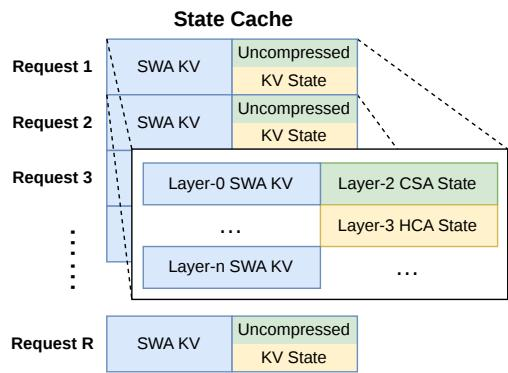
\includegraphics[keepaspectratio,alt={image}]{images/8ff12c133c03a2b14799e17f210141b34549caddea4948c4b7e8a173ffa24a15.jpg}}

\pandocbounded{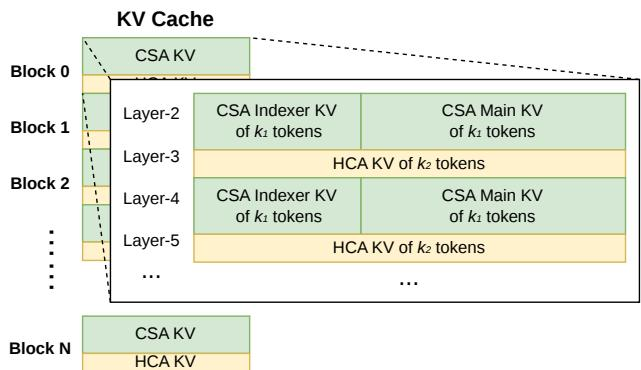
\includegraphics[keepaspectratio,alt={image}]{images/800a99ab9f9feb3ebdc99b4393370f0adc02c831d08080111240efd26617b7ba.jpg}}

Figure 6 \textbar{} Illustration of the KV cache Layout for DeepSeek-V4.
The KV cache is organized intotwo primary components: a classical KV
cache for CSA/HCA, and a state cache for SWA andunready-for-compression
tokens in CSA/HCA. In the state cache, each request is assigned
afixed-size cache block. Within this block, the SWA segment stores the
KV entries correspondingto the most recent \(n _ { \mathrm { w i n } }\)
tokens, while the CSA/HCA segment stores uncompressed tail statesthat
are not yet ready for compression. In the classical KV cache, we
allocate multiple blocksper request. Each cache block covers
\(\mathrm { l c m } ( m , m ^ { \prime } )\) original tokens, producing
\(\begin{array} { r } { k _ { 1 } = \frac { \operatorname { l c m } \tilde { ( } m , m ^ { \prime } ) } { m } } \end{array}\)
CSAcompressed tokens and ??2 = lcm(??,??′)??′
\(\begin{array} { r } { k _ { 2 } = \frac { \operatorname { l c m } ( m , m ^ { \prime } ) } { m ^ { \prime } } } \end{array}\)
m' HCA compressed tokens.

For efficient KV cache management of DeepSeek-V4, we design
corresponding strategies toovercome these two challenges.

State Cache for SWA and Uncompressed Tail Tokens. To address the first
obstacle, we adoptan alternative cache management mechanism. Since SWA
is designed to enhance performanceunder a limited KV cache size, it is
reasonable to treat it, along with the uncompressed tail tokensfrom the
compression branch, as a state-space model. The corresponding KV cache
can thus beregarded as a sequence-specific state that depends solely on
the current position. Accordingly,we pre-allocate a fixed- and
limited-size pool of state caches, and dynamically assign it to
eachsequence.

Sparse Attention Kernel Co-Design. Regarding the second obstacle,
conventional high-performance attention kernels typically assume a fixed
number ?? of tokens per block to optimizeperformance, corresponding to
\(B \cdot m\) original tokens in CSA and \(B \cdot m ^ { \prime }\) in
HCA. Through em-ploying a high-performance sparse-attention kernel,
different layers can accommodate variabletokens per block without
performance degradation. Achieving this requires co-designing theKV
cache layout and the sparse attention kernel. For instance, padding
blocks to align withcache lines can improve performance. Thus, for CSA
with compression ratio \(m\) and HCA withratio \(m ^ { \prime }\) , the
number of original tokens per block can be any multiple of
\(\operatorname { l c m } ( m , m ^ { \prime } )\) , the leastcommon
multiple of these two compression ratios.

\section{3.6.2. On-Disk KV Cache
Storage}\label{on-disk-kv-cache-storage}

When serving DeepSeek-V4, we leverage an on-disk KV cache storage
mechanism to eliminaterepeated prefilling for shared-prefix requests.
For the compressed KV entries in CSA/HCA andthe uncompressed KV entries
in Sliding Window Attention (SWA), we design separate solutionsfor
storage management.

For CSA and HCA, we simply store all of the compressed KV entries to the
disk. Whena request hits a stored prefix, we read and reuse the
compressed KV entries correspondingto the prefix, until the last
complete compression block. Specially, for prefix tokens in the
tailincomplete block, we still need to recompute them to restore the
uncompressed KV entries, asuncompressed KV entries in CSA and HCA are
not stored.

For the SWA KV entries, since they are not compressed and exist in every
layer, their volumeis approximately 8 times larger than the compressed
CSA and HCA KV entries. To handlethese large SWA KV entries efficiently,
we propose and implement three distinct strategies formanaging on-disk
SWA KV entries, each offering a different trade-off between storage
overheadand computational redundancy:

• Full SWA Caching. This strategy stores the complete SWA KV entries for
all tokens,ensuring computational zero-redundancy. Under this strategy,
the SWA KV entries of thehitting prefix can be reconstructed by just
reading the on-disk cache of the last \(n _ { \mathrm { w i n } }\)
tokenswithin that prefix. Despite computational zero-redundancy, this
strategy is inefficient formodern SSD-based storage systems --- only a
small subset of the stored SWA KV cachewill be accessed for each hitting
request, which leads to an unbalanced write-intensiveaccess pattern.

• Periodic Checkpointing. This strategy checkpoints SWA KV entries of
the last \(n _ { \mathrm { w i n } }\) tokenswithin every \(p\) tokens,
where \(p\) is a tunable parameter. For a hitting prefix, we load
themost recent checkpointed state, and then recompute the remaining tail
tokens. Throughtuning \(p ,\) , this strategy enables an on-demand
trade-off between storage and computation.

• Zero SWA Caching. This strategy does not store any SWA KV entries. For
a hitting prefix,we need to perform more recomputation to restore the
SWA KV entries. To be specific, ineach attention layer, the SWA KV entry
of each token depends on the SWA KV entries ofonly the most recent
\(n _ { \mathrm { W i n } }\) tokens from the previous layer. Therefore,
leveraging cachedCSA and HCA KV entries, recomputing the last
\(n _ { \mathrm { w i n } } \cdot L\) tokens is enough to restore the
last\(n _ { \mathrm { w i n } }\) SWA KV entries for an ??-layer model.

Depending on specific deployment scenarios, we select the most suitable
strategy to achieve thedesired trade-off between storage and
computation.

\section{4. Pre-Training}\label{pre-training}

\section{4.1. Data Construction}\label{data-construction}

On top of the pre-training data of DeepSeek-V3, we endeavor to construct
a more diverse andhigher-quality training corpus with longer effective
contexts. We continually refine our data con-struction pipelines. For
web-sourced data, we implement filtering strategies to remove
batchedauto-generated and templated content, thereby mitigating the risk
of model collapse (Zhu et al.,2024). Mathematical and programming
corpora still remain core components of our trainingdata, and we further
enhance the coding capabilities of DeepSeek-V4 series by
incorporatingagentic data during the mid-training phase. For
multilingual data, we build a larger corpusfor DeepSeek-V4, improving
its capture of long-tail knowledge across different cultures.
ForDeepSeek-V4, we place a particular emphasis on long-document data
curation, prioritizingscientific papers, technical reports, and other
materials that reflect unique academic values.Combining all the above,
our pre-training corpus comprises more than 32T tokens,
containingmathematical contents, codes, web pages, long documents, and
other high-quality categories.

For pre-training data, we largely follow the same pre-processing
strategies of DeepSeek-

V3. For tokenization, on top of the DeepSeek-V3 tokenizer, we introduce
a few special tokensfor context construction, and still remain the
vocabulary size to be 128K. We also inherit thetoken-splitting
(DeepSeek-AI, 2024) and Fill-in-Middle (FIM) (DeepSeek-AI, 2024)
strategiesfrom DeepSeek-V3. Inspired by Ding et al.~(2024), we pack
documents from different sourcesinto appropriate sequences to minimize
sample truncation. Different from DeepSeek-V3, weemploy sample-level
attention masking during pre-training.

\section{4.2. Pre-Training Setups}\label{pre-training-setups}

\section{4.2.1. Model Setups}\label{model-setups}

DeepSeek-V4-Flash. We set the number of Transformer layers to 43 and the
hidden dimension?? to 4096. For the first two layers, we use pure
sliding window attention. For the subsequentlayers, CSA and HCA are used
in an interleaved manner. For CSA, we set the compression rate?? to 4,
the number of indexer query heads \(n _ { h } ^ { I }\) to 64, the
indexer head dimension \(c ^ { I }\) to 128, andthe number of KV entries
selected for sparse attention (i.e., attention top-k) to 512. For HCA,we
set the compression rate \(m ^ { \prime }\) to 128. For both CSA and
HCA, we set the number of queryheads \(n _ { h }\) to 64, the head
dimension ?? to 512, and the query compression dimension \(d _ { c }\)
to 1024.The number of output projection groups \(g\) is set to 8, and
the dimension of each intermediateattention output \(d _ { g }\) is set
to 1024. For the additional branch of sliding window attention,
thewindow size \(n _ { \mathrm { W i n } }\) is set to 128. We employ
MoE layers in all Transformer blocks, but use theHash routing strategy
for the first 3 MoE layers. Each MoE layer consists of 1 shared expert
and256 routed experts, where the intermediate hidden dimension of each
expert is 2048. Among therouted experts, 6 experts will be activated for
each token. The multi-token prediction depth isset to 1. As for mHC, the
expansion factor \(n _ { \mathrm { h c } }\) is set to 4, and the number
of Sinkhorn-Knoppiterations \(t _ { \mathrm { m a x } }\) is set to 20.
Under this configuration, DeepSeek-V4-Flash comprises 284B
totalparameters, of which 13B are activated for each token.

DeepSeek-V4-Pro. We set the number of Transformer layers to 61 and the
hidden dimension?? to 7168. For the first two layers, we use HCA. For
the subsequent layers, CSA and HCA areused in an interleaved manner. For
CSA, we set the compression rate \(m\) to 4, the number ofindexer query
heads \(n _ { h } ^ { I }\) to 64, the indexer head dimension
\(c ^ { I }\) to 128, and the number of KV entriesselected for sparse
attention (i.e., attention top-k) to 1024. For HCA, we set the
compressionrate \(m ^ { \prime }\) to 128. For both CSA and HCA, we set
the number of query heads \(n _ { h }\) to 128, the headdimension ?? to
512, and the query compression dimension \(d _ { c }\) to 1536. The
number of outputprojection groups \(g\) is set to 16, and the dimension
of each intermediate attention output \(d _ { g }\) is setto 1024. For
the additional branch of sliding window attention, the window size
\(n _ { \mathrm { W i n } }\) is set to128. We employ MoE layers in all
Transformer blocks, but use the Hash routing strategy for thefirst 3 MoE
layers. Each MoE layer consists of 1 shared expert and 384 routed
experts, wherethe intermediate hidden dimension of each expert is 3072.
Among the routed experts, 6 expertswill be activated for each token. The
multi-token prediction depth is set to 1. As for mHC, theexpansion
factor \(n _ { \mathrm { h c } }\) is set to 4, and the number of
Sinkhorn-Knopp iterations \(t _ { \mathrm { m a x } }\) is set to
20.Under this configuration, DeepSeek-V4-Pro comprises 1.6T total
parameters, of which 49B areactivated for each token.

\section{4.2.2. Training Setups}\label{training-setups}

DeepSeek-V4-Flash. We employ the Muon optimizer (Jordan et al., 2024;
Liu et al., 2025) forthe majority of parameters, but use the AdamW
optimizer (Loshchilov and Hutter, 2017) for the

embedding module, the prediction head module, and the weights of all
RMSNorm modules. ForAdamW, we set its hyper-parameters to
\(\beta _ { 1 } = 0 . 9\) , \(\beta _ { 2 } = 0 . 9 5\) ,
\(\stackrel { \sim } { \varepsilon } = 1 0 ^ { - 2 0 }\) , and
weight\_decay \(= 0 . 1\) .For Muon, we set the momentum to 0.95 and the
weight decay to 0.1, and rescale the RMS of eachupdate matrix to 0.18
for reutilization of the AdamW learning rate. We train
DeepSeek-V4-Flashon 32T tokens, and as in DeepSeek-V3, we also employ a
batch size scheduling strategy thatincreases the batch size (in tokens)
from a small size to 75.5M and then keeps it at 75.5M duringmost of the
training. The learning rate is linearly warmed up in the first 2000
steps, maintainedat \(2 . 7 \times 1 0 ^ { - 4 }\) for most of the
training. Near the end of the training, we finally decay the
learningrate to \(2 . 7 \times 1 0 ^ { - 5 }\) following a cosine
schedule. The training starts with a sequence length of 4K,and we
gradually extend the training sequence length to 16K, 64K, and 1M. As
for the setups ofsparse attention, we first warmup the model with dense
attention for the first 1T tokens, andintroduce sparse attention at the
sequence length of 64K and keep sparse attention during therest of the
training. When introducing attention sparsity, we first set a short
stage to warm upthe lightning indexer in CSA, and then train the model
with sparse attention for most of thetraining. For auxiliary-loss-free
load balancing, we set the bias update speed to 0.001. For thebalance
loss, we set its loss weight to 0.0001 to avoid extreme imbalance within
single sequences.The MTP loss weight is set to 0.3 for most of the
training, and to 0.1 upon the start of learningrate decay.

DeepSeek-V4-Pro. Except for specific values of hyper-parameters, the
training setup ofDeepSeek-V4-Pro is largely consistent with that of
DeepSeek-V4-Flash. We employ the Muon op-timizer for the majority of
parameters, but use the AdamW optimizer for the embedding module,the
prediction head module, and the weights of all RMSNorm modules. The
hyper-parametersof AdamW and Muon are the same as those of
DeepSeek-V4-Flash. We train DeepSeek-V4-Proon 33T tokens, and also
employ a batch size scheduling strategy, with the maximum batchsize
being 94.4M tokens. The learning rate scheduling strategy is largely the
same as that ofDeepSeek-V4-Flash, but the peak learning rate is set to
\(2 . 0 \times 1 0 ^ { - 4 }\) and the end learning rate is setto
\(2 . 0 \times 1 0 ^ { - 5 }\) . The training also starts with a
sequence length of 4K, and the length is graduallyextended to 16K, 64K,
and 1M. Compared with DeepSeek-V4-Flash, DeepSeek-V4-Pro startswith a
longer stage of dense attention, and the strategy of introducing sparse
attention is thesame as DeepSeek-V4-Flash, following a two-stage
training method. For auxiliary-loss-free loadbalancing, we set the bias
update speed to 0.001. For the balance loss, we set its loss weight
to0.0001 to avoid extreme imbalance within single sequences. The MTP
loss weight is set to 0.3 formost of the training, and to 0.1 upon the
start of learning rate decay.

\section{4.2.3. Mitigating Training
Instability}\label{mitigating-training-instability}

Training trillion-parameter MoE models presents significant stability
challenges, and DeepSeek-V4 series are no exception. We encountered
notable instability challenges during training.While simple rollbacks
could temporarily restore the training state, they proved inadequate as
along-term solution because they do not prevent the recurrence of loss
spikes. Empirically, weidentified that the occurrence of spikes is
consistently tied to outliers in the MoE layers, and therouting
mechanism itself appears to exacerbate the emergence of these outliers.
Therefore, wesought to tackle this issue from two dimensions: breaking
the vicious cycle induced by routing,and directly suppressing anomalous
values. Fortunately, we discovered two practical techniquesthat
effectively maintain training stability. Although a comprehensive
theoretical understandingof their underlying mechanisms remains an open
question for now, we are sharing them openlyto foster further
exploration by the community.

Anticipatory Routing. We found that decoupling the synchronous updates
of the backbonenetwork and the routing network significantly improves
training stability. Consequently, at step??, we use the current network
parameters \(\theta _ { t }\) for feature computation, but the routing
indices arecomputed and applied using the historical network parameters
\(\theta _ { t - \Delta t }\) . In practice, to circumventthe overhead
of loading model parameters twice, we fetch the data for step ?? in
advance atstep \(t - \Delta t\) . We ``anticipatorily'' compute and
cache the routing indices to be used later at step??, which is why we
name this approach Anticipatory Routing. We also heavily optimized
thisat the infrastructure level. First, given that pre-computing the
routing indices only requiresa single forward pass over the data, we
carefully orchestrated the pipeline execution and theoverlapping of
computation with Expert Parallelism (EP) communication, successfully
boundingthe additional wall-clock time overhead of Anticipatory Routing
to approximately \(2 0 \%\) . Second,we introduced an automatic
detection mechanism that triggers a short rollback and
activatesAnticipatory Routing exclusively when a loss spike occurs;
after operating in this mode for acertain period, the system reverts to
standard training. Ultimately, this dynamic applicationallows us to
avert loss spikes with negligible overall additional training overhead,
all withoutcompromising model performance.

SwiGLU Clamping. In previous literature (Bello et al., 2017; Riviere et
al., 2024), clampinghas been explicitly utilized to constrain numerical
ranges, thereby enhancing training stability.In our actual training
runs, we empirically found that applying SwiGLU clamping (OpenAI,2025)
effectively eliminates outliers and substantially aids in stabilizing
the training process,without compromising performance. Throughout the
training of both DeepSeek-V4-Flash andDeepSeek-V4-Pro, we clamped the
linear component of SwiGLU to the range of {[}−10, 10{]}, whilecapping
the upper bound of the gate component at 10.

\section{4.3. Evaluations}\label{evaluations}

\section{4.3.1. Evaluation Benchmarks}\label{evaluation-benchmarks}

For the evaluation of the base models, we consider benchmarks spanning
four key dimensions:world knowledge, language understanding and
reasoning, coding and mathematics, and long-context processing.

World knowledge benchmarks include AGIEval (Zhong et al., 2023), C-Eval
(Huang et al.,2023), CMMLU (Li et al., 2023) MMLU (Hendrycks et al.,
2020), MMLU-Redux (Gema et al.,2024), MMLU-Pro (Wang et al., 2024b),
MMMLU (OpenAI, 2024a), MultiLoKo (Hupkes andBogoychev, 2025), Simple-QA
verified (Haas et al., 2025), SuperGPQA (Du et al., 2025),
FACTSParametric (Cheng et al., 2025), and TriviaQA (Joshi et al., 2017).

Language understanding and reasoning benchmarks include BigBench Hard
(BBH) (Suzgunet al., 2022), DROP (Dua et al., 2019), HellaSwag (Zellers
et al., 2019), CLUEWSC (Xu et al., 2020),and WinoGrande (Sakaguchi et
al., 2019).

Coding and mathematical benchmarks include BigCodeBench (Zhuo et al.,
2025), Hu-manEval (Chen et al., 2021), GSM8K (Cobbe et al., 2021), MATH
(Hendrycks et al., 2021), MGSM(Shi et al., 2023), and CMath (Wei et al.,
2023).

Long context benchmarks include LongBench-V2 (Bai et al., 2025b).

Table 1 \textbar{} Comparison among DeepSeek-V3.2-Base,
DeepSeek-V4-Flash-Base, and DeepSeek-V4-Pro-Base. All models are
evaluated in our internal framework and share the same
evaluationsetting. Scores with a gap not exceeding 0.3 are considered to
be at the same level. The highestscore in each row is in bold font, and
the second is underlined.

{\def\LTcaptype{none} % do not increment counter
\begin{longtable}[]{@{}llllll@{}}
\toprule\noalign{}
\endhead
\bottomrule\noalign{}
\endlastfoot
& Benchmark (Metric) & \# Shots & DeepSeek-V3.2 Base & DeepSeek-V4-Flash
Base & DeepSeek-V4-Pro Base \\
& Architecture & - & MoE & MoE & MoE \\
& \# Activated Params & - & 37B & 13B & 49B \\
& \# Total Params & - & 671B & 284B & 1.6T \\
\multirow{12}{*}{World Knowl.} & AGIEval (EM) & 0-shot & 80.1 & 82.6 &
83.1 \\
& MMLU (EM) & 5-shot & 87.8 & 88.7 & 90.1 \\
& MMLU-Redux (EM) & 5-shot & 87.5 & 89.4 & 90.8 \\
& MMLU-Pro (EM) & 5-shot & 65.5 & 68.3 & 73.5 \\
& MMMLU (EM) & 5-shot & 87.9 & 88.8 & 90.3 \\
& C-Eval (EM) & 5-shot & 90.4 & 92.1 & 93.1 \\
& CMMLU (EM) & 5-shot & 88.9 & 90.4 & 90.8 \\
& MultiLoKo (EM) & 5-shot & 38.7 & 42.2 & 51.1 \\
& Simple-QA verified (EM) & 25-shot & 28.3 & 30.1 & 55.2 \\
& SuperGPQA (EM) & 5-shot & 45.0 & 46.5 & 53.9 \\
& FACTS Parametric (EM) & 25-shot & 27.1 & 33.9 & 62.6 \\
& TriviaQA (EM) & 5-shot & 83.3 & 82.8 & 85.6 \\
\multirow{5}{*}{Lang. \& Reas.} & BBH (EM) & 3-shot & 87.6 & 86.9 &
87.5 \\
& DROP (FI) & 1-shot & 88.2 & 88.6 & 88.7 \\
& HellaSwag (EM) & 0-shot & 86.4 & 85.7 & 88.0 \\
& WinoGrande (EM) & 0-shot & 78.9 & 79.5 & 81.5 \\
& CLUEWSC (EM) & 5-shot & 83.5 & 82.2 & 85.2 \\
\multirow{6}{*}{Code \& Math} & BigIntCodeBench (Pass@1) & 3-shot & 63.9
& 56.8 & 59.2 \\
& HumanEval (Pass@1) & 0-shot & 62.8 & 69.5 & 76.8 \\
& GSM8K (EM) & 8-shot & 91.1 & 90.8 & 92.6 \\
& MATH (EM) & 4-shot & 60.5 & 57.4 & 64.5 \\
& MGSM (EM) & 8-shot & 81.3 & 85.7 & 84.4 \\
& CMath (EM) & 3-shot & 92.6 & 93.6 & 90.9 \\
Long Context & LongBench-V2 (EM) & 1-shot & 40.2 & 44.7 & 51.5 \\
\end{longtable}
}

\section{4.3.2. Evaluation Results}\label{evaluation-results}

In Table 1, we provide a detailed comparison of the base models for
DeepSeek-V3.2, DeepSeek-V4-Flash, and DeepSeek-V4-Pro, all evaluated
under a unified internal framework with strictlyconsistent settings.

Comparing DeepSeek-V4-Flash-Base with DeepSeek-V3.2-Base reveals a
compelling ef-ficiency story. Despite utilizing a substantially smaller
number of both activated and totalparameters, DeepSeek-V4-Flash-Base
outperforms DeepSeek-V3.2-Base across a wide array ofbenchmarks. This
advantage is especially evident in world knowledge tasks and
challenginglong-context scenarios. These results underscore that
architectural improvements, refined dataquality, and training
optimizations in DeepSeek-V4-Flash-Base yield superior performance
evenwith a more compact parameter budget, effectively surpassing the
larger DeepSeek-V3.2-Baseon the majority of evaluations.

Furthermore, DeepSeek-V4-Pro-Base demonstrates a further, decisive leap
in capability,establishing near-universal dominance over both
DeepSeek-V3.2-Base and DeepSeek-V4-Flash-Base. With improvements across
almost all categories, DeepSeek-V4-Pro-Base reaches new

performance highs among DeepSeek base models on the most demanding
benchmarks. Onknowledge-intensive evaluations, it delivers dramatic
gains, while also substantially advancinglong-context understanding. On
most reasoning and code benchmarks, DeepSeek-V4-Pro-Basealso exceeds
both previous models. This comprehensive uplift confirms
DeepSeek-V4-Pro-Baseas the strongest foundation model in the DeepSeek
series, outperforming its predecessors acrossthe spectrum of knowledge,
reasoning, coding, and long-context capabilities.

\section{5. Post-Training}\label{post-training}

\section{5.1. Post-Training Pipeline}\label{post-training-pipeline}

Following pre-training, we conducted a post-training phase to yield the
final models of DeepSeek-V4 series. Although the training pipeline
largely mirrored that of DeepSeek-V3.2, a criticalmethodological
substitution was made: the mixed Reinforcement Learning (RL) stage
wasentirely replaced by On-Policy Distillation (OPD).

\section{5.1.1. Specialist Training}\label{specialist-training}

The development of domain specialists was conducted by adapting the
DeepSeek-V3.2 trainingpipeline. Specifically, each model was
sequentially optimized through an initial fine-tuningphase and
subsequent Reinforcement Learning (RL) guided by domain-specific prompts
and re-ward signals. For the RL stage, we implemented the Group Relative
Policy Optimization (GRPO)algorithm, maintaining hyper-parameters
closely aligned with our prior research (DeepSeek-AI,2025; DeepSeek-AI,
2025).

Reasoning Efforts. It is widely recognized that a model's performance on
reasoning tasksis fundamentally governed by the computational effort
expended. Consequently, we traineddistinct specialist models under
divergent RL configurations to facilitate the development ofmodels
optimized for varying reasoning capacities. As detailed in Table 2,
DeepSeek-V4-Pro andDeepSeek-V4-Flash both support three specific
reasoning effort modes. For each mode, we applydistinct length penalties
and context windows during RL training, which results in varyingoutput
token lengths for reasoning. To integrate these distinct reasoning
modes, we utilizespecialized response formats demarcated by the and
tokens. Furthermore,for the ``Think Max'' mode, we prepend a specific
instruction to the beginning of the systemprompt to guide the model's
reasoning process, as shown in Table 3.

Generative Reward Model. Typically, easy-to-verify tasks can be
effectively optimized usingsimple rule-based verifiers or test cases. In
contrast, hard-to-verify tasks traditionally rely onReinforcement
Learning from Human Feedback (RLHF), which necessitates extensive
humanannotation to train a scalar reward model. In the post-training
phase of DeepSeek-V4 series,however, we dispense with these conventional
scalar-based reward models. Instead, to addresshard-to-verify tasks, we
curate rubric-guided RL data and employ a Generative Reward Model(GRM)
to evaluate policy trajectories. Crucially, we apply RL optimization
directly to the GRMitself. In this paradigm, the actor network natively
functions as the GRM, enabling the jointoptimization of the model's
evaluative (judging) proficiency alongside its standard
generativecapabilities. By unifying these roles, the model's internal
reasoning capabilities are inherentlyfused into its evaluative process,
resulting in highly robust scoring. Furthermore, this approachachieves
superior performance with only a minimal set of diverse human
annotations, as the

Table 2 \textbar{} Comparison of three reasoning modes

{\def\LTcaptype{none} % do not increment counter
\begin{longtable}[]{@{}|l|l|l|l|@{}}
\toprule\noalign{}
\endhead
\bottomrule\noalign{}
\endlastfoot
\hline
Reasoning Mode & Characteristics & Typical Use Cases & Response
Format \\
\hline
Non-think & Fast, intuitive responses based on habits or simple rules. &
Routine daily tasks, emergency reactions, low-risk decisions. &
\textless/think\textgreater{} summary \\
\hline
Think High & Conscious logical analysis, slower but more accurate. &
Complex problem-solving, planning, medium-risk decisions. &
\textless think\textgreater{} thinking tokens
\textless/think\textgreater{} summary \\
\hline
Think Max & Push reasoning to its fullest extent. Slow but powerful. &
Exploring the boundary of model reasoning capability. & 1. A special
system prompt at the beginning. 2. \textless think\textgreater{}
thinking tokens \textless/think\textgreater{} summary \\
\hline
\end{longtable}
}

Table 3 \textbar{} Instruction injected into the system prompt for the
``Think Max'' mode.

\section{Injected Instruction}\label{injected-instruction}

Reasoning Effort: Absolute maximum with no shortcuts permitted.

You MUST be very thorough in your thinking and comprehensively decompose
theproblem to resolve the root cause, rigorously stress-testing your
logic against all potentialpaths, edge cases, and adversarial scenarios.

Explicitly write out your entire deliberation process, documenting every
intermediatestep, considered alternative, and rejected hypothesis to
ensure absolutely no assumptionis left unchecked.

model leverages its own logic to generalize across complex tasks.

Tool-Call Schema and Special Token. Consistent with our previous
version, we utilize adedicated tag to delineate the reasoning path. In
DeepSeek-V4 series, weintroduce a new tool-call schema that employs a
special ``\textbar DSML\textbar{}'' token and utilizes an XML-based
format for tool invocations, as demonstrated in Table 4. Our experiments
demonstrate thatthe XML format effectively mitigates escaping failures
and reduces tool-call errors, providing amore robust interface for
model-tool interactions.

Interleaved Thinking. DeepSeek-V3.2 introduced a context management
strategy that retainsreasoning traces across tool-result rounds but
discards them upon the arrival of new user mes-sages. While effective,
this still caused unnecessary token waste in complex agentic
workflows--- each new user turn would flush all accumulated reasoning
content, forcing the model toreconstruct its problem-solving state from
scratch. Leveraging the expanded 1M-token context

Table 4 \textbar{} Tool-call schema for DeepSeek-V4 series.

\section{Tool Call Schema}\label{tool-call-schema}

\begin{Shaded}
\begin{Highlighting}[]
\NormalTok{\#\# Tools}
\NormalTok{You have access to a set of tools to help answer the user\textquotesingle{}s question. You can invoke tools by writing a "\textless{}|DSML|tool Calls\textgreater{}" block like the following:}
\NormalTok{\textless{}|DSML|tool Calls\textgreater{}}
\NormalTok{\textless{}|DSML|invoke name="$TOOL\_NAME"\textgreater{}}
\NormalTok{\textless{}|DSML|parameter name="$PARAMETER\_NAME" string="true|false"\textgreater{}$PARAMETER\_VALUE \textless{}/|DSML|parameter\textgreater{}}
\NormalTok{...}
\NormalTok{\textless{}/|DSML|invoke\textgreater{}}
\NormalTok{\textless{}|DSML|invoke name="$TOOL\_NAME2"\textgreater{}}
\NormalTok{...}
\NormalTok{\textless{}/|DSML|invoke\textgreater{}}
\NormalTok{\textless{}/|DSML|tool Calls\textgreater{}}
\NormalTok{String parameters should be specified as is and set \textquotesingle{}string="true)". For all other types (numbers, booleans, arrays, objects), pass the value in JSON format and set \textquotesingle{}string="false"\textquotesingle{}. If thinking\_mode is enabled (triggered by \textless{}think\textgreater{}), you MUST output your complete reasoning inside \textless{}think\textgreater{}...\textless{}/think\textgreater{} BEFORE any tool calls or final response.}
\NormalTok{Otherwise, output directly after \textless{}/think\textgreater{} with tool calls or final response.}
\NormalTok{\#\# Available Tool Schemas}
\NormalTok{\{Tool Definition...\}}
\NormalTok{You MUST strictly follow the above definedtool name and parameter schemas to invoke tool calls.}
\end{Highlighting}
\end{Shaded}

window of DeepSeek-V4 series, we further refine this mechanism to
maximize the effectivenessof interleaved thinking in agentic
environments:

• Tool-Calling Scenarios. As illustrated in Figure 7(a), all reasoning
content is fully pre-served throughout the entire conversation. Unlike
DeepSeek-V3.2, which discardedthinking traces upon each new user turn,
DeepSeek-V4 series retain the complete reason-ing history across all
rounds, including across user message boundaries. This allows themodel
to maintain a coherent, cumulative chain of thought over long-horizon
agent tasks.

• General Conversational Scenarios. As illustrated in Figure 7(b), the
original strategy ispreserved: reasoning content from previous turns is
discarded when a new user messagearrives, keeping the context concise
for settings where persistent reasoning traces providelimited benefit.

As with DeepSeek-V3.2, agent frameworks that simulate tool interactions
via user messages (e.g.,Terminus) may not trigger the tool-calling
context path and thus may not benefit from enhancedreasoning
persistence. We continue to recommend non-think models for such
architectures.

\pandocbounded{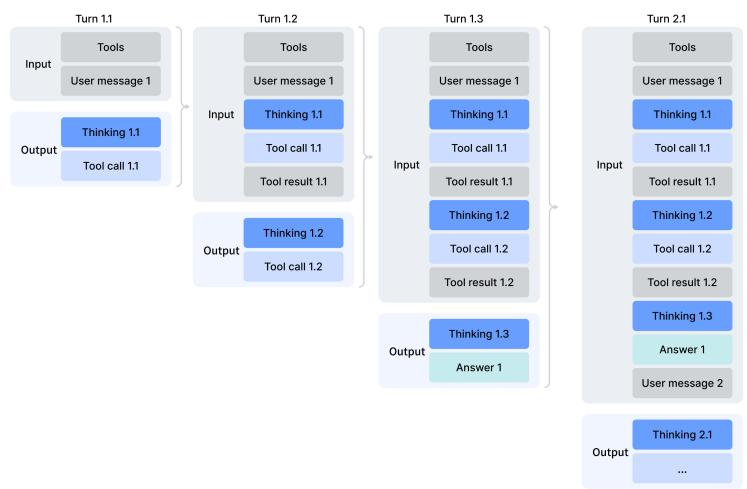
\includegraphics[keepaspectratio,alt={image}]{images/4be752e05d87cef59ec7af493df9496715a6bc784d70c4211ed49472fa3d170a.jpg}}

\begin{enumerate}
\def\labelenumi{\alph{enumi})}
\tightlist
\item
  Thinking with tools
\end{enumerate}

\pandocbounded{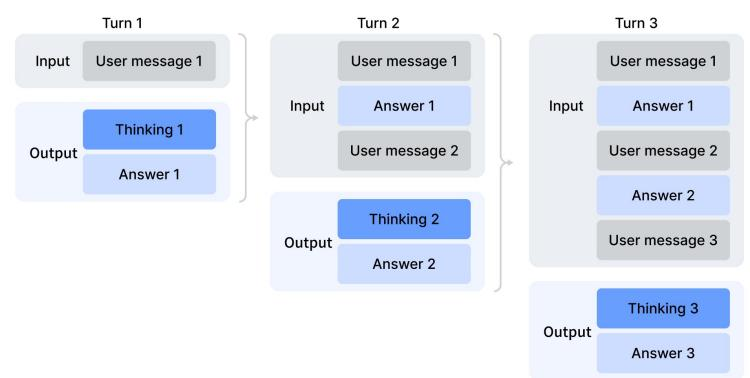
\includegraphics[keepaspectratio,alt={image}]{images/24960dcda89eda0cde433e9ee38d0be1707fe778a521bc2f8fc0b6bf09235192.jpg}}

\begin{enumerate}
\def\labelenumi{\alph{enumi})}
\setcounter{enumi}{1}
\tightlist
\item
  Thinking without tools
\end{enumerate}

Figure 7 \textbar{} Thinking management of DeepSeek-V4 series.

Quick Instruction. In chatbot scenarios, a number of auxiliary tasks
(e.g., determining whetherto trigger a web search, intent recognition,
etc.) must be executed before generating the response.Conventionally,
these tasks are handled by a separate small model, requiring redundant
prefill-ing since it cannot reuse the existing KV cache. To overcome
this limitation, we introduce QuickInstruction. We append a set of
dedicated special tokens directly to the input sequence, whereeach token
corresponds to a specific auxiliary task. By directly reusing the
already-computedKV cache, this mechanism completely avoids redundant
prefilling and allows certain tasks, suchas generating search queries
and determining authority and domain, to be executed in
parallel.Consequently, this approach significantly reduces the
user-perceived time-to-first-token (TTFT)and eliminates the engineering
overhead of maintaining and iterating an extra small model. Thesupported
Quick Instruction tokens are summarized in Table 5.

\section{5.1.2. On-Policy Distillation}\label{on-policy-distillation}

After training multiple domain-specific experts via specialized
fine-tuning and reinforcementlearning, we employ multi-teacher On-Policy
Distillation (OPD) as the primary technique formerging expert
capabilities into the final model. OPD has emerged as an effective
post-trainingparadigm for efficiently transferring the knowledge and
capabilities of domain experts to asingle, unified model. This is
achieved by having the student learn from the output distributionsof
teacher models on its own generated trajectories. Formally, given a set
of \(N\) expert models

Table 5 \textbar{} Quick Instruction special tokens for auxiliary tasks.

{\def\LTcaptype{none} % do not increment counter
\begin{longtable}[]{@{}|l|l|l|@{}}
\toprule\noalign{}
\endhead
\bottomrule\noalign{}
\endlastfoot
\hline
Special Token & Description & Format \\
\hline
\textless\textbar action\textbar\textgreater{} & Determines whether the
user prompt requires a web search or can be answered directly. &
...\textless\textbar User\textbar\textgreater\{prompt\}\textless\textbar Assistant\textbar\textgreater\textless think\textgreater\textless\textbar action\textbar\textgreater{} \\
\hline
\textless\textbar title\textbar\textgreater{} & Generates a concise
conversation title after the first assis-tant response. &
...\textless\textbar Assistant\textbar\textgreater\{response\}\textless\textbar end\_ofsentence\textbar\textgreater\textless\textbar title\textbar\textgreater{} \\
\hline
\textless\textbar query\textbar\textgreater{} & Generates search queries
for the user prompt. &
...\textless\textbar User\textbar\textgreater\{prompt\}\textless\textbar query\textbar\textgreater{} \\
\hline
\textless\textbar authority\textbar\textgreater{} & Classifies the user
prompt\textquotesingle s demand for source authorita-tiveness. &
...\textless\textbar User\textbar\textgreater\{prompt\}\textless\textbar authority\textbar\textgreater{} \\
\hline
\textless\textbar domain\textbar\textgreater{} & Identifies the domain
of the user prompt. &
...\textless\textbar User\textbar\textgreater\{prompt\}\textless\textbar domain\textbar\textgreater{} \\
\hline
\textless\textbar extracted\_url\textbar\textgreater{} & Determines
whether each URL in the user prompt should be fetched and read. &
...\textless\textbar User\textbar\textgreater\{prompt\}\textless\textbar extracted\_url\textbar\textgreater\{url\}\textless\textbar read\_url\textbar\textgreater{} \\
\hline
\end{longtable}
}

\(\{ \pi _ { E _ { 1 } } , \pi _ { E _ { 2 } } , \ldots , \pi _ { E _ { N } } \} ,\)
, the OPD objective function is defined as:

\[
\mathcal {L} _ {\mathrm {O P D}} (\theta) = \sum_ {i = 1} ^ {N} w _ {i} \cdot \mathrm {D} _ {\mathrm {K L}} \left(\pi_ {\theta} \| \pi_ {E _ {i}}\right). \tag {29}
\]

In this formulation, \(w _ { i }\) represents the assigned weight for
each expert, typically determined bythe relative importance of the
expert. Computing the reverse KL loss
\(\operatorname { D } _ { \mathrm { K L } } \left( \pi _ { \theta } \parallel \pi _ { E _ { i } } \right)\)
requiressampling training trajectories from the student
\(\pi _ { \theta }\) to maintain on-policy learning. The underly-ing
logic ensures that the unified policy \(\pi _ { \theta }\) selectively
learns from the specialized expert relevantto the current task context
(e.g., aligning with the mathematics expert for math reasoning tasksand
the coding expert for programming tasks). Through this mechanism, the
knowledge fromphysically distinct expert weights is consolidated into a
unified parameter space via logits-levelalignment, practically
circumventing the performance degradation often encountered in
tra-ditional weight-merging or mixed RL techniques. In this stage, more
than ten teacher modelscovering various domains are employed to distill
a single student model.

In handling the above OPD objective, prior works usually simplify the
full-vocabulary KLloss into a token-level KL estimate at each token
position, and reuse RL framework by replac-ing sg - log ???? ( ??
\textbar{} , \textless?? )???? ( ???? \textbar{} ??,??\textless?? )
\(\begin{array} { r } { \operatorname* { i n g } \operatorname { s g } \bigl [ \log \frac { \pi _ { E _ { i } } ( y _ { t } | x , y _ { < t } ) } { \pi _ { \theta } ( y _ { t } | x , y _ { \le t } ) } \bigr ] } \end{array}\)
(sg represents the stop gradient operation) as the per-token
advantageestimate in the policy loss calculation. Although this approach
is resource-efficient, it leadsto high variance in gradient estimation
and often causes training instability. Therefore, weadopt
full-vocabulary logit distillation in our OPD. Preserving the complete
logit distribution incalculating reverse KL loss yields more stable
gradient estimates and ensures faithful distillationof the teachers'
knowledge. In the following subsection, we describe the engineering
efforts thatmake full-vocabulary OPD feasible at scale.

\section{5.2. RL and OPD
Infrastructures}\label{rl-and-opd-infrastructures}

Our post-training infrastructure is built upon the scalable framework
developed for DeepSeek-V3.2. Specifically, we integrate the same
distributed training stack described in Section 3.5 andthe rollout
engine introduced earlier for efficient auto-regressive sampling.
Building on thisfoundation, we introduce the following principal
enhancements in the present work. Thesedesigns enable efficient
execution of ultra-long-context RL and OPD merging tasks involvingover
ten distinct teacher models, thereby substantially accelerating the
iteration cycle for modelreleases.

\section{5.2.1. FP4 Quantization
Integration}\label{fp4-quantization-integration}

We apply FP4 (MXFP4) quantization to accelerate both rollouts and all
inference-only forwardpasses, including those of teacher and reference
models, thereby reducing memory traffic andsampling latency. As detailed
in Section 3.4, we directly use native FP4 weights during therollout and
inference phases. For training steps, FP4 quantization is simulated via
a losslessFP4-to-FP8 dequantization step, allowing seamless reuse of the
existing FP8 mixed-precisionframework with FP32 master weights and
requiring no modification to the backward pipeline.

\section{5.2.2. Efficient Teacher Scheduling for Full-Vocabulary
OPD}\label{efficient-teacher-scheduling-for-full-vocabulary-opd}

Our framework supports full-vocabulary On-Policy Distillation (OPD) with
an effectivelyunbounded number of teachers, each potentially comprising
trillions of parameters. To enablethis, all teacher weights are
offloaded to a centralized distributed storage and are loaded ondemand
during the teacher forward pass with ZeRO-like parameter sharding to
alleviate bothI/O and DRAM pressure. Furthermore, naively materializing
logits for a vocabulary size\(\vert V \vert > 1 0 0 \mathrm { k }\)
across all teachers is prohibitive, even when spooled to disk. We
address this bycaching only the last-layer teacher hidden states in a
centralized buffer during the forwardpass. At training time, these
cached states are retrieved and passed through the
correspondingprediction head module to reconstruct the full logits on
the fly. This design incurs negligiblerecomputation overhead while
completely circumventing the memory burden associated withexplicit
logits materialization. To mitigate the GPU memory footprint of the
teacher predictionhead, we order training samples by teacher index
during data dispatching. This arrangementensures that each distinct
teacher head is loaded only once per mini-batch and that at mostone
teacher head resides in device memory at any given time. All parameters
and hidden stateloading/offloading operations proceed asynchronously in
the background, without blockingcomputation on the critical path.
Finally, the exact KL divergences between teacher and studentlogits are
computed using a specialized TileLang kernel, which accelerates the
computation andcurtails dynamic memory allocation.

\section{5.2.3. Preemptible and Fault-Tolerant Rollout
Service}\label{preemptible-and-fault-tolerant-rollout-service}

To maximize GPU resource utilization while enabling rapid hardware
provisioning for high-priority tasks, our GPU cluster employs a
cluster-wide preemptive task scheduler, where anyrunning task may be
preempted at any time. Also, hardware failures are prevalent in
large-scaleGPU clusters. To this end, we implement a preemptible and
fault-tolerant LLM generationservice for RL/OPD rollout.

Specifically, we implement a token-granular Write-Ahead Log (WAL) for
each generationrequest. Whenever a new token is generated for a request,
we immediately append it to thatrequest's WAL. During preemption, we
pause the inference engine and save the KV cache of

unfinished requests. Upon resumption, we use the persisted WALs and
saved KV cache tocontinue decoding. Even when a fatal hardware error
occurs, we can re-run the prefill phaseusing the persisted tokens in WAL
to reconstruct the KV cache.

Importantly, it is mathematically incorrect to regenerate unfinished
requests from scratch,as this introduces length bias. Because shorter
responses are more likely to survive interrup-tion, regenerating from
scratch makes the model more prone to producing shorter
sequenceswhenever an interruption occurs. If the inference stack is
batch-invariant and deterministic,this correctness issue could also be
addressed by regenerating with a consistent seed for thepseudorandom
number generator used in the sampler. However, this approach still
incurs theextra cost of re-running the decoding phase, making it far
less efficient than our token-granularWAL method.

\section{5.2.4. Scaling RL Framework for Million-Token
Context}\label{scaling-rl-framework-for-million-token-context}

We introduce targeted optimizations for efficient RL and OPD on
million-token sequences.During the rollout phase, we adopt a preemptible
and fault-tolerant rollout service, detailed inSection 5.2.3. For the
inference and training phase, we decompose the rollout data format
intolightweight metadata and heavy per-token fields. During data
dispatching, the metadata for theentire rollout data can be loaded to
perform global shuffling and packing layout computation.Heavy per-token
fields are loaded via a shared-memory data loader to eliminate
intra-nodedata redundancy and are released immediately upon consumption
at the mini-batch granularity,substantially reducing both CPU and GPU
memory pressure. The number of on-device mini-batches is dynamically
determined based on workload, allowing an efficient trade-off
betweencomputational throughput and I/O overlap.

\section{5.2.5. Sandbox Infrastructure for Agentic
AI}\label{sandbox-infrastructure-for-agentic-ai}

To meet the diverse execution demands of agentic AI during post-training
and evaluation,we build a production-grade sandbox platform, DeepSeek
Elastic Compute (DSec). DSeccomprises three Rust components --- the API
gateway (Apiserver), per-host agent (Edge), andthe cluster monitor
(Watcher) --- that are interconnected by a custom RPC protocol and
scalehorizontally atop the 3FS distributed filesystem (DeepSeek-AI,
2025). In production, a singleDSec cluster manages hundreds of thousands
of concurrent sandbox instances.

The design of DSec is motivated by four observations: (1) agentic
workloads are highlyheterogeneous, spanning lightweight function calls
to full software-engineering pipelines withdiverse OS and security
requirements; (2) environment images are numerous and large, yet
mustload quickly and support iterative customization; (3) high-density
deployment demands efficientCPU and memory utilization; (4) sandbox
lifecycles must coordinate with GPU training sched-ules, including
preemption and checkpoint-based resumption. Based on these observations,
weelaborate on the four core designs of DSec individually in the
following.

Four Execution Substrates Behind One Unified Interface. DSec exposes a
single PythonSDK (libdsec) that abstracts four execution substrates.
Function Call dispatches statelessinvocations to a pre-warmed container
pool, eliminating cold-start overhead. Container is
fullyDocker-compatible and leverages EROFS (Gao et al., 2019) on-demand
loading for efficientimage assembly. microVM, built on Firecracker
(Agache et al., 2020), adds VM-level isolation forsecurity-sensitive,
high-density deployments. fullVM, built on QEMU (Bellard, 2005),
supportsarbitrary guest operating systems. All four share a common API
surface --- command execution,

file transfer, and TTY access --- and switching between them requires
only a parameter change.

Fast Image Loading via Layered Storage. DSec reconciles fast startup
with a large and growingcorpus of environment images through layered,
on-demand loading. For containers, base imagesand filesystem commits are
stored as 3FS-backed readonly EROFS layers mounted directly intooverlay
lowerdirs. We keep file metadata readily available on the local disk at
mount time;meanwhile, data blocks are fetched from 3FS upon request. For
microVMs, DSec uses theoverlaybd (Li et al., 2020) disk format: the
read-only base layer resides on 3FS for cross-instance sharing, while
writes go to a local copy-on-write layer. Such snapshots are
chainable,facilitating efficient versioning and millisecond-scale
resumption.

Density Optimizations Under Massive Concurrency. To accommodate hundreds
of thousandsof sandboxes per cluster, DSec tackles two resource
bottlenecks. First, it mitigates duplicatepage-cache footprints in
virtualized environments and applies memory reclamation to enablesafe
overcommitment. Second, it alleviates spinlock contention in the
container runtime andtherefore, reduces per-sandbox CPU overhead,
significantly increasing per-host packing density.

Trajectory Logging and Preemption-Safe Resumption. DSec maintains a
globally orderedtrajectory log for each sandbox, persistently recording
every command invocation and its results.The trajectory serves three
purposes: (1) client fast-forwarding --- when a training task
ispreempted, sandbox resources are retained nonetheless; upon
resumption, DSec replays cachedresults for previously completed
commands, accelerating task recovery whilst also preventingerrors from
re-execution of non-idempotent operations; (2) fine-grained provenance
--- theorigin and corresponding outcomes of each state change are
traceable; (3) deterministic replay--- any historical session can be
faithfully reproduced from its trajectory.

\section{5.3. Standard Benchmark
Evaluation}\label{standard-benchmark-evaluation}

\section{5.3.1. Evaluation Setup}\label{evaluation-setup}

Knowledge and Reasoning. Knowledge and reasoning datasets include
MMLU-Pro (Wanget al., 2024b), GPQA (Rein et al., 2023), Human Last Exam
(Phan et al., 2025), Simple-QA Veri-fied (Haas et al., 2025),
Chinese-SimpleQA (He et al., 2024), LiveCodeBench-v6 (Jain et al.,
2024),CodeForces (Internal Benchmark), HMMT 2026 Feb, Apex (Balunovi´c
et al., 2025), Apex Short-list (Balunovi´c et al., 2025), IMOAnswerBench
(Luong et al., 2025), and PutnamBench (Tsoukalaset al., 2024).

For code, we evaluate DeepSeek-V4 series on LiveCodeBench-v6 and an
internal Codeforcesbenchmark. For Codeforces, we collect 14 Codeforces
Division 1 contests comprising 114problems (May 2025 - November 2025).
The Elo rating is computed as follows. For each contest,we generate 32
candidate solutions per problem. For each problem independently, we
sample10 of these solutions without replacement and arrange them in a
random order to form thesubmission sequence. Each submission is judged
against a test suite constructed by domainexperts. The score for a
solved problem follows the penalty scheme of OpenAI (2025): the
modelreceives the median score of human participants who solved the same
problem with the samenumber of prior failed attempts. This yields a
total contest score for each sampled submissionsequence, which is then
converted into a contest rank and subsequently into an estimated
ratingvia the standard Codeforces rating system. The contest-level
expected rating is defined as the

expectation of this estimated rating over all possible random selections
and orderings of the10 submissions per problem. The model's overall
rating is the average of these contest-levelexpected ratings across all
14 contests.

For reasoning and knowledge tasks, we set the temperature to 1.0 and the
context window to8K, 128K, and 384K tokens for the Non-think, High, and
Max modes, respectively. For math tasks(e.g., HMMT, IMOAnswerBench,
Apex, and HLE), we evaluate using the following
template:``\{question\}\nPlease reason step by step, and put your final
answer within\boxed{}.'' For DeepSeek-V4-Pro-Max on math tasks, we use
the following template to elicitdeeper reasoning: ``Solve the following
problem. The problem may ask you toprove a statement, or ask for an
answer. If finding an answer is required,you should come up with the
answer, and your final solution should also bea rigorous proof of that
answer being valid.\n\n{question}''.

For formal math tasks, we evaluate in an agentic setting on Lean
v4.28.0-rc1 (Moura andUllrich, 2021), with access to the Lean compiler
and a semantic tactic search engine, runningup to 500 tool calls with
max reasoning effort. In addition, we evaluate a more compute-intensive
pipeline in which candidate natural-language solutions are first
generated and filteredby self-verification(Shao et al., 2025), and the
retained solutions are then provided as guidanceto a formal agent for
proving the corresponding Lean statement. This design uses
informalreasoning to improve exploration while preserving strict
correctness through formal verification.A submission is counted as
correct only if the strict verifier Comparator accepts it for
bothsettings.

We have left some entries blank for K2.6 and GLM-5.1, as their APIs were
too busy to returnresponses to our queries.

1M-Token Context. Since DeepSeek-V4 series supports 1M-token contexts,
we evaluate modelperformance in a long context scenario by selecting
OpenAI MRCR (OpenAI, 2024b) andCorpusQA (Lu et al., 2026) as the
benchmarks. We re-evaluate Claude Opus 4.6 and Gemini 3.1Pro on these
tasks with the goal of standardizing the configuration across all
models. We didnot evaluate GPT-5.4 because its API failed to respond to
a large portion of our queries.

Agent. Agent datasets include Terminal Bench 2.0 (Merrill et al., 2026),
SWE-Verified (OpenAI,2024e), SWE Multilingual (Yang et al., 2025),
SWE-Pro (Deng et al., 2025), BrowseComp (Weiet al., 2025), the public
evaluation set of MCPAtlas (Bandi et al., 2026), GDPval-AA (AA,
2025;Patwardhan et al., 2025), and Tool-Decathlon (Li et al., 2025).

For code agent tasks (SWE-Verified, Terminal-Bench, SWE-Pro, SWE
Multilingual), we eval-uate DeepSeek-V4 series using an internally
developed evaluation framework. This frameworkprovides a minimal set of
tools --- a bash tool and a file-edit tool. The maximum number
ofinteraction steps is set to 500, and the maximum context length is set
to 512K tokens. RegardingTerminal-Bench 2.0, we acknowledge the
environment-related issues noted by GLM-5.1. Never-theless, we report
our performance on the original Terminal-Bench 2.0 dataset for
consistency.On the Terminal-Bench 2.0 Verified subset, DeepSeek-V4-Pro
achieves a score of approximately72.0.

For search agent tasks (BrowseComp, HLE w/ tool), we also use an
in-house harness withwebsearch and Python tool, and set maximum
interaction steps to 500 and the maximum contextlength to 512K tokens.
For BrowseComp, we use the same discard-all context managementstrategy
as DeepSeek-V3.2 (DeepSeek-AI, 2025).

\section{5.3.2. Evaluation Results}\label{evaluation-results-1}

Table 6 \textbar{} Comparison between DeepSeek-V4-Pro-Max and
closed/open source models. ``Max'',``xHigh'', and ``High'' denote
reasoning effort. The best results are highlighted in bold;
thesecond-best results are underlined.

{\def\LTcaptype{none} % do not increment counter
\begin{longtable}[]{@{}llllllll@{}}
\toprule\noalign{}
\endhead
\bottomrule\noalign{}
\endlastfoot
\multicolumn{2}{@{}l}{%
Benchmark (Metric)} & Opus-4.6 Max & GPT-5.4 xHigh & Gemini-3.1-Pro High
& K2.6 Thinking & GLM-5.1 Thinking & DS-V4-Pro Max \\
\multirow{11}{*}{Knowledge \& Reasoning} & MMLU-Pro (EM) & 89.1 & 87.5 &
91.0 & 87.1 & 86.0 & 87.5 \\
& SimpleQA-Verified (Pass@1) & 46.2 & 45.3 & 75.6 & 36.9 & 38.1 &
57.9 \\
& Chinese-SimpleQA (Pass@1) & 76.4 & 76.8 & 85.9 & 75.9 & 75.0 & 84.4 \\
& GPQA Diamond (Pass@1) & 91.3 & 93.0 & 94.3 & 90.5 & 86.2 & 90.1 \\
& HLE (Pass@1) & 40.0 & 39.8 & 44.4 & 36.4 & 34.7 & 37.7 \\
& LiveCodeBench (Pass@1) & 88.8 & - & 91.7 & 89.6 & - & 93.5 \\
& Codeforces (Rating) & - & 3168 & 3052 & - & - & 3206 \\
& HMMT 2026 Feb (Pass@1) & 96.2 & 97.7 & 94.7 & 92.7 & 89.4 & 95.2 \\
& IMOAnswerBench (Pass@1) & 75.3 & 91.4 & 81.0 & 86.0 & 83.8 & 89.8 \\
& Apex (Pass@1) & 34.5 & 54.1 & 60.9 & 24.0 & 11.5 & 38.3 \\
& Apex Shortlist (Pass@1) & 85.9 & 78.1 & 89.1 & 75.5 & 72.4 & 90.2 \\
\multirow{2}{*}{Long} & MRCR 1M (MMR) & 92.9 & - & 76.3 & - & - &
83.5 \\
& CorpusQA 1M (ACC) & 71.7 & - & 53.8 & - & - & 62.0 \\
\multirow{9}{*}{Agentic} & Terminal Bench 2.0 (Acc) & 65.4 & 75.1 & 68.5
& 66.7 & 63.5 & 67.9 \\
& SWE Verified (Resolved) & 80.8 & - & 80.6 & 80.2 & - & 80.6 \\
& SWE Pro (Resolved) & 57.3 & 57.7 & 54.2 & 58.6 & 58.4 & 55.4 \\
& SWE Multilingual (Resolved) & 77.5 & - & - & 76.7 & 73.3 & 76.2 \\
& BrowseComp (Pass@1) & 83.7 & 82.7 & 85.9 & 83.2 & 79.3 & 83.4 \\
& HLE w/ tools (Pass@1) & 53.1 & 52.0 & 51.6 & 54.0 & 50.4 & 48.2 \\
& GDPval-AA (Elo) & 1619 & 1674 & 1314 & 1482 & 1535 & 1554 \\
& MCPAtlas Public(Pass@1) & 73.8 & 67.2 & 69.2 & 66.6 & 71.8 & 73.6 \\
& Toolathlon (Pass@1) & 47.2 & 54.6 & 48.8 & 50.0 & 40.7 & 51.8 \\
\end{longtable}
}

The comparison of DeepSeek-V4-Pro-Max and other closed/open source
models is presentedin Table 6. Also, we evaluate different modes of
DeepSeek-V4-Flash and DeepSeek-V4-Pro andshow the results in Table 7.

Knowledge. In the evaluation of general world knowledge,
DeepSeek-V4-Pro-Max, the max-imum reasoning effort mode of
DeepSeek-V4-Pro, establishes a new state-of-the-art amongopen-source
large language models. As demonstrated by the SimpleQA-Verified,
DeepSeek-V4-Pro-Max significantly outperforms all existing open-source
baselines by a margin of 20 absolutepercentage points. Despite these
advances, it currently trails the leading proprietary
model,Gemini-3.1-Pro. In the domain of educational knowledge and
reasoning, DeepSeek-V4-Pro-Maxmarginally outperforms Kimi and GLM across
the MMLU-Pro, GPQA, and HLE benchmarks,although it lags behind leading
proprietary models. Broadly, DeepSeek-V4-Pro-Max marks asignificant
milestone in enhancing the world knowledge capabilities of open-source
models.

In addition, a significant performance gap exists between
DeepSeek-V4-Flash and DeepSeek-V4-Pro on knowledge-based tasks; this is
anticipated, as larger parameter counts facilitategreater knowledge
retention during pre-training. Notably, both models demonstrate
improvedresults on knowledge benchmarks when allocated higher reasoning
effort.

Table 7 \textbar{} Comparison among different sizes and modes of
DeepSeek-V4 series. ``Non-Think'',``High'', and ``Max'' denote reasoning
effort.

{\def\LTcaptype{none} % do not increment counter
\begin{longtable}[]{@{}llllllll@{}}
\toprule\noalign{}
\endhead
\bottomrule\noalign{}
\endlastfoot
\multirow{2}{*}{} & \multirow{2}{*}{Benchmark (Metric)} &
\multicolumn{3}{l}{%
DeepSeek-V4-Flash} & \multicolumn{3}{l@{}}{%
DeepSeek-V4-Pro} \\
& & Non-Think & High & Max & Non-Think & High & Max \\
\multirow{11}{*}{Knowledge \& Reasoning} & MMLU-Pro (EM) & 83.0 & 86.4 &
86.2 & 82.9 & 87.1 & 87.5 \\
& SimpleQA-Verified (Pass@1) & 23.1 & 28.9 & 34.1 & 45.0 & 46.2 &
57.9 \\
& Chinese-SimpleQA (Pass@1) & 71.5 & 73.2 & 78.9 & 75.8 & 77.7 & 84.4 \\
& GPQA Diamond (Pass@1) & 71.2 & 87.4 & 88.1 & 72.9 & 89.1 & 90.1 \\
& HLE (Pass@1) & 8.1 & 29.4 & 34.8 & 7.7 & 34.5 & 37.7 \\
& LiveCodeBench (Pass@1-COT) & 55.2 & 88.4 & 91.6 & 56.8 & 89.8 &
93.5 \\
& Codeforces (Rating) & - & 2816 & 3052 & - & 2919 & 3206 \\
& HMMT 2026 Feb (Pass@1) & 40.8 & 91.9 & 94.8 & 31.7 & 94.0 & 95.2 \\
& IMOAnswerBench (Pass@1) & 41.9 & 85.1 & 88.4 & 35.3 & 88.0 & 89.8 \\
& Apex (Pass@1) & 1.0 & 19.1 & 33.0 & 0.4 & 27.4 & 38.3 \\
& Apex Shortlist (Pass@1) & 9.3 & 72.1 & 85.7 & 9.2 & 85.5 & 90.2 \\
\multirow{2}{*}{Long} & MRCR 1M(MMR) & 37.5 & 76.9 & 78.7 & 44.7 & 83.3
& 83.5 \\
& CorpusQA 1M(ACC) & 15.5 & 59.3 & 60.5 & 35.6 & 56.5 & 62.0 \\
\multirow{9}{*}{Agentic} & Terminal Bench 2.0 (Acc) & 49.1 & 56.6 & 56.9
& 59.1 & 63.3 & 67.9 \\
& SWE Verified (Resolved) & 73.7 & 78.6 & 79.0 & 73.6 & 79.4 & 80.6 \\
& SWE Pro (Resolved) & 49.1 & 52.3 & 52.6 & 52.1 & 54.4 & 55.4 \\
& SWE Multilingual (Resolved) & 69.7 & 70.2 & 73.3 & 69.8 & 74.1 &
76.2 \\
& BrowseComp (Pass@1) & - & 53.5 & 73.2 & - & 80.4 & 83.4 \\
& HLE w/ tools (Pass@1) & - & 40.3 & 45.1 & - & 44.7 & 48.2 \\
& MCPAtlas Public (Pass@1) & 64.0 & 67.4 & 69.0 & 69.4 & 74.2 & 73.6 \\
& GDPval-AA (Elo) & - & - & 1395 & - & - & 1554 \\
& Toolathlon (Pass@1) & 40.7 & 43.5 & 47.8 & 46.3 & 49.0 & 51.8 \\
\end{longtable}
}

Reasoning. DeepSeek-V4-Pro-Max outperforms all prior open models across
reasoning bench-marks, and matches state-of-the-art closed models on
many metrics, while the smaller DeepSeek-V4-Flash-Max also surpasses the
previous best open-source model, K2.6-Thinking, on codeand math
reasoning tasks. Meanwhile, DeepSeek-V4-Pro and DeepSeek-V4-Flash excel
in cod-ing competitions. According to our evaluation, their performance
is comparable to GPT-5.4,making this the first time an open model has
matched a closed model on this task. On theCodeforces leaderboard,
DeepSeek-V4-Pro-Max currently ranks 23rd among human
candidates.DeepSeek-V4 also demonstrates strong performance on formal
mathematical task under bothagentic and compute-intensive settings.
Under an agentic setup, it achieves state-of-the-artresults, shown in
Figure 8, outperforming prior models such as Seed Prover (Chen et al.,
2025).With a more compute-intensive pipeline, performance further
improves, surpassing systemsincluding Aristotle(Achim et al., 2025) and
matching the best known results under this setting.

Agent. The DeepSeek-V4 series demonstrates strong agent performance in
evaluations. Forcode agent tasks, DeepSeek-V4-Pro achieves results
comparable to K2.6 and GLM-5.1, thoughall these open models still lag
behind their closed-source counterparts. DeepSeek-V4-Flashunderperforms
DeepSeek-V4-Pro on coding tasks, particularly on Terminal Bench 2.0. A
similartrend is observed across other agent evaluations. It is worth
noting that DeepSeek-V4-Properforms well on MCPAtlas and
Toolathlon---two evaluation test sets that include a wide rangeof tools
and MCP services---indicating that our model has excellent
generalization capabilityand does not perform well only on internal
frameworks.

Practical RegimePutnam-200 Pass@8 with minimal toolsand bounded
sampling.

\pandocbounded{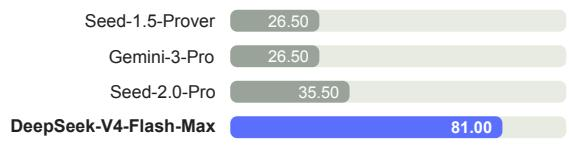
\includegraphics[keepaspectratio,alt={image}]{images/033e143b8217ed1d5ac9c328c9993ffd61514d8e04df84d9320917cc51238dfa.jpg}}

Frontier RegimePutnam-2025 with hybrid formal-informalreasoning and
substantial compute scaling.

\pandocbounded{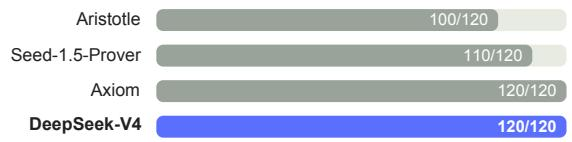
\includegraphics[keepaspectratio,alt={image}]{images/01305727e84924cb89df98d0699b8d023302eadc02fe675342c2cfd1cee0f6b5.jpg}}

Figure 8 \textbar{} Formal reasoning under practical and frontier
regimes. Left: Putnam-200 Pass@8evaluates a fixed random subset of
PutnamBench (Tsoukalas et al., 2024) following the setupintroduced by
Seed-Prover; all models are tested on the same problem set. We follow
the Seed-Prover protocol but replace proprietary search tools with the
open-source LeanExplore (Asher,2025), yielding a lightweight setting
with minimal agent tools and bounded sampling. Right:Putnam-2025 probes
the frontier of mathematical reasoning in a scaled hybrid
formal-informalregime, where informal reasoning is combined with formal
verification to expose gaps andimprove rigor; DeepSeek-V4 reaches a
proof-perfect 120/120.

\pandocbounded{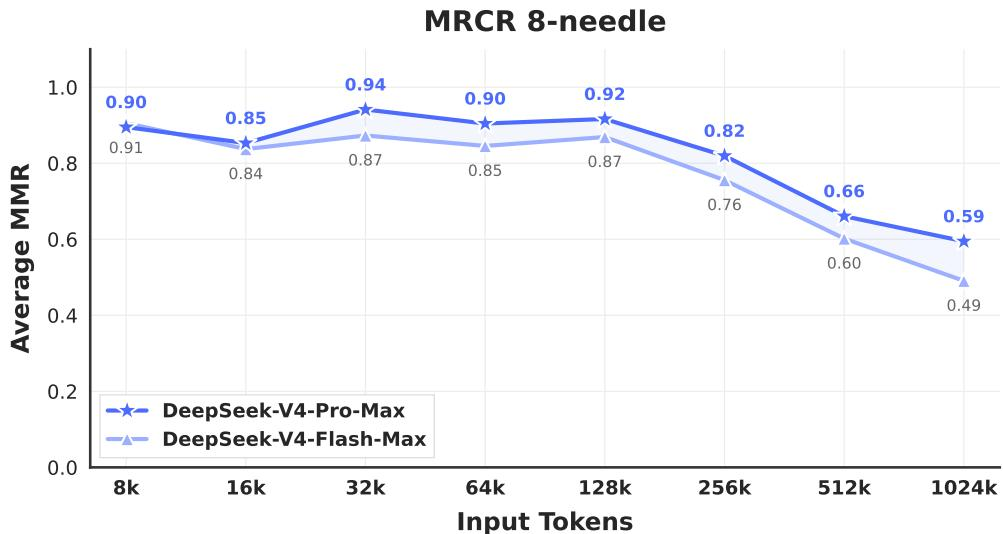
\includegraphics[keepaspectratio,alt={image}]{images/a7065923549538da2b7d0ead2a01c83fbbad9968a5da8a07efdb572247e4f193.jpg}}

Figure 9 \textbar{} DeepSeek-V4 series performance on the MRCR task.

1M-Token Context. DeepSeek-V4-Pro outperforms Gemini-3.1-Pro on the MRCR
task, whichmeasures in-context retrieval, but remains behind Claude Opus
4.6. As illustrated in Figure 9,retrieval performance remains highly
stable within a 128K context window. While a performancedegradation
becomes visible beyond the 128K mark, the model's retrieval capabilities
at 1Mtokens remain remarkably strong compared to both proprietary and
open-source counterparts.Unlike MRCR, CorpusQA is similar to real
scenarios. The evaluation results also indicate thatDeepSeek-V4-Pro is
better than Gemini-3.1-Pro.

Reasoning Effort. As shown in Table 7, the Max mode, which employs
longer contexts andreduced length penalties in \({ \mathrm { R L } } ,\)
outperforms the High mode on the most challenging tasks.Figure 10
presents a comparison of performance and cost among DeepSeek-V4-Pro,
DeepSeek-V4-Flash, and DeepSeek-V3.2 on representative reasoning and
agentic tasks. By scaling test-timecompute, DeepSeek-V4 series achieve
substantial improvements over the predecessor. Further-more, on
reasoning tasks like HLE, DeepSeek-V4-Pro demonstrates higher token
efficiency than

\pandocbounded{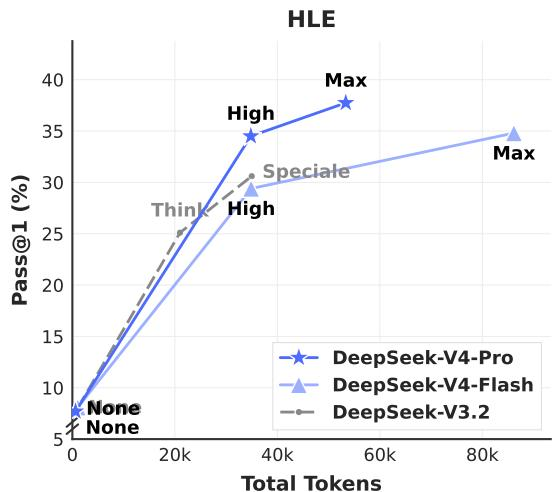
\includegraphics[keepaspectratio,alt={image}]{images/253b09ee67a4e46163ee468aa73d814efa6f7583bcfb245ba2971937515544b3.jpg}}

\pandocbounded{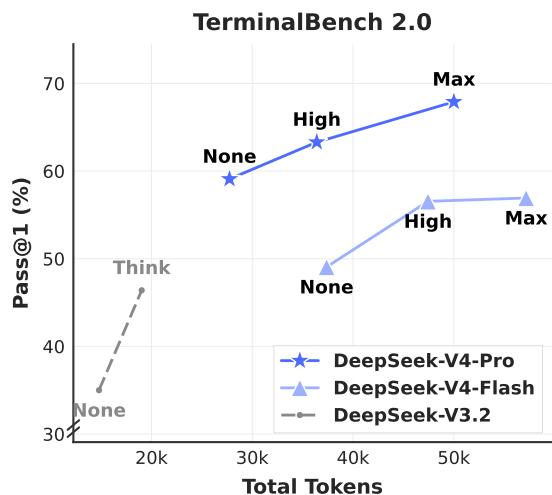
\includegraphics[keepaspectratio,alt={image}]{images/610e79b834f385384649cf97fe6162ed2c0e51a46557b9913a0d08cd823db490.jpg}}

Figure 10 \textbar{} HLE and Terminal Bench 2.0 performance by reasoning
effort. ``None'' indicatesNon-think mode, and ``Speciale'' indicates
DeepSeek-V3.2-Speciale model.

DeepSeek-V3.2.

\section{5.4. Performance on Real-World
Tasks}\label{performance-on-real-world-tasks}

Standardized benchmarks often struggle to capture the complexities of
diverse, real-worldtasks, creating a gap between test results and actual
user experience. To bridge this, we havedeveloped proprietary internal
metrics that prioritize real-world usage patterns over
traditionalbenchmarks. This approach ensures that our optimizations
translate into tangible benefits.Our evaluation framework specifically
targets the primary use cases of the DeepSeek API andChatbot, aligning
model performance with practical demands.

\section{5.4.1. Chinese Writing}\label{chinese-writing}

One of the primary use cases for DeepSeek is Chinese writing. We
conducted a rigorousevaluation on functional writing and creative
writing. Table 12 presents a pairwise comparisonbetween DeepSeek-V4-Pro
and Gemini-3.1-Pro on functional writing tasks. These tasks consistof
common daily writing queries, where prompts are typically concise and
straightforward.Gemini-3.1-Pro was selected as the baseline, as it
stands as the top-performing external modelfor Chinese writing in our
evaluations. The results indicate that DeepSeek-V4-Pro outperformsthe
baseline with an overall win rate of \(6 2 . 7 \%\) versus
\(3 4 . 1 \%\) ; this is primarily because Geminioccasionally allows its
inherent stylistic preferences to override the user's explicit
requirementsin Chinese writing scenarios.

Table 13 presents the creative writing comparison, which is evaluated
along two axes:instruction following and writing quality. Compared with
Gemini-3.1-Pro, DeepSeek-V4-Proachieves a \(6 0 . 0 \%\) win rate in
instruction following and \(7 7 . 5 \%\) in writing quality,
demonstratinga marginal improvement in instruction following and a
substantial gain in writing quality.Although DeepSeek-V4-Pro yields
superior results in aggregate user case analysis, an
evaluationrestricted to the most challenging prompts --- specifically
those involving high-complexityconstraints or multi-turn scenarios ---
reveals that Claude Opus 4.5 retains a performanceadvantage over
DeepSeek-V4-Pro. As shown in Table 14, Claude Opus 4.5 achieves a
\(5 2 . 0 \%\) winrate versus \(4 5 . 9 \%\) .

\section{5.4.2. Search}\label{search}

Search-augmented question answering is a core capability of the DeepSeek
chatbot. On theDeepSeek web and app, the ``non-think'' mode employs
Retrieval-Augmented Search (RAG),whereas the ``thinking'' mode utilizes
agentic search.

Retrieval Augmented Search. We conducted a pairwise evaluation comparing
DeepSeek-V4-Pro and DeepSeek-V3.2 across both objective and subjective
Q\&A categories. As presented inTable 11, DeepSeek-V4-Pro outperforms
DeepSeek-V3.2 by a substantial margin, demonstratinga consistent
advantage across both categories. The most pronounced gains are observed
insingle-value search and planning \& strategy tasks, suggesting that
DeepSeek-V4-Pro excelsat locating precise factual answers and
synthesizing structured plans from retrieved context.However,
DeepSeek-V3.2 remains relatively competitive on comparison and
recommendationtasks, indicating potential room for improvement for
DeepSeek-V4-Pro in scenarios requiringbalanced, multi-perspective
reasoning over search results.

Agentic Search. Unlike standard RAG, agentic search empowers the model
to iterativelyinvoke search and fetch tools per query, significantly
enhancing overall search performance. Forthe thinking mode in
DeepSeek-Chat, we optimized the agentic search function to
maximizeresponse accuracy within a predefined ``thinking budget''. As
shown in Table 9, agentic searchconsistently outperforms RAG,
particularly on complex tasks. Furthermore, its cost remainshighly
efficient, with agentic search being only marginally more expensive than
standard RAG(see Table 10).

\section{5.4.3. White-Collar Task}\label{white-collar-task}

To rigorously evaluate the model's utility in sophisticated enterprise
productivity scenarios, weconstructed a comprehensive suite of 30
advanced Chinese professional tasks. These workflowsdeliberately
encompass high-level cognitive demands, including in-depth information
analysis,comprehensive document generation, and nuanced document
editing, spanning a diversespectrum of 13 critical industries (e.g.,
finance, education, law, and technology). The evaluationwas conducted
within an in-house agent harness equipped with basic tools, including
Bash andweb search.

Given the open-ended nature of these tasks, automated metrics usually
fall short in capturingthe nuances of a high-quality response.
Therefore, we conducted human evaluations to comparethe performance of
DeepSeek-V4-Pro-Max against Opus-4.6-Max. Annotators blindly assessedthe
model outputs across four dimensions:

• Task Completion: Whether the core problem was successfully resolved.

• Instruction Following: Adherence to specific constraints and
directives.

• Content Quality: Factual accuracy, logical coherence, and professional
tone.

• Formatting Aesthetics: Layout readability and visual presentation.

As illustrated in Figure 11, DeepSeek-V4-Pro-Max outperforms
Opus-4.6-Max on diverseChinese white-collar tasks, achieving an
impressive non-loss rate of \(6 3 \%\) , and demonstratingconsistent
advantages across analysis, generation, and editing tasks. The detailed
dimensionscores shown in Figure 12 highlight the model's primary
strengths in Task Completion and

Content Quality. Specifically, DeepSeek-V4-Pro-Max proactively
anticipates implicit user in-tents by frequently providing supplementary
insights and self-verification steps. It also excelsin long-form
generation, delivering in-depth, coherent narratives rather than relying
on theoverly simplistic bullet points frequently produced by
Opus-4.6-Max. Additionally, the modelstrictly conforms to formal
professional conventions, such as standardized Chinese
hierarchicalnumbering. However, in terms of Instruction Following, it
occasionally overlooks specificformatting constraints and slightly
trails Opus. Furthermore, the model is less proficient atcondensing
extensive text inputs into succinct summaries. Finally, its Formatting
Aestheticsstill have substantial room for improvement regarding the
overall visual design of presentationslides. Figure 13, 14, and 15
present several test cases; due to the extensive length of
certainoutputs, only partial pages are displayed.

\pandocbounded{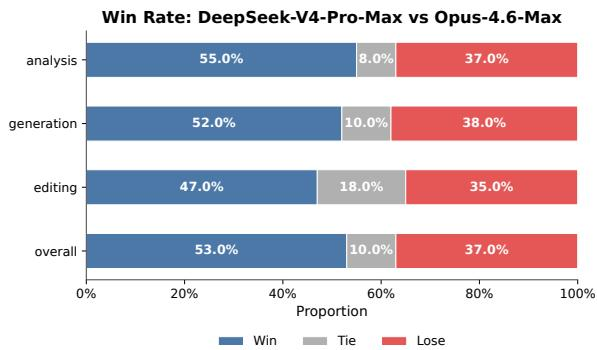
\includegraphics[keepaspectratio,alt={image}]{images/950350f9d0e4720871106117e975590257a0dc0d7b91dfd7f082f7ae73bf717d.jpg}}

Figure 11 \textbar{} Win-rate comparison across analy-sis, generation,
editing tasks, and the overallperformance.

\pandocbounded{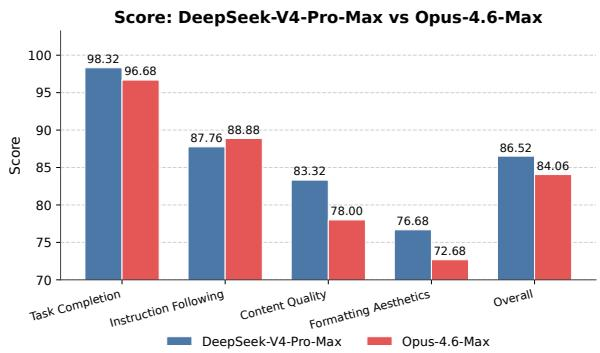
\includegraphics[keepaspectratio,alt={image}]{images/1e3ce11719ce0f4f4fff751f62a32e1bc409b360e1a143e0205e6cb2a80dc98d.jpg}}

Figure 12 \textbar{} Detailed dimension scores includ-ing Task
Completion, Content Quality, Format-ting Aesthetics, and Instruction
Following.

\pandocbounded{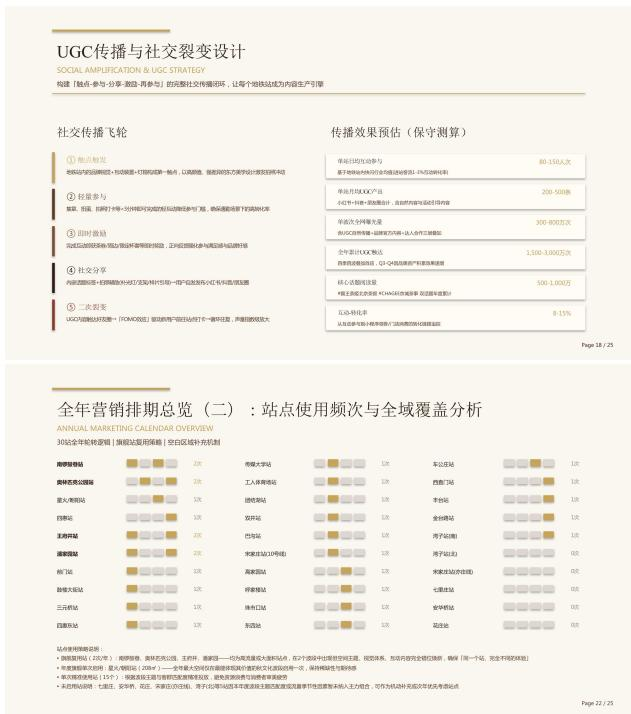
\includegraphics[keepaspectratio,alt={image}]{images/9e26dfa1a5b969aa0ad1e3954a0003685e7a8e4257e5c4850e66ac3db8bd65e7.jpg}}

\pandocbounded{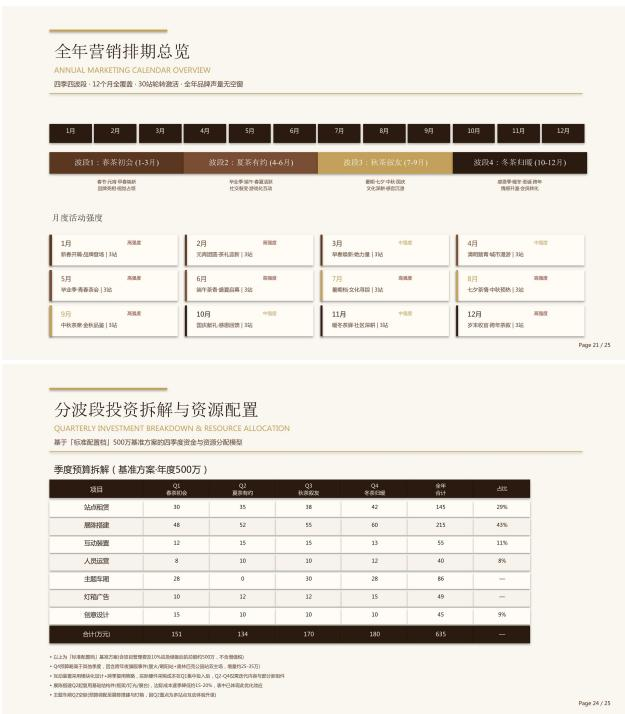
\includegraphics[keepaspectratio,alt={image}]{images/9d70ed5a9b53ac2dbfb1c011b88257ce21004760efc9459ae1df5ed29b9b69a9.jpg}}

Figure 13 \textbar{} Example output of a task which requires drafting a
joint marketing proposal for apopular bubble tea brand and the Beijing
Subway.

\section{5.4.4. Code Agent}\label{code-agent}

To benchmark our coding agent capability, we curate tasks from real
internal R\&D workloadsWe collect \({ \sim } 2 0 0\) challenging tasks
from \(5 0 +\) internal engineers, spanning feature development,bug
fixing, refactoring, and diagnostics across diverse technology stacks
including PyTorch,CUDA, Rust, and \({ { C + + } }\) . Each task is
accompanied by its original repository, the correspondingexecution
environment, and human-annotated scoring rubrics; after rigorous quality
filtering,30 tasks are retained as the evaluation set. As shown in Table
8, DeepSeek-V4-Pro significantlyoutperforms Claude Sonnet 4.5 and
approaches the level of Claude Opus 4.5.

Table 8 \textbar{} Comparison on R\&D Coding Benchmark (external models
included strictly for evalua-tion purposes).

{\def\LTcaptype{none} % do not increment counter
\begin{longtable}[]{@{}|l|l|l|l|l|l|l|@{}}
\toprule\noalign{}
\endhead
\bottomrule\noalign{}
\endlastfoot
\hline
Model & Haiku 4.5 & Sonnet 4.5 & DeepSeek-V4-Pro-Max & Opus 4.5 & Opus
4.5 Thinking & Opus 4.6 Thinking \\
\hline
Pass Rate (\%) & 13 & 47 & 67 & 70 & 73 & 80 \\
\hline
\end{longtable}
}

In a survey asking DeepSeek developers and researchers \(( N = 8 5 )\) )
--- all with experience ofusing DeepSeek-V4-Pro for agentic coding in
their daily work --- whether DeepSeek-V4-Pro isready to serve as their
default and primary coding model compared to other frontier models,
\(5 2 \%\)said yes, \(3 9 \%\) leaned toward yes, and fewer than
\(9 \%\) said no. Respondents find DeepSeek-V4-Proto deliver
satisfactory results across most tasks, but note trivial mistakes,
misinterpretation ofvague prompts, and occasional over-thinking.

\section{6. Conclusion, Limitations, and Future
Directions}\label{conclusion-limitations-and-future-directions}

In this work, we present a preview version of DeepSeek-V4 series, aiming
at next-generationlarge language models that break the efficiency
barrier of ultra-long-context processing. By com-bining a hybrid
attention architecture that integrates CSA and HCA, DeepSeek-V4 series
achievea dramatic leap in long-sequence efficiency. The architectural
innovations, together with exten-sive infrastructure optimization,
enable efficient native support for million-token contexts andestablish
a necessary foundation for future test-time scaling, long-horizon tasks,
and emergingparadigms such as online learning. Evaluation results
demonstrate that DeepSeek-V4-Pro-Max,the maximum reasoning effort mode
of DeepSeek-V4-Pro, redefines the state-of-the-art for openmodels. It
substantially outperforms prior open-source models on knowledge
benchmarks,achieves superior reasoning performance close to the frontier
proprietary models, and deliverscompetitive agent capabilities.
Meanwhile, DeepSeek-V4-Flash-Max attains comparable reason-ing
performance to leading closed models while maintaining a highly
cost-efficient architecture.We believe DeepSeek-V4 series usher in a new
era of million-length contexts for open modelsand pave the way toward
better efficiency, scale, and intelligence.

In pursuit of extreme long-context efficiency, DeepSeek-V4 series
adopted a bold architec-tural design. To minimize risk, we retained many
preliminarily validated components andtricks, which, while effective,
made the architecture relatively complex. In future iterations,we will
carry out more comprehensive and principled investigations to distill
the architecturedown to its most essential designs, making it more
elegant without sacrificing performance.Meanwhile, although Anticipatory
Routing and SwiGLU Clamping have been proven effectivein mitigating
training instabilities, their underlying principles remain
insufficiently understood.We will actively study foundational problems
on training stability and strengthen internal metricmonitoring, aiming
for a more principled and predictive approach to stable large-scale
training.

In addition, beyond the MoE and sparse attention architecture, we will
also proactively exploremodel sparsity along new dimensions --- such as
more sparse embedding modules (Chenget al., 2026) --- to further improve
computational and memory efficiency without compromisingcapability. We
will also continuously investigate low-latency architectures and system
tech-niques to make long-context deployment and interaction more
responsive. Furthermore, werecognize the importance and practical value
of long-horizon, multi-round agentic tasks, andwill continue to iterate
and explore in this direction. We are also working on
incorporatingmultimodal capabilities to our models. Finally, we are
committed to developing better datacuration and synthesis strategies to
consistently enhance model intelligence, robustness, andpractical
usability across an increasingly broad range of scenarios and tasks.

\section{References}\label{references}

AA. Gdpval-aa leaderboard, 2025. URL
https://artificialanalysis.ai/methodology/intelligence-benchmarking\#gdpval-aa.

T. Achim, A. Best, A. Bietti, K. Der, M. Fédérico, S. Gukov, D.
Halpern-Leistner, K. Henningsgard,Y. Kudryashov, A. Meiburg, et
al.~Aristotle: Imo-level automated theorem proving. arXivpreprint
arXiv:2510.01346, 2025.

A. Agache, M. Brooker, A. Florescu, A. Iordache, A. Liguori, R.
Neugebauer, P. Piwonka, andD.-M. Popa. Firecracker: lightweight
virtualization for serverless applications. In Proceedingsof the 17th
Usenix Conference on Networked Systems Design and Implementation,
NSDI'20,page 419--434, USA, 2020. USENIX Association. ISBN
9781939133137.

O. J. Aimuyo, B. Oh, and R. Singh. Flashmoe: Fast distributed moe in a
single kernel. Advancesin Neural Information Processing Systems, 2025.
URL https://neurips.cc/virtual/2025/poster/119124.

J. Ainslie, J. Lee-Thorp, M. de Jong, Y. Zemlyanskiy, F. Lebrón, and S.
Sanghai. Gqa: Traininggeneralized multi-query transformer models from
multi-head checkpoints. arXiv preprintarXiv:2305.13245, 2023.

J. Asher. LeanExplore: A search engine for Lean 4 declarations, 2025.
URL https://arxiv.org/abs/2506.11085.

Y. Bai, Y. Bao, G. Chen, J. Chen, N. Chen, R. Chen, Y. Chen, Y. Chen, Y.
Chen, Z. Chen, J. Cui,H. Ding, M. Dong, A. Du, C. Du, D. Du, Y. Du, Y.
Fan, Y. Feng, K. Fu, B. Gao, H. Gao, P. Gao,T. Gao, X. Gu, L. Guan, H.
Guo, J. Guo, H. Hu, X. Hao, T. He, W. He, W. He, C. Hong, Y. Hu,Z. Hu,
W. Huang, Z. Huang, Z. Huang, T. Jiang, Z. Jiang, X. Jin, Y. Kang, G.
Lai, C. Li, F. Li,H. Li, M. Li, W. Li, Y. Li, Y. Li, Z. Li, Z. Li, H.
Lin, X. Lin, Z. Lin, C. Liu, C. Liu, H. Liu, J. Liu,J. Liu, L. Liu, S.
Liu, T. Y. Liu, T. Liu, W. Liu, Y. Liu, Y. Liu, Y. Liu, Y. Liu, Z. Liu,
E. Lu, L. Lu,S. Ma, X. Ma, Y. Ma, S. Mao, J. Mei, X. Men, Y. Miao, S.
Pan, Y. Peng, R. Qin, B. Qu, Z. Shang,L. Shi, S. Shi, F. Song, J. Su, Z.
Su, X. Sun, F. Sung, H. Tang, J. Tao, Q. Teng, C. Wang, D. Wang,F. Wang,
and H. Wang. Kimi K2: open agentic intelligence. CoRR, abs/2507.20534,
2025a.URL https://doi.org/10.48550/arXiv.2507.20534.

Y. Bai, S. Tu, J. Zhang, H. Peng, X. Wang, X. Lv, S. Cao, J. Xu, L. Hou,
Y. Dong, et al.~Longbenchv2: Towards deeper understanding and reasoning
on realistic long-context multitasks. InProceedings of the 63rd Annual
Meeting of the Association for Computational Linguistics(Volume 1: Long
Papers), pages 3639--3664, 2025b.

M. Balunovi´c, J. Dekoninck, I. Petrov, N. Jovanovi´c, and M. Vechev.
Matharena: Evaluating llmson uncontaminated math competitions.
Proceedings of the Neural Information ProcessingSystems Track on
Datasets and Benchmark, 2025.

C. Bandi, B. Hertzberg, G. Boo, T. Polakam, J. Da, S. Hassaan, M.
Sharma, A. Park, E. Hernandez,D. Rambado, et al.~Mcp-atlas: A
large-scale benchmark for tool-use competency with realmcp servers.
arXiv preprint arXiv:2602.00933, 2026.

F. Bellard. Qemu, a fast and portable dynamic translator. In Proceedings
of the AnnualConference on USENIX Annual Technical Conference, ATEC '05,
page 41, USA, 2005. USENIXAssociation.

I. Bello, H. Pham, Q. V. Le, M. Norouzi, and S. Bengio. Neural
combinatorial optimization withreinforcement learning, 2017. URL
https://openreview.net/forum?id=rJY3vK9eg.

J. Chen, W. Chen, J. Du, J. Hu, Z. Jiang, A. Jie, X. Jin, X. Jin, C. Li,
W. Shi, Z. Wang, M. Wang,C. Wei, S. Wei, H. Xin, F. Yang, W. Gao, Z.
Yuan, T. Zhan, Z. Zheng, T. Zhou, and T. H.Zhu. Seed-prover 1.5:
Mastering undergraduate-level theorem proving via learning
fromexperience, 2025. URL https://arxiv.org/abs/2512.17260.

M. Chen, J. Tworek, H. Jun, Q. Yuan, H. P. de Oliveira Pinto, J. Kaplan,
H. Edwards, Y. Burda,N. Joseph, G. Brockman, A. Ray, R. Puri, G.
Krueger, M. Petrov, H. Khlaaf, G. Sastry, P. Mishkin,B. Chan, S. Gray,
N. Ryder, M. Pavlov, A. Power, L. Kaiser, M. Bavarian, C. Winter, P.
Tillet,F. P. Such, D. Cummings, M. Plappert, F. Chantzis, E. Barnes, A.
Herbert-Voss, W. H. Guss,A. Nichol, A. Paino, N. Tezak, J. Tang, I.
Babuschkin, S. Balaji, S. Jain, W. Saunders, C. Hesse,A. N. Carr, J.
Leike, J. Achiam, V. Misra, E. Morikawa, A. Radford, M. Knight, M.
Brundage,M. Murati, K. Mayer, P. Welinder, B. McGrew, D. Amodei, S.
McCandlish, I. Sutskever, andW. Zaremba. Evaluating large language
models trained on code. CoRR, abs/2107.03374, 2021.URL
https://arxiv.org/abs/2107.03374.

T. Chen, T. Moreau, Z. Jiang, L. Zheng, E. Yan, H. Shen, M. Cowan, L.
Wang, Y. Hu, L. Ceze,C. Guestrin, and A. Krishnamurthy. TVM: An
automated End-to-End optimizing com-piler for deep learning. In 13th
USENIX Symposium on Operating Systems Design andImplementation (OSDI
18), pages 578--594, Carlsbad, CA, Oct.~2018. USENIX Association.ISBN
978-1-939133-08-3. URL
https://www.usenix.org/conference/osdi18/presentation/chen.

A. Cheng, A. Jacovi, A. Globerson, B. Golan, C. Kwong, C. Alberti, C.
Tao, E. Ben-David, G. S.Tomar, L. Haas, et al.~The facts leaderboard: A
comprehensive benchmark for large languagemodel factuality. arXiv
preprint arXiv:2512.10791, 2025.

X. Cheng, W. Zeng, D. Dai, Q. Chen, B. Wang, Z. Xie, K. Huang, X. Yu, Z.
Hao, Y. Li, H. Zhang,H. Zhang, D. Zhao, and W. Liang. Conditional memory
via scalable lookup: A new axis ofsparsity for large language models.
CoRR, abs/2601.07372, 2026. doi: 10.48550/ARXIV.2601.07372. URL
https://doi.org/10.48550/arXiv.2601.07372.

K. Cobbe, V. Kosaraju, M. Bavarian, M. Chen, H. Jun, L. Kaiser, M.
Plappert, J. Tworek,J. Hilton, R. Nakano, et al.~Training verifiers to
solve math word problems. arXiv preprintarXiv:2110.14168, 2021.

D. Dai, C. Deng, C. Zhao, R. X. Xu, H. Gao, D. Chen, J. Li, W. Zeng, X.
Yu, Y. Wu, Z. Xie, Y. K.Li, P. Huang, F. Luo, C. Ruan, Z. Sui, and W.
Liang. Deepseekmoe: Towards ultimate expertspecialization in
mixture-of-experts language models. CoRR, abs/2401.06066, 2024.
URLhttps://doi.org/10.48550/arXiv.2401.06066.

T. Dao, D. Haziza, F. Massa, and G. Sizov. Flash-decoding for
long-context inference, 2023.
URLhttps://pytorch.org/blog/flash-decoding/.

L. De Moura and N. Bjørner. Z3: an efficient smt solver. In Proceedings
of the Theoryand Practice of Software, 14th International Conference on
Tools and Algorithms for theConstruction and Analysis of Systems,
TACAS'08/ETAPS'08, page 337--340, Berlin, Heidel-berg, 2008.
Springer-Verlag. ISBN 3540787992.

DeepSeek-AI. Deepseek-coder-v2: Breaking the barrier of closed-source
models in code intelli-gence. CoRR, abs/2406.11931, 2024. URL
https://doi.org/10.48550/arXiv.2406.11931.

DeepSeek-AI. Deepseek-v3 technical report. CoRR, abs/2412.19437, 2024.
URL https://doi.org/10.48550/arXiv.2412.19437.

DeepSeek-AI. Deepseek-v2: A strong, economical, and efficient
mixture-of-experts languagemodel. CoRR, abs/2405.04434, 2024. URL
https://doi.org/10.48550/arXiv.2405.04434.

DeepSeek-AI. Fire-flyer file system, 2025. URL
https://github.com/deepseek-ai/3FS.

DeepSeek-AI. Deepseek-r1 incentivizes reasoning in llms through
reinforcement learning. Nat.,645(8081):633--638, 2025. URL
https://doi.org/10.1038/s41586-025-09422-z.

DeepSeek-AI. Deepseek-v3.2: Pushing the frontier of open large language
models, 2025. URLhttps://arxiv.org/abs/2512.02556.

X. Deng, J. Da, E. Pan, Y. Y. He, C. Ide, K. Garg, N. Lauffer, A. Park,
N. Pasari, C. Rane, K. Sampath,M. Krishnan, S. Kundurthy, S. Hendryx, Z.
Wang, V. Bharadwaj, J. Holm, R. Aluri, C. B. C.Zhang, N. Jacobson, B.
Liu, and B. Kenstler. Swe-bench pro: Can ai agents solve
long-horizonsoftware engineering tasks?, 2025. URL
https://arxiv.org/abs/2509.16941.

H. Ding, Z. Wang, G. Paolini, V. Kumar, A. Deoras, D. Roth, and S.
Soatto. Fewer truncationsimprove language modeling. arXiv preprint
arXiv:2404.10830, 2024.

X. Dong, Y. Fu, S. Diao, W. Byeon, Z. CHEN, A. S. Mahabaleshwarkar,
S.-Y. Liu, M. V. keirsbilck,M.-H. Chen, Y. Suhara, Y. C. Lin, J. Kautz,
and P. Molchanov. Hymba: A hybrid-head archi-tecture for small language
models. In The Thirteenth International Conference on
LearningRepresentations, 2025. URL
https://openreview.net/forum?id=A1ztozypga.

X. Du, Y. Yao, K. Ma, B. Wang, T. Zheng, K. Zhu, M. Liu, Y. Liang, X.
Jin, Z. Wei, et al.~Supergpqa:Scaling llm evaluation across 285 graduate
disciplines. arXiv preprint arXiv:2502.14739, 2025.

D. Dua, Y. Wang, P. Dasigi, G. Stanovsky, S. Singh, and M. Gardner.
DROP: A reading compre-hension benchmark requiring discrete reasoning
over paragraphs. In J. Burstein, C. Doran, andT. Solorio, editors,
Proceedings of the 2019 Conference of the North American Chapter of
theAssociation for Computational Linguistics: Human Language
Technologies, NAACL-HLT2019, Minneapolis, MN, USA, June 2-7, 2019,
Volume 1 (Long and Short Papers), pages 2368--2378. Association for
Computational Linguistics, 2019. doi: 10.18653/V1/N19-1246.
URLhttps://doi.org/10.18653/v1/n19-1246.

X. Gao, M. Dong, X. Miao, W. Du, C. Yu, and H. Chen. Erofs: a
compression-friendly readonlyfile system for resource-scarce devices. In
Proceedings of the 2019 USENIX Conference onUsenix Annual Technical
Conference, USENIX ATC '19, page 149--162, USA, 2019. USENIXAssociation.
ISBN 9781939133038.

A. P. Gema, J. O. J. Leang, G. Hong, A. Devoto, A. C. M. Mancino, R.
Saxena, X. He, Y. Zhao,X. Du, M. R. G. Madani, C. Barale, R. McHardy, J.
Harris, J. Kaddour, E. van Krieken, andP. Minervini. Are we done with
mmlu? CoRR, abs/2406.04127, 2024. URL
https://doi.org/10.48550/arXiv.2406.04127.

F. Gloeckle, B. Y. Idrissi, B. Rozière, D. Lopez-Paz, and G. Synnaeve.
Better \& faster largelanguage models via multi-token prediction. In
Forty-first International Conference onMachine Learning, ICML 2024,
Vienna, Austria, July 21-27, 2024. OpenReview.net, 2024.
URLhttps://openreview.net/forum?id=pEWAcejiU2.

L. Haas, G. Yona, G. D'Antonio, S. Goldshtein, and D. Das. Simpleqa
verified: A reliablefactuality benchmark to measure parametric
knowledge. arXiv preprint arXiv:2509.07968,2025.

Y. He, S. Li, J. Liu, Y. Tan, W. Wang, H. Huang, X. Bu, H. Guo, C. Hu,
B. Zheng, et al.~Chi-nese simpleqa: A chinese factuality evaluation for
large language models. arXiv preprintarXiv:2411.07140, 2024.

D. Hendrycks, C. Burns, S. Basart, A. Zou, M. Mazeika, D. Song, and J.
Steinhardt. Measuringmassive multitask language understanding. arXiv
preprint arXiv:2009.03300, 2020.

D. Hendrycks, C. Burns, S. Kadavath, A. Arora, S. Basart, E. Tang, D.
Song, and J. Steinhardt. Mea-suring mathematical problem solving with
the math dataset. arXiv preprint arXiv:2103.03874,2021.

Y. Huang, Y. Bai, Z. Zhu, J. Zhang, J. Zhang, T. Su, J. Liu, C. Lv, Y.
Zhang, J. Lei, et al.~C-Eval: Amulti-level multi-discipline chinese
evaluation suite for foundation models. arXiv preprintarXiv:2305.08322,
2023.

D. Hupkes and N. Bogoychev. Multiloko: a multilingual local knowledge
benchmark for llmsspanning 31 languages. CoRR, abs/2504.10356, 2025.
doi: 10.48550/ARXIV.2504.10356.
URLhttps://doi.org/10.48550/arXiv.2504.10356.

B. Jacob, S. Kligys, B. Chen, M. Zhu, M. Tang, A. Howard, H. Adam, and
D. Kalenichenko.Quantization and training of neural networks for
efficient integer-arithmetic-only inference.In Proceedings of the IEEE
Conference on Computer Vision and Pattern Recognition (CVPR),June 2018.

N. Jain, K. Han, A. Gu, W.-D. Li, F. Yan, T. Zhang, S. Wang, A.
Solar-Lezama, K. Sen, and I. Stoica.Livecodebench: Holistic and
contamination free evaluation of large language models for code.arXiv
preprint arXiv:2403.07974, 2024.

K. Jordan, Y. Jin, V. Boza, J. You, F. Cesista, L. Newhouse, and J.
Bernstein. Muon: An optimizerfor hidden layers in neural networks. Cited
on, page 10, 2024.

M. Joshi, E. Choi, D. Weld, and L. Zettlemoyer. TriviaQA: A large scale
distantly supervised chal-lenge dataset for reading comprehension. In R.
Barzilay and M.-Y. Kan, editors, Proceedings ofthe 55th Annual Meeting
of the Association for Computational Linguistics (Volume 1: LongPapers),
pages 1601--1611, Vancouver, Canada, July 2017. Association for
ComputationalLinguistics. doi: 10.18653/v1/P17-1147. URL
https://aclanthology.org/P17-1147.

H. Li, Y. Yuan, R. Du, K. Ma, L. Liu, and W. Hsu. DADI: Block-Level
image service for agileand elastic application deployment. In 2020
USENIX Annual Technical Conference (USENIXATC 20), pages 727--740.
USENIX Association, July 2020. ISBN 978-1-939133-14-4.
URLhttps://www.usenix.org/conference/atc20/presentation/li-huiba.

H. Li, Y. Zhang, F. Koto, Y. Yang, H. Zhao, Y. Gong, N. Duan, and T.
Baldwin. CMMLU: Measur-ing massive multitask language understanding in
Chinese. arXiv preprint arXiv:2306.09212,2023.

J. Li, W. Zhao, J. Zhao, W. Zeng, H. Wu, X. Wang, R. Ge, Y. Cao, Y.
Huang, W. Liu, et al.~Thetool decathlon: Benchmarking language agents
for diverse, realistic, and long-horizon taskexecution. arXiv preprint
arXiv:2510.25726, 2025.

Y. Li, F. Wei, C. Zhang, and H. Zhang. EAGLE: speculative sampling
requires rethinkingfeature uncertainty. In Forty-first International
Conference on Machine Learning, ICML 2024,Vienna, Austria, July 21-27,
2024. OpenReview.net, 2024. URL
https://openreview.net/forum?id=1NdN7eXyb4.

J. Liu, J. Su, X. Yao, Z. Jiang, G. Lai, Y. Du, Y. Qin, W. Xu, E. Lu, J.
Yan, Y. Chen, H. Zheng,Y. Liu, S. Liu, B. Yin, W. He, H. Zhu, Y. Wang,
J. Wang, M. Dong, Z. Zhang, Y. Kang, H. Zhang,X. Xu, Y. Zhang, Y. Wu, X.
Zhou, and Z. Yang. Muon is scalable for LLM training.
CoRR,abs/2502.16982, 2025. URL
https://doi.org/10.48550/arXiv.2502.16982.

I. Loshchilov and F. Hutter. Decoupled weight decay regularization.
arXiv preprintarXiv:1711.05101, 2017.

K. Lu and T. M. Lab. On-policy distillation. Thinking Machines Lab:
Connectionism, 2025. doi:10.64434/tml.20251026.
https://thinkingmachines.ai/blog/on-policy-distillation.

Z. Lu, C. Li, Y. Shi, W. Shen, M. Yan, and F. Huang. Corpusqa: A 10
million token benchmarkfor corpus-level analysis and reasoning. arXiv
preprint arXiv:2601.14952, 2026.

T. Luong, D. Hwang, H. H. Nguyen, G. Ghiasi, Y. Chervonyi, I. Seo, J.
Kim, G. Bingham,J. Lee, S. Mishra, A. Zhai, C. H. Hu, H. Michalewski, J.
Kim, J. Ahn, J. Bae, X. Song, T. H.Trinh, Q. V. Le, and J. Jung. Towards
robust mathematical reasoning. In Proceedings ofthe 2025 Conference on
Empirical Methods in Natural Language Processing, 2025.
URLhttps://aclanthology.org/2025.emnlp-main.1794/.

M. A. Merrill, A. G. Shaw, N. Carlini, B. Li, H. Raj, I. Bercovich, L.
Shi, J. Y. Shin, T. Walshe, E. K.Buchanan, et al.~Terminal-bench:
Benchmarking agents on hard, realistic tasks in commandline interfaces.
arXiv preprint arXiv:2601.11868, 2026.

MiniMax. Meet minimax-m2, 2025. URL
https://github.com/MiniMax-AI/MiniMax-M2.

L. d.~Moura and S. Ullrich. The lean 4 theorem prover and programming
language. InInternational Conference on Automated Deduction, pages
625--635. Springer, 2021.

Y. Nesterov. A method of solving a convex programming problem with
convergence rate \(O ( 1 / k ^ { 2 } )\) .Soviet Mathematics Doklady,
27:372--376, 1983.

NVIDIA Corporation. cublas documentation, 2024. URL
https://docs.nvidia.com/cuda/cublas/. Version 12.4. Accessed:
2024-09-16.

OpenAI. Multilingual massive multitask language understanding (mmmlu),
2024a. URLhttps://huggingface.co/datasets/openai/MMMLU.

OpenAI. Openai mrcr: Long context multiple needle in a haystack
benchmark, 2024b. URLhttps://huggingface.co/datasets/openai/mrcr.

OpenAI. Learning to reason with llms, 2024c. URL
https://openai.com/index/learning-to-reason-with-llms.

OpenAI. Introducing SimpleQA, 2024d. URL
https://openai.com/index/introducing-simpleqa/.

OpenAI. Introducing SWE-bench verified we're releasing a human-validated
subset of swe-bench that more, 2024e. URL
https://openai.com/index/introducing-swe-bench-verified/.

OpenAI. gpt-oss-120b \& gpt-oss-20b model card. CoRR, abs/2508.10925,
2025. doi: 10.48550/ARXIV.2508.10925. URL
https://doi.org/10.48550/arXiv.2508.10925.

M. Osama, D. Merrill, C. Cecka, M. Garland, and J. D. Owens. Stream-k:
Work-centric paralleldecomposition for dense matrix-matrix
multiplication on the gpu. In Proceedings of the 28thACM SIGPLAN Annual
Symposium on Principles and Practice of Parallel Programming,pages
429--431, 2023.

T. Patwardhan, R. Dias, E. Proehl, G. Kim, M. Wang, O. Watkins, S. P.
Fishman, M. Aljubeh,P. Thacker, L. Fauconnet, et al.~Gdpval: Evaluating
ai model performance on real-worldeconomically valuable tasks. arXiv
preprint arXiv:2510.04374, 2025.

L. Phan, A. Gatti, Z. Han, N. Li, J. Hu, H. Zhang, C. B. C. Zhang, M.
Shaaban, J. Ling, S. Shi, et al.Humanity's last exam. arXiv preprint
arXiv:2501.14249, 2025.

W. Qi, Y. Yan, Y. Gong, D. Liu, N. Duan, J. Chen, R. Zhang, and M. Zhou.
Prophetnet: Predictingfuture n-gram for sequence-to-sequence
pre-training. In T. Cohn, Y. He, and Y. Liu, edi-tors, Findings of the
Association for Computational Linguistics: EMNLP 2020, Online
Event,16-20 November 2020, volume EMNLP 2020 of Findings of ACL, pages
2401--2410. Associa-tion for Computational Linguistics, 2020. URL
https://doi.org/10.18653/v1/2020.findings-emnlp.217.

Qwen. Qwen3 technical report. CoRR, abs/2505.09388, 2025. doi:
10.48550/ARXIV.2505.09388.URL https://doi.org/10.48550/arXiv.2505.09388.

S. Rajbhandari, J. Rasley, O. Ruwase, and Y. He. Zero: Memory
optimizations toward training tril-lion parameter models. In SC20:
International Conference for High Performance Computing,Networking,
Storage and Analysis, pages 1--16. IEEE, 2020.

J. K. Reed, Z. DeVito, H. He, A. Ussery, and J. Ansel. Torch.fx:
Practical program capture andtransformation for deep learning in python,
2022. URL https://arxiv.org/abs/2112.08429.

D. Rein, B. L. Hou, A. C. Stickland, J. Petty, R. Y. Pang, J. Dirani, J.
Michael, and S. R. Bowman.GPQA: A graduate-level google-proof q\&a
benchmark. arXiv preprint arXiv:2311.12022, 2023.

G. T. M. Riviere, S. Pathak, P. G. Sessa, C. Hardin, S. Bhupatiraju, L.
Hussenot, T. Mesnard,B. Shahriari, A. Ram'e, J. Ferret, P. Liu, P. D.
Tafti, A. Friesen, M. Casbon, S. Ramos, R. Kumar,C. L. Lan, S. Jerome,
A. Tsitsulin, N. Vieillard, P. Sta ´nczyk, S. Girgin, N. Momchev, M.
Hoff-man, S. Thakoor, J.-B. Grill, B. Neyshabur, A. Walton, A. Severyn,
A. Parrish, A. Ahmad,A. Hutchison, A. Abdagic, A. Carl, A. Shen, A.
Brock, A. Coenen, A. Laforge, A. Paterson,B. Bastian, B. Piot, B. Wu, B.
Royal, C. Chen, C. Kumar, C. Perry, C. A. Welty, C. A. Choquette-Choo,
D. Sinopalnikov, D. Weinberger, D. Vijaykumar, D. Rogozi'nska, D.
Herbison, E. Bandy,E. Wang, E. Noland, E. Moreira, E. Senter, E.
Eltyshev, F. Visin, G. Rasskin, G. Wei, G. Cameron,

G. Martins, H. Hashemi, H. Klimczak-Pluci'nska, H. Batra, H. Dhand, I.
Nardini, J. Mein,J. Zhou, J. Svensson, J. Stanway, J. Chan, J. Zhou, J.
Carrasqueira, J. Iljazi, J. Becker, J. Fernan-dez, J. R. van Amersfoort,
J. Gordon, J. Lipschultz, J. Newlan, J. Ji, K. Mohamed, K. Badola,K.
Black, K. Millican, K. McDonell, K. Nguyen, K. Sodhia, K. Greene, L. L.
Sjoesund, L. Usui,L. Sifre, L. Heuermann, L. cia Lago, L. McNealus, L.
B. Soares, L. Kilpatrick, L. Dixon, L. L. B.Martins, M. Reid, M. Singh,
M. Iverson, M. Gorner, M. Velloso, M. Wirth, M. Davidow,M. Miller, M.
Rahtz, M. Watson, M. Risdal, M. Kazemi, M. Moynihan, M. Zhang, M.
Kahng,M. Park, M. Rahman, M. Khatwani, N. Dao, N. shad Bardoliwalla, N.
Devanathan, N. Dumai,N. Chauhan, O. Wahltinez, P. Botarda, P. Barnes, P.
Barham, P. Michel, P. chong Jin, P. Georgiev,P. Culliton, P. Kuppala, R.
Comanescu, R. Merhej, R. Jana, R. A. Rokni, R. Agarwal, R. Mullins,S.
Saadat, S. M. M. Carthy, S. Perrin, S. M. R. Arnold, S. bastian Krause,
S. Dai, S. Garg,S. Sheth, S. Ronstrom, S. Chan, T. Jordan, T. Yu, T.
Eccles, T. Hennigan, T. Kociský, T. Doshi,V. Jain, V. Yadav, V. Meshram,
V. Dharmadhikari, W. Barkley, W. Wei, W. Ye, W. Han, W. Kwon,X. Xu, Z.
Shen, Z. Gong, Z. Wei, V. Cotruta, P. Kirk, A. Rao, M. Giang, L. Peran,
T. Warkentin,E. Collins, J. Barral, Z. Ghahramani, R. Hadsell, D.
Sculley, J. Banks, A. Dragan, S. Petrov,O. Vinyals, J. Dean, D.
Hassabis, K. Kavukcuoglu, C. Farabet, E. Buchatskaya, S. Borgeaud,N.
Fiedel, A. Joulin, K. Kenealy, R. Dadashi, and A. Andreev. Gemma 2:
Improving openlanguage models at a practical size. arXiv preprint
arXiv:2408.00118, 2024.

S. Roller, S. Sukhbaatar, A. Szlam, and J. Weston. Hash layers for large
sparse models. InM. Ranzato, A. Beygelzimer, Y. N. Dauphin, P. Liang,
and J. W. Vaughan, editors, Advancesin Neural Information Processing
Systems 34: Annual Conference on Neural InformationProcessing Systems
2021, NeurIPS 2021, December 6-14, 2021, virtual, pages
17555--17566,2021. URL
https://proceedings.neurips.cc/paper/2021/hash/92bf5e6240737e0326ea59846a83e076-Abstract.html.

B. D. Rouhani, R. Zhao, A. More, M. Hall, A. Khodamoradi, S. Deng, D.
Choudhary, M. Cornea,E. Dellinger, K. Denolf, S. Dusan, V. Elango, M.
Golub, A. Heinecke, P. James-Roxby, D. Jani,G. Kolhe, M. Langhammer, A.
Li, L. Melnick, M. Mesmakhosroshahi, A. Rodriguez, M. Schulte,R.
Shafipour, L. Shao, M. Siu, P. Dubey, P. Micikevicius, M. Naumov, C.
Verrilli, R. Wittig,D. Burger, and E. Chung. Microscaling data formats
for deep learning, 2023.

K. Sakaguchi, R. L. Bras, C. Bhagavatula, and Y. Choi. Winogrande: An
adversarial winogradschema challenge at scale, 2019.

Z. Shao, Y. Luo, C. Lu, Z. Z. Ren, J. Hu, T. Ye, Z. Gou, S. Ma, and X.
Zhang. Deepseekmath-v2:Towards self-verifiable mathematical reasoning,
2025. URL https://arxiv.org/abs/2511.22570.

N. Shazeer. Fast transformer decoding: One write-head is all you need.
CoRR, abs/1911.02150,2019. URL http://arxiv.org/abs/1911.02150.

N. Shazeer. Glu variants improve transformer. arXiv preprint
arXiv:2002.05202, 2020.

F. Shi, M. Suzgun, M. Freitag, X. Wang, S. Srivats, S. Vosoughi, H. W.
Chung, Y. Tay, S. Ruder,D. Zhou, D. Das, and J. Wei. Language models are
multilingual chain-of-thought reasoners.In The Eleventh International
Conference on Learning Representations, ICLR 2023, Kigali,Rwanda, May
1-5, 2023. OpenReview.net, 2023. URL
https://openreview.net/forum?id=fR3wGCk-IXp.

J. Su, M. Ahmed, Y. Lu, S. Pan, W. Bo, and Y. Liu. Roformer: Enhanced
transformer with rotaryposition embedding. Neurocomputing, 568:127063,
2024.

M. Suzgun, N. Scales, N. Schärli, S. Gehrmann, Y. Tay, H. W. Chung, A.
Chowdhery, Q. V. Le,E. H. Chi, D. Zhou, et al.~Challenging big-bench
tasks and whether chain-of-thought can solvethem. arXiv preprint
arXiv:2210.09261, 2022.

G. Tsoukalas, J. Lee, J. Jennings, J. Xin, M. Ding, M. Jennings, A.
Thakur, and S. Chaudhuri.Putnambench: Evaluating neural theorem-provers
on the putnam mathematical competition,2024. URL
https://arxiv.org/abs/2407.11214.

A. Vaswani, N. Shazeer, N. Parmar, J. Uszkoreit, L. Jones, A. N. Gomez,
Ł. Kaiser, and I. Polo-sukhin. Attention is all you need. Advances in
neural information processing systems, 30,2017.

L. Wang, H. Gao, C. Zhao, X. Sun, and D. Dai. Auxiliary-loss-free load
balancing strategy formixture-of-experts. CoRR, abs/2408.15664, 2024a.
URL https://doi.org/10.48550/arXiv.2408.15664.

L. Wang, Y. Cheng, Y. Shi, Z. Mo, Z. Tang, W. Xie, T. Wu, L. Ma, Y. Xia,
J. Xue, et al.~Tilelang:Bridge programmability and performance in modern
neural kernels. In The FourteenthInternational Conference on Learning
Representations, 2026.

Y. Wang, X. Ma, G. Zhang, Y. Ni, A. Chandra, S. Guo, W. Ren, A. Arulraj,
X. He, Z. Jiang, T. Li,M. Ku, K. Wang, A. Zhuang, R. Fan, X. Yue, and W.
Chen. Mmlu-pro: A more robust andchallenging multi-task language
understanding benchmark. CoRR, abs/2406.01574, 2024b.URL
https://doi.org/10.48550/arXiv.2406.01574.

J. Wei, Z. Sun, S. Papay, S. McKinney, J. Han, I. Fulford, H. W. Chung,
A. T. Passos, W. Fedus,and A. Glaese. Browsecomp: A simple yet
challenging benchmark for browsing agents. arXivpreprint
arXiv:2504.12516, 2025.

T. Wei, J. Luan, W. Liu, S. Dong, and B. Wang. Cmath: Can your language
model pass chineseelementary school math test?, 2023.

G. Xiao, Y. Tian, B. Chen, S. Han, and M. Lewis. Efficient streaming
language models withattention sinks. In The Twelfth International
Conference on Learning Representations, ICLR2024, Vienna, Austria, May
7-11, 2024. OpenReview.net, 2024. URL
https://openreview.net/forum?id=NG7sS51zVF.

Z. Xie, Y. Wei, H. Cao, C. Zhao, C. Deng, J. Li, D. Dai, H. Gao, J.
Chang, K. Yu, L. Zhao, S. Zhou,Z. Xu, Z. Zhang, W. Zeng, S. Hu, Y. Wang,
J. Yuan, L. Wang, and W. Liang. mhc: Manifold-constrained
hyper-connections, 2026. URL https://arxiv.org/abs/2512.24880.

L. Xu, H. Hu, X. Zhang, L. Li, C. Cao, Y. Li, Y. Xu, K. Sun, D. Yu, C.
Yu, Y. Tian, Q. Dong, W. Liu,B. Shi, Y. Cui, J. Li, J. Zeng, R. Wang, W.
Xie, Y. Li, Y. Patterson, Z. Tian, Y. Zhang, H. Zhou,S. Liu, Z. Zhao, Q.
Zhao, C. Yue, X. Zhang, Z. Yang, K. Richardson, and Z. Lan. CLUE: A
chi-nese language understanding evaluation benchmark. In D. Scott, N.
Bel, and C. Zong, editors,Proceedings of the 28th International
Conference on Computational Linguistics, COLING2020, Barcelona, Spain
(Online), December 8-13, 2020, pages 4762--4772. International
Com-mittee on Computational Linguistics, 2020. doi:
10.18653/V1/2020.COLING-MAIN.419.
URLhttps://doi.org/10.18653/v1/2020.coling-main.419.

J. Yang, K. Lieret, C. E. Jimenez, A. Wettig, K. Khandpur, Y. Zhang, B.
Hui, O. Press, L. Schmidt,and D. Yang. Swe-smith: Scaling data for
software engineering agents, 2025. URL https://arxiv.org/abs/2504.21798.

R. Zellers, A. Holtzman, Y. Bisk, A. Farhadi, and Y. Choi. HellaSwag:
Can a machine really finishyour sentence? In A. Korhonen, D. R. Traum,
and L. Màrquez, editors, Proceedings of the 57thConference of the
Association for Computational Linguistics, ACL 2019, Florence, Italy,
July28- August 2, 2019, Volume 1: Long Papers, pages 4791--4800.
Association for ComputationalLinguistics, 2019. doi:
10.18653/v1/p19-1472. URL https://doi.org/10.18653/v1/p19-1472.

C. Zhang, K. Du, S. Liu, W. Kwon, X. Mo, Y. Wang, X. Liu, K. You, Z. Li,
M. Long,J. Zhai, J. Gonzalez, and I. Stoica. Jenga: Effective memory
management for serving llmwith heterogeneity. In Proceedings of the ACM
SIGOPS 31st Symposium on OperatingSystems Principles, SOSP '25, page
446--461, New York, NY, USA, 2025a. Association forComputing Machinery.
ISBN 9798400718700. doi: 10.1145/3731569.3764823.
URLhttps://doi.org/10.1145/3731569.3764823.

S. Zhang, N. Zheng, H. Lin, Z. Jiang, W. Bao, C. Jiang, Q. Hou, W. Cui,
S. Zheng, L.-W. Chang,Q. Chen, and X. Liu. Comet: Fine-grained
computation-communication overlapping formixture-of-experts. 2025b. URL
https://arxiv.org/abs/2502.19811.

C. Zhao, L. Zhao, J. Li, Z. Xu, and C. Xu. Deepgemm: clean and efficient
fp8 gemm kernels withfine-grained scaling.
https://github.com/deepseek-ai/DeepGEMM, 2025.

W. Zhong, R. Cui, Y. Guo, Y. Liang, S. Lu, Y. Wang, A. Saied, W. Chen,
and N. Duan. AGIEval: Ahuman-centric benchmark for evaluating foundation
models. CoRR, abs/2304.06364, 2023.doi: 10.48550/arXiv.2304.06364. URL
https://doi.org/10.48550/arXiv.2304.06364.

D. Zhu, H. Huang, Z. Huang, Y. Zeng, Y. Mao, B. Wu, Q. Min, and X. Zhou.
Hyper-connections. In The Thirteenth International Conference on
Learning Representations, ICLR2025, Singapore, April 24-28, 2025.
OpenReview.net, 2025. URL https://openreview.net/forum?id
\(\cdot ^ { = }\) 9FqARW7dwB.

X. Zhu, D. Cheng, H. Li, K. Zhang, E. Hua, X. Lv, N. Ding, Z. Lin, Z.
Zheng, and B. Zhou. Howto synthesize text data without model collapse?
arXiv preprint arXiv:2412.14689, 2024.

T. Y. Zhuo, M. C. Vu, J. Chim, H. Hu, W. Yu, R. Widyasari, I. N. B.
Yusuf, H. Zhan, J. He, I. Paul,S. Brunner, C. Gong, J. Hoang, A. R.
Zebaze, X. Hong, W. Li, J. Kaddour, M. Xu, Z. Zhang,P. Yadav, and et
al.~Bigcodebench: Benchmarking code generation with diverse
functioncalls and complex instructions. In The Thirteenth International
Conference on LearningRepresentations, ICLR 2025, Singapore, April
24-28, 2025. OpenReview.net, 2025. URL
https://openreview.net/forum?id=YrycTjllL0.

\section{Appendix}\label{appendix}

\section{A. Author List and
Acknowledgment}\label{a.-author-list-and-acknowledgment}

\section{A.1. Author List}\label{a.1.-author-list}

Authors are listed alphabetically by their first name. Names marked with
* denote individualswho have departed from our team.

Research \& Engineering: Anyi Xu, Bangcai Lin, Bing Xue, Bingxuan
Wang\emph{, Bingzheng Xu,Bochao Wu, Bowei Zhang, Chaofan Lin, Chen Dong,
Chengda Lu, Chenggang Zhao, ChengqiDeng, Chenhao Xu, Chenze Shao, Chong
Ruan}, Conner Sun, Damai Dai, Daya Guo\emph{, DejianYang, Deli Chen,
Donghao Li, Erhang Li, Fangyun Lin, Fangzhou Yuan, Feiyu Xia, FucongDai,
Guangbo Hao, Guanting Chen, Guoai Cao, Guolai Meng, Guowei Li, Han Yu,
Han Zhang,Hanwei Xu, Hao Li, Haofen Liang, Haoling Zhang, Haoming Luo,
Haoran Wei}, Haotian Yuan,Haowei Zhang\emph{, Haowen Luo, Haoyu Chen,
Haozhe Ji, Honghui Ding, Hongxuan Tang, HuanqiCao, Huazuo Gao, Hui Qu,
Hui Zeng, J. Yang, J.Q. Zhu, Jia Yu, Jialiang Huang, Jiasheng Ye,Jiashi
Li, Jiaxin Xu, Jiewen Hu, Jin Yan, Jingchang Chen, Jingli Zhou, Jingting
Xiang, JingyangYuan, Jingyuan Cheng, Jinhua Zhu, Jiping Yu, Joseph Sun,
Jun Ran}, Junguang Jiang, Junjie Qiu,Junlong
\({ \mathrm { L i } } ^ { * }\) , Junxiao Song, Kai Dong, Kaige Gao,
Kang Guan, Kexing Zhou, Kezhao Huang\emph{,Kuai Yu, Lean Wang, Lecong
Zhang, Lei Wang, Li Zhang, Liang Zhao, Lihua Guo, LingxiaoLuo, Linwang
Ma, Litong Wang, Liyu Cai, Liyue Zhang, Longhao Chen, M.S. Di, M.Y
Xu,Max Mei, Mingchuan Zhang, Minghua Zhang, Minghui Tang, Mingxu Zhou,
Panpan Huang,Peixin Cong, Peiyi Wang, Qiancheng Wang, Qihao Zhu,
Qingyang Li, Qinyu Chen, Qiushi Du,Qiwei Jiang, Rui Tian, Ruifan Xu,
Ruijie Lu, Ruiling Xu, Ruiqi Ge, Ruisong Zhang, Ruizhe Pan,Runji Wang,
Runqian Chen, Runqiu Yin, Runxin Xu, Ruomeng Shen, Ruoyu Zhang, S.H.
Liu,Shanghao Lu, Shangyan Zhou, Shanhuang Chen, Shaofei Cai, Shaoheng
Nie, Shaoyuan Chen,Shengding Hu, Shengyu Liu, Shiqiang Hu, Shirong Ma,
Shiyu Wang, Shuiping Yu, ShunfengZhou, Shuting Pan, Shuying Yu, Songyang
Zhou, Tao Ni, Tao Yun, Tian Jin, Tian Pei, Tian Ye,Tianle Lin, Tianran
Ji, Tianyi Cui, Tianyuan Yue, Tingting Yu, Tun Wang, W. Zhang,
WangdingZeng, Weilin Zhao, Wen Liu, Wenfeng Liang, Wenjie Pang, Wenjing
Luo, Wenjing Yao, WenjunGao, Wenkai Yang, Wenlve Huang, Wentao Zhang,
Wenting Ma, Xi Gao, Xiang He, XiangwenWang, Xiao Bi, Xiaodong Liu,
Xiaohan Wang, Xiaokang Chen, Xiaokang Zhang, Xiaotao Nie,Xin Cheng, Xin
Liu, Xin Xie, Xingchao Liu, Xingchen Liu, Xingkai Yu, Xingyou Li, Xinyu
Yang,Xu Chen, Xuanyu Wang, Xuecheng Su, Xuheng Lin, Xuwei Fu, Y.C. Yan,
Y.Q. Wang}, Y.W. Ma,Yanfeng Luo, Yang Zhang, Yanhong Xu, Yanru Ma,
Yanwen Huang, Yao Li, Yao Li, Yao Zhao,Yaofeng Sun, Yaohui Wang, Yi
Qian, Yi Yu, Yichao Zhang, Yifan Ding, Yifan Shi, Yijia Wu,
YiliangXiong, Ying He, Ying Zhou, Yingjia Luo, Yinmin Zhong, Yishi Piao,
Yisong Wang, Yixiang Zhang,Yixiao Chen, Yixuan Tan, Yixuan Wei, Yiyang
Ma, Yiyuan Liu, Yonglun Yang, Yongqiang Guo,Yongtong Wu, Yu Wu, Yuan
Cheng, Yuan Ou, Yuanfan Xu, Yuanhao Li, Yuduan Wang, YuhanWu, Yuhao
Meng, Yuheng Zou, YuKun Li, Yunfan Xiong, Yupeng Chen, Yuqian Cao,
YuqianWang, Yushun Zhang, Yutong Lin, Yuxian Gu, Yuxiang Luo, Yuxiang
You, Yuxuan Liu, YuxuanZhou, Yuyang Zhou, Yuzhen Huang, Z.F. Wu, Zehao
Wang, Zehua Zhao, Zehui Ren, ZhangliSha, Zhe Fu, Zhean Xu, Zhenda Xie,
Zhengyan Zhang, Zhewen Hao, Zhibin Gou, Zhicheng Ma,Zhigang Yan, Zhihong
Shao, Zhixian Huang, Zhixuan Chen, Zhiyu Wu, Zhizhou Ren, ZhuoshuLi,
Zhuping Zhang, Zian Xu, Zihao Wang, Zihui Gu, Zijia Zhu, Zilin Li,
Zipeng Zhang*, ZiweiXie, Ziyi Gao, Zizheng Pan, Zongqing Yao.

Business \& Compliance: Chenchen Ling, Chengyu Hou, Dongjie Ji, Fang
Wei, Hengqing Zhang,Jia Luo, Jia Song, Jialu Cai, Jian Liang, Jiangting
Zhou, Jieyu Yang, Jin Chen, Jingzi Zhou, JunminZheng, Leyi Xia, Linyan
Zhu, Miaojun Wang, Mingming Li, Minmin Han, Ning Wang, Panpan

Wang, Peng Zhang, Ruyi Chen, Shangmian Sun, Shaoqing Wu, W.L. Xiao, Wei
An, WenqingHou, Xianzu Wang, Xiaowen Sun, Xiaoxiang Wang, Xinyu Zhang,
Xueyin Chen, Yao Xu, YiShao, Yiling Ma, Ying Tang, Yuehan Yang, Yuer Xu,
Yukun Zha, Yuping Lin, Yuting Yan, ZekaiZhang, Zhe Ju, Zheren Gao,
Zhongyu Wu, Zihua Qu, Ziyi Wan.

\section{A.2. Acknowledgment}\label{a.2.-acknowledgment}

We would like to thank Dolly Deng and other testers for their valuable
suggestions and feedbackregarding the capabilities of DeepSeek-V4 series
models.

\section{B. Evaluation Details}\label{b.-evaluation-details}

Table 9 \textbar{} Agentic Search vs.~Retrieval Augmented Search for
DeepSeek-V4-Pro.

{\def\LTcaptype{none} % do not increment counter
\begin{longtable}[]{@{}lllllllll@{}}
\toprule\noalign{}
\endhead
\bottomrule\noalign{}
\endlastfoot
Difficulty & Category & \# & Agent Win & RAG Win & Tie & Agent\% & RAG\%
& Tie\% \\
\multirow{2}{*}{Easy} & Objective Q\&A (客观问答) & 196 & 110 & 43 & 43
& 56.1 & 21.9 & 21.9 \\
& Subjective Q\&A (主观问答) & 321 & 198 & 56 & 67 & 61.7 & 17.4 &
20.9 \\
\multirow{2}{*}{Hard} & Objective Q\&A (客观问答) & 168 & 102 & 33 & 33
& 60.7 & 19.6 & 19.6 \\
& Subjective Q\&A (主观问答) & 184 & 126 & 27 & 31 & 68.5 & 14.7 &
16.8 \\
& Total (总计) & 869 & 536 & 159 & 174 & 61.7 & 18.3 & 20.0 \\
\end{longtable}
}

Table 10 \textbar{} Cost Comparison:Agentic Search vs.~Retrieval
Augmented Search (Mean) forDeepSeek-V4-Pro. Most of the tool calls are
parallel for Agentic Search.

{\def\LTcaptype{none} % do not increment counter
\begin{longtable}[]{@{}|l|l|l|l|@{}}
\toprule\noalign{}
\endhead
\bottomrule\noalign{}
\endlastfoot
\hline
Version & Tool Calls & Prefill (tokens) & Output (tokens) \\
\hline
V4 Agentic Search & 16.2 & 13649 & 1526 \\
\hline
V4 Retrieval Augmented Search & --- & 10453 & 1308 \\
\hline
\end{longtable}
}

Table 11 \textbar{} Comparative Evaluation of DeepSeek-V4-Pro and
DeepSeek-V3.2 on Search Q\&ATasks.

{\def\LTcaptype{none} % do not increment counter
\begin{longtable}[]{@{}lllllllll@{}}
\toprule\noalign{}
\endhead
\bottomrule\noalign{}
\endlastfoot
\multirow{2}{*}{Category} & \multirow{2}{*}{Subcategory} &
\multirow{2}{*}{\#} & \multicolumn{6}{l@{}}{%
Internal Evaluation (内部综合评估)} \\
& & & V4 win & V3.2 win & tie & V4\% & V3.2\% & tie\% \\
\multirow{4}{*}{Objective Q\&A (客观问答)} & Single-value Search
(单值信息查找) & 95 & 36 & 10 & 49 & 37.9 & 10.5 & 51.6 \\
& Entity Search (实体信息查找) & 99 & 24 & 7 & 68 & 24.2 & 7.1 & 68.7 \\
& Enumerative Search (枚举型信息查找) & 95 & 19 & 8 & 68 & 20.0 & 8.4 &
71.6 \\
& Subtotal (小计) & 289 & 79 & 25 & 185 & 27.3 & 8.7 & 64.0 \\
\multirow{8}{*}{Subjective Q\&A (主观问答)} & Causal Analysis (原因分析)
& 100 & 28 & 5 & 67 & 28.0 & 5.0 & 67.0 \\
& Comparison (对比) & 96 & 28 & 20 & 48 & 29.2 & 20.8 & 50.0 \\
& Advice Seeking (寻求建议) & 92 & 23 & 8 & 61 & 25.0 & 8.7 & 66.3 \\
& Recommendation (推荐) & 95 & 26 & 19 & 50 & 27.4 & 20.0 & 52.6 \\
& Planning \& Strategy (攻略计划) & 92 & 32 & 11 & 49 & 34.8 & 12.0 &
53.3 \\
& Opinion \& Evaluation (评价看法) & 96 & 30 & 8 & 58 & 31.2 & 8.3 &
60.4 \\
& Trend Analysis (趋势分析) & 96 & 23 & 3 & 70 & 24.0 & 3.1 & 72.9 \\
& Subtotal (小计) & 667 & 190 & 74 & 403 & 28.5 & 11.1 & 60.4 \\
\multicolumn{2}{@{}l}{%
TOTAL (总计)} & 956 & 269 & 99 & 588 & 28.1 & 10.4 & 61.5 \\
\end{longtable}
}

\pandocbounded{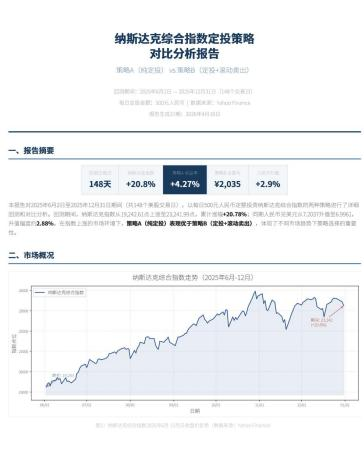
\includegraphics[keepaspectratio,alt={image}]{images/01c28ec58090af663b203f99f261ff27cc2ec6828deaa1e0d55b92e6c599090e.jpg}}

\pandocbounded{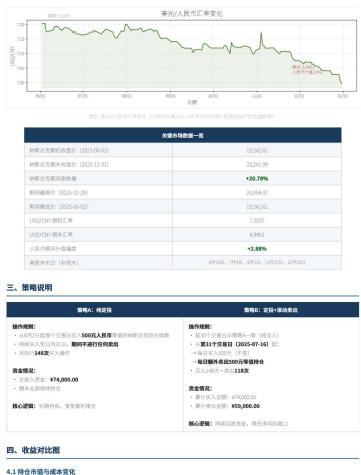
\includegraphics[keepaspectratio,alt={image}]{images/501eb1162d558553286743b3a85c1b256d4192fb40492f42476064109e3d2f71.jpg}}

\pandocbounded{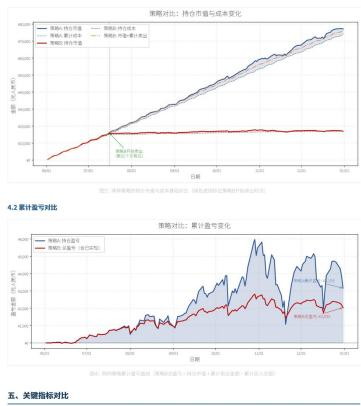
\includegraphics[keepaspectratio,alt={image}]{images/f4e212f9ff214bdb187e35a2c3f3ccddd6eb68dbc5c4103509929e1fb6ab2f89.jpg}}

Figure 14 \textbar{} Example output of a task that requires comparing
two regular investment strategiesfor the NASDAQ.

\pandocbounded{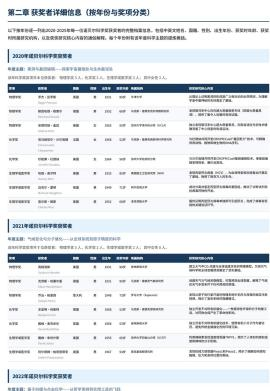
\includegraphics[keepaspectratio,alt={image}]{images/4d5f4a6858d49b05e3c32f64bb6d81eb13c987ae18a9d2ce47ca18dd28dda5e2.jpg}}

\pandocbounded{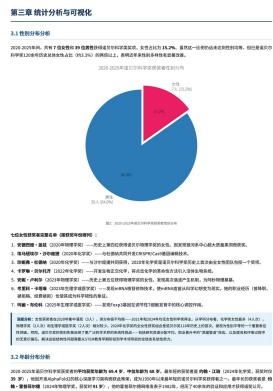
\includegraphics[keepaspectratio,alt={image}]{images/44fc7a2db9816a95d82e5711eb4b3b59bb92adc58af37c8a74e525caae28896b.jpg}}

\pandocbounded{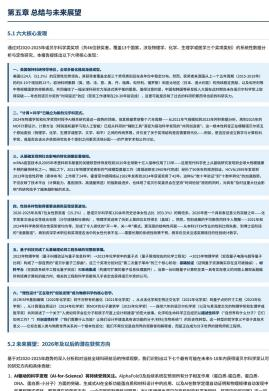
\includegraphics[keepaspectratio,alt={image}]{images/8d32b0afc157e6686e523a2614959155e9f9cfc56b17602f3be8601f58b9a8ee.jpg}}

\pandocbounded{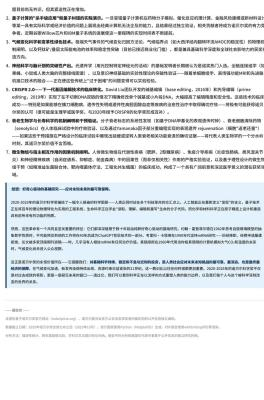
\includegraphics[keepaspectratio,alt={image}]{images/344a4843f90bf72943d28c00d314813c30d42990f744cf2f13ee7b90ec96bef5.jpg}}

Figure 15 \textbar{} Example output of a task which requires researching
2020-2025 Nobel Science Prizesand generating an analytical PDF report.

Table 12 \textbar{} Comparative Analysis of DeepSeek-V4-Pro and
Gemini-3.1-Pro in Chinese FunctionalWriting.

{\def\LTcaptype{none} % do not increment counter
\begin{longtable}[]{@{}lllllllll@{}}
\toprule\noalign{}
\endhead
\bottomrule\noalign{}
\endlastfoot
\multirow{2}{*}{Category} & \multirow{2}{*}{Subcategory} &
\multirow{2}{*}{\#} & \multicolumn{6}{l@{}}{%
Internal Evaluation (内部综合评估)} \\
& & & DS win & Gem win & Tie & DS\% & Gem\% & Tie\% \\
\multirow{10}{*}{Business Writing (办公文本)} & Report (报告) & 527 &
350 & 162 & 15 & 66.41 & 30.74 & 2.85 \\
& Proposal (方案策划) & 291 & 181 & 103 & 7 & 62.20 & 35.40 & 2.41 \\
& Education (教育培训) & 159 & 100 & 56 & 3 & 62.89 & 35.22 & 1.89 \\
& Email \& Letter (邮件书信) & 146 & 107 & 37 & 2 & 73.29 & 25.34 &
1.37 \\
& Notice (通知公告) & 72 & 43 & 24 & 5 & 59.72 & 33.33 & 6.94 \\
& Professional (专业文本) & 63 & 34 & 27 & 2 & 53.97 & 42.86 & 3.17 \\
& Recruitment (招聘求职) & 42 & 27 & 15 & 0 & 64.29 & 35.71 & 0.00 \\
& Technical (技术文本) & 29 & 22 & 7 & 0 & 75.86 & 24.14 & 0.00 \\
& Review (介绍评价) & 20 & 15 & 5 & 0 & 75.00 & 25.00 & 0.00 \\
& Subtotal (小计) & 1349 & 879 & 436 & 34 & 65.16 & 32.32 & 2.52 \\
\multirow{9}{*}{Media Writing (媒体文本)} & Social Media (社交媒体文案)
& 267 & 156 & 101 & 10 & 58.43 & 37.83 & 3.75 \\
& Ad Copy (广告商品文案) & 214 & 109 & 98 & 7 & 50.93 & 45.79 & 3.27 \\
& Long-form Content (内容平台长文) & 99 & 71 & 25 & 3 & 71.72 & 25.25 &
3.03 \\
& News Report (新闻报道) & 51 & 27 & 22 & 2 & 52.94 & 43.14 & 3.92 \\
& Advertorial (营销软文) & 17 & 12 & 4 & 1 & 70.59 & 23.53 & 5.88 \\
& Headline (标题) & 11 & 7 & 4 & 0 & 63.64 & 36.36 & 0.00 \\
& Narration Script (口播文案) & 4 & 2 & 1 & 1 & 50.00 & 25.00 & 25.00 \\
& Comment (评论) & 3 & 2 & 1 & 0 & 66.67 & 33.33 & 0.00 \\
& Subtotal (小计) & 666 & 386 & 256 & 24 & 57.96 & 38.44 & 3.60 \\
\multirow{6}{*}{Everyday Writing (生活文本)} & Congratulatory (祝贺文本)
& 101 & 54 & 41 & 6 & 53.47 & 40.59 & 5.94 \\
& Communication (沟通回复) & 100 & 71 & 26 & 3 & 71.00 & 26.00 & 3.00 \\
& Reflection (心得感想) & 90 & 68 & 17 & 5 & 75.56 & 18.89 & 5.56 \\
& Review (介绍评价) & 55 & 44 & 9 & 2 & 80.00 & 16.36 & 3.64 \\
& Comment (评论) & 44 & 34 & 8 & 2 & 77.27 & 18.18 & 4.55 \\
& Subtotal (小计) & 390 & 271 & 101 & 18 & 69.49 & 25.90 & 4.62 \\
\multirow{6}{*}{Oral Writing (口头文本)} & Speech (发言稿) & 226 & 135 &
85 & 6 & 59.73 & 37.61 & 2.65 \\
& Narration Script (口播文案) & 51 & 25 & 23 & 3 & 49.02 & 45.10 &
5.88 \\
& Sales Script (话术) & 31 & 22 & 6 & 3 & 70.97 & 19.35 & 9.68 \\
& Dialogue (对话文本) & 10 & 4 & 6 & 0 & 40.00 & 60.00 & 0.00 \\
& Congratulatory (祝贺文本) & 1 & 1 & 0 & 0 & 100.00 & 0.00 & 0.00 \\
& Subtotal (小计) & 319 & 187 & 120 & 12 & 58.62 & 37.62 & 3.76 \\
\multirow{6}{*}{Official Document (公文文本)} & Administrative Doc
(事务文书) & 117 & 60 & 53 & 4 & 51.28 & 45.30 & 3.42 \\
& Personal Doc (个人文书) & 73 & 45 & 27 & 1 & 61.64 & 36.99 & 1.37 \\
& Government Doc (行政公文) & 34 & 19 & 14 & 1 & 55.88 & 41.18 & 2.94 \\
& Speech (发言稿) & 3 & 1 & 2 & 0 & 33.33 & 66.67 & 0.00 \\
& Essay Writing (申论写作) & 3 & 1 & 1 & 1 & 33.33 & 33.33 & 33.33 \\
& Subtotal (小计) & 230 & 126 & 97 & 7 & 54.78 & 42.17 & 3.04 \\
\multirow{5}{*}{Academic Writing (学术文本)} & Research Paper (学术论文)
& 104 & 67 & 32 & 5 & 64.42 & 30.77 & 4.81 \\
& Coursework (课程作业) & 90 & 53 & 35 & 2 & 58.89 & 38.89 & 2.22 \\
& Academic Support (学术辅助) & 15 & 11 & 3 & 1 & 73.33 & 20.00 &
6.67 \\
& Science Outreach (专业科普) & 7 & 6 & 1 & 0 & 85.71 & 14.29 & 0.00 \\
& Subtotal (小计) & 216 & 137 & 71 & 8 & 63.43 & 32.87 & 3.70 \\
Total (总计) & & 3170 & 1986 & 1081 & 103 & 62.65 & 34.10 & 3.25 \\
\end{longtable}
}

Table 13 \textbar{} Comparative Analysis of DeepSeek-V4-Pro and
Gemini-3.1-Pro in Chinese CreativeWriting.

{\def\LTcaptype{none} % do not increment counter
\begin{longtable}[]{@{}llllllllllllll@{}}
\toprule\noalign{}
\endhead
\bottomrule\noalign{}
\endlastfoot
\multirow{2}{*}{Subcategory (文体)} & \multirow{2}{*}{\#} &
\multicolumn{6}{l}{%
Instruction Following(指令遵循)} & \multicolumn{6}{l@{}}{%
Writing Quality (写作质量)} \\
& & DS & Gem & Tie & DS\% & Gem\% & Tie\% & DS & Gem & Tie & DS\% &
Gem\% & Tie\% \\
Fiction (小说故事) & 836 & 504 & 323 & 5 & 60.58 & 38.82 & 0.60 & 672 &
157 & 3 & 80.77 & 18.87 & 0.36 \\
General Fiction (泛小说故事) & 662 & 368 & 290 & 3 & 55.67 & 43.87 &
0.45 & 467 & 194 & 0 & 70.65 & 29.35 & 0.00 \\
Fan Fiction (同人文) & 410 & 253 & 150 & 3 & 62.32 & 36.95 & 0.74 & 338
& 67 & 1 & 83.25 & 16.50 & 0.25 \\
General Fan Fic. (泛同人文) & 202 & 111 & 90 & 1 & 54.95 & 44.55 & 0.50
& 161 & 40 & 1 & 79.70 & 19.80 & 0.50 \\
Narrative (记叙文) & 171 & 115 & 54 & 2 & 67.25 & 31.58 & 1.17 & 141 &
30 & 0 & 82.46 & 17.54 & 0.00 \\
General Prose (泛散文) & 124 & 83 & 40 & 1 & 66.94 & 32.26 & 0.81 & 88 &
36 & 0 & 70.97 & 29.03 & 0.00 \\
Prose (散文) & 112 & 74 & 38 & 0 & 66.07 & 33.93 & 0.00 & 92 & 20 & 0 &
82.14 & 17.86 & 0.00 \\
Writing Style (文笔) & 112 & 81 & 31 & 0 & 72.32 & 27.68 & 0.00 & 86 &
26 & 0 & 76.79 & 23.21 & 0.00 \\
Classical Poetry (古诗文) & 48 & 24 & 24 & 0 & 50.00 & 50.00 & 0.00 & 39
& 9 & 0 & 81.25 & 18.75 & 0.00 \\
Modern Poetry (现代诗) & 43 & 23 & 20 & 0 & 53.49 & 46.51 & 0.00 & 32 &
11 & 0 & 74.42 & 25.58 & 0.00 \\
Lyrics (歌词) & 30 & 8 & 22 & 0 & 26.67 & 73.33 & 0.00 & 16 & 14 & 0 &
53.33 & 46.67 & 0.00 \\
Literary Appreciation (赏析) & 27 & 20 & 7 & 0 & 74.07 & 25.93 & 0.00 &
18 & 9 & 0 & 66.67 & 33.33 & 0.00 \\
General Argument. (泛议论文) & 24 & 15 & 9 & 0 & 62.50 & 37.50 & 0.00 &
17 & 7 & 0 & 70.83 & 29.17 & 0.00 \\
General Narrative (泛记叙文) & 23 & 11 & 12 & 0 & 47.83 & 52.17 & 0.00 &
15 & 8 & 0 & 65.22 & 34.78 & 0.00 \\
General Classical (泛古文诗歌) & 9 & 5 & 4 & 0 & 55.56 & 44.44 & 0.00 &
5 & 4 & 0 & 55.56 & 44.44 & 0.00 \\
Creative Writing (创意写作) & 6 & 2 & 4 & 0 & 33.33 & 66.67 & 0.00 & 4 &
2 & 0 & 66.67 & 33.33 & 0.00 \\
Argumentative (议论文) & 5 & 5 & 0 & 0 & 100.00 & 0.00 & 0.00 & 5 & 0 &
0 & 100.00 & 0.00 & 0.00 \\
General Mod. Poetry (泛现代诗) & 2 & 1 & 1 & 0 & 50.00 & 50.00 & 0.00 &
2 & 0 & 0 & 100.00 & 0.00 & 0.00 \\
Total (总计) & 2837 & 1703 & 1119 & 15 & 60.03 & 39.44 & 0.53 & 2198 &
634 & 5 & 77.48 & 22.35 & 0.18 \\
\end{longtable}
}

Table 14 \textbar{} DeepSeek-V4-Pro vs.~Claude-Opus-4.5 on Complex
Instruction Following and Multi-Turn Writing.

{\def\LTcaptype{none} % do not increment counter
\begin{longtable}[]{@{}llllllll@{}}
\toprule\noalign{}
\endhead
\bottomrule\noalign{}
\endlastfoot
\multirow{2}{*}{Category} & \multirow{2}{*}{\#} &
\multicolumn{6}{l@{}}{%
Internal Evaluation (内部综合评估)} \\
& & DS & Opus & Tie & DS\% & Opus\% & Tie\% \\
Complex Inst. Following (复杂指令跟随) & 49 & 23 & 26 & 0 & 46.9\% &
53.1\% & 0.0\% \\
Multi-Turn Writing (多轮写作) & 147 & 67 & 76 & 4 & 45.6\% & 51.7\% &
2.7\% \\
Total (总计) & 196 & 90 & 102 & 4 & 45.9\% & 52.0\% & 2.0\% \\
\end{longtable}
}

\end{document}
